\documentclass[a4paper,12pt]{report}

% Encodage et langues
\usepackage{fontspec}
\setmainfont{Latin Modern Roman}
\usepackage[french]{babel}
\usepackage{listings}
\lstset{
  breaklines=true,
  breakatwhitespace=false,
  basicstyle=\ttfamily\small,
  columns=fullflexible,
}

% Mise en page
\usepackage{geometry}
\geometry{
  a4paper,
  top=2.5cm,
  bottom=2.5cm,
  left=2.5cm,
  right=2.5cm
}
\usepackage{float} 
\usepackage{xcolor}


\usepackage{titlesec}
\definecolor{oxfordblue}{RGB}{0,33,71}
\definecolor{subsectionmaroon}{RGB}{128,0,0}
\titleformat{\section}
  {\color{oxfordblue}\normalfont\Large\bfseries}{\thesection}{1em}{}
\titleformat{\subsection}
  {\color{subsectionmaroon}\normalfont\large\bfseries}{\thesubsection}{1em}{}

%% Plain black formatting for titles
%\titleformat{\section}
% {\normalfont\Large\bfseries}{\thesection}{1em}{}
%\titleformat{\subsection}
 % {\normalfont\large\bfseries}{\thesubsection}{1em}{}


% Set all links to blue
\usepackage[colorlinks=true, 
            linkcolor=black,
            citecolor=blue,
            urlcolor=blue]{hyperref}
\newcommand{\defensedate}{23 juin 2025}

\usepackage{makecell}
\usepackage{etoolbox}
\usepackage{changepage}

% Graphiques et figures
\usepackage{graphicx}
\usepackage{svg}
\usepackage{placeins}
\graphicspath{{images/}{images_pfe/}}

% Tableaux
\usepackage{booktabs}
\usepackage{array}
\usepackage{tabularx}
\usepackage{longtable}
\usepackage{multirow}
\usepackage[table,xcdraw]{xcolor}
\usepackage[footnote]{acronym}

% Listes et énumérations
\usepackage{enumitem}

% Titres - REMOVED COLOR DEFINITIONS


% Bibliographie
\usepackage[%
  backend=biber,
  style=numeric, 
  sorting=nyt,
  language=french,
  autolang=other,
  url=true,
  doi=false,
  isbn=false,
  maxcitenames=1
]{biblatex}
\addbibresource{references.bib}

\usepackage{xurl}
\setcounter{biburllcpenalty}{7000}
\setcounter{biburlucpenalty}{8000}

% En-têtes et pieds de page
\usepackage{fancyhdr}
\pagestyle{fancy}
\fancyhf{}
\lhead{\bfseries\nouppercase{\leftmark}}
\rfoot{\bfseries\thepage}
\renewcommand{\headrulewidth}{1pt}

% Espace inter-paragraphe et interligne
\usepackage{parskip}
\renewcommand{\baselinestretch}{1.05}

% Théorèmes, définitions, etc.
\usepackage{amsthm,amssymb,amsmath}
\newtheorem{definition}{Définition}[chapter]
\newtheorem{theoreme}{Théorème}[chapter]
\newtheorem{remarque}{Remarque}[chapter]
\newtheorem{propriete}{Propriété}[chapter]
\newtheorem{exemple}{Exemple}[chapter]

% Mini-tocs
\usepackage{minitoc}
\setcounter{minitocdepth}{1}
\mtcsettitle{minitoc}{Contenu}

% Required for title page
\usepackage{setspace}
\usepackage{ifthen}
\usepackage{datetime}

% Document title and type
\newcommand{\doctitle}{Développement d'une nouvelle distribution Linux dédiée aux scientifiques}
\newcommand{\doctype}{MÉMOIRE DE FIN D’ETUDES} 

% Informations sur l'université
\newcommand{\department}{DÉPARTEMENT D’INFORMATIQUE ET
DES COMMUNICATIONS}
\newcommand{\degree}{DIPLÔME DE LICENCE EN}
\newcommand{\major}{SCIENCE DE L’INFORMATIQUE}
\newcommand{\defenseDate}{Année Universitaire : 2024-2025}

% Thesis author
\newcommand{\authorName}{NACEF KADDECHI}

% Committee members
\newcommand{\president}{M. Mohamed Tahar Bhiri}
\newcommand{\reviewer}{M. Mohamed Mhiri}
\newcommand{\supervisor}{M. Hedi Tmar}
\newcommand{\cosupervisor}{M. Fares Ayadi}

% PDF Metadata
\newcommand{\keywords}{Linux, distribution, scientifique, open source}
\newcommand{\university}{University of Sfax}
\newcommand{\school}{Faculty of Sciences of Sfax}

\begin{document}

\dominitoc
% ENGLISH TITLE PAGE

\begin{titlepage}
\headheight = 0pt

{%
\fontsize{9pt}{9pt}\selectfont%
\renewcommand\arraystretch{1.8} % Reduced spacing

% Fixed ministry name and department formatting
\begin{longtable}{p{0.35\textwidth} c p{0.35\textwidth}}
\centering RÉPUBLIQUE TUNISIENNE\\
MINISTÈRE DE L'ENSEIGNEMENT\\ SUPÉRIEUR ET DE LA\\ RECHERCHE SCIENTIFIQUE%
& \multirow{3}{*}{\centering 
\includegraphics[width=0.2\textwidth]{images_pfe/logo_fss.png}} 
& \centering \department\\ 
\tabularnewline
\centering ***********\\
\centering UNIVERSITÉ DE SFAX\\
FACULTÉ DES SCIENCES DE SFAX%
& &%
\centering ***********\\
%\centering \textbf{\doctype}\\
\degree~\major%
\tabularnewline%
\end{longtable}
}

\begin{center}
    \begin{spacing}{0.05}
        \makebox[\textwidth]{\rule{520pt}{1.25pt}}\\
        \makebox[\textwidth]{\rule{520pt}{0.75pt}}\\
    \end{spacing}
\end{center}

\vspace*{40pt} % Reduced space

\begin{center}

{
\fontsize{33pt}{33pt}\selectfont%
\textsc{\textbf{\doctype}}\\%
}

\vspace*{12pt}
\textit{présenté à}\\%

\vspace*{3pt}
La Faculté des Sciences de Sfax\\% Fixed capitalization
\department\\%

\vspace*{12pt}
\textit{en vue de l'obtention du}\\%

\vspace*{3pt}
\textsc{\degree~\major}\\%

\vspace*{12pt}
\textit{par}\\%

\vspace*{3pt}
\begin{Large} % Changed to Large
\textbf{\authorName}\\%
\end{Large}

\vspace*{20pt} % Reduced space
{
\begin{spacing}{0.05}
    \rule{300pt}{2pt}\\
    \rule{300pt}{0.75pt}\\
\end{spacing}
\vspace{15pt}
\begin{spacing}{0.9}
    \fontsize{24pt}{24pt}\selectfont% Smaller font
    \textsc{\textbf{\doctitle}}\\%
\end{spacing}
\vspace{5pt}
\begin{spacing}{0.05}
    \rule{300pt}{0.75pt}\\
    \rule{300pt}{2pt}\\
\end{spacing}
}

\vfill
\vspace*{10pt}
\begin{adjustwidth}{-1cm}{0pt} % Shift left by 1cm
\centering
\textbf{soutenu le 23 juin 2025, devant le jury composé de :\\}
\bigbreak
\begin{longtable}{@{}m{0.6\textwidth} m{0.6\textwidth}@{}}
 \president & Président \\
\reviewer & Examinateur \\
\supervisor & Encadrant Académique \\
\cosupervisor & Encadrant Industriel 
\end{longtable}
\end{adjustwidth}
\par

%\begin{longtable}{@{}p{0.6\textwidth} p{0.4\textwidth}@{}}
%\president & Président \\
%\reviewer & Examinateur\\
%\supervisor & Encadrant Académique \\
%\ifstrempty{\cosupervisor}{}{%
%\cosupervisor & Encadrant Industriel 
%\end{longtable}
    
%\end{center}
\vfill
\noindent
\makebox[0.5\textwidth][l]{Année Universitaire : 2025-2026}%
\makebox[0.5\textwidth][r]{Code: LSI - 999999}
\end{titlepage}
\pagenumbering{Roman}
\thispagestyle{empty}
\vspace*{2cm}
\begin{center}
    \huge{\textbf{\textit{Clarification}}}
\end{center}
\vspace{2cm}
\begin{center}
\large{

Certaines informations présentes dans ce mémoire s'appuient sur des ressources externes.\\

Tout au long de ce travail,  le lecteur trouvera des explications techniques détaillées. Celles-ci n'ont pas pour but d'enseigner, mais plutôt d'exprimer mon point de vue personnel  et ce que j'ai véritablement compris de ces concepts.\\
\bigbreak

 Je ne \textbf{prétends} nullement être un expert,Si vous cherchez un exemple d'expertise exceptionnelle dans ce domaine, on peut citer \textbf{Terry A. Davis} \cite{terry_davis}. Celui-ci a créé un système d’exploitation complet nommé \textbf{TempleOS} (incluant son propre langage HolyC, son compilateur, noyau, débogueur, interface graphique, bootloader, shell, etc.).\\
\bigbreak
\bigbreak
\textbf{Ce mémoire et moi-même sommes loin d'atteindre ce niveau,}\\ 
Merci pour votre compréhension.
}
\end{center}
\clearpage
\chapter*{Remerciements}

%\section*{Remerciements}

Avant toute chose, je tiens à exprimer ma profonde gratitude à mon encadrant, \textbf{M. Hedi Tmar}, pour son accompagnement constant, sa disponibilité, sa patience, ainsi que la qualité de ses conseils tout au long de ce travail.

\bigbreak

Je remercie également avec une sincère reconnaissance \textbf{M. Fares Ayadi}, dont le soutien m’a permis d’intégrer l’équipe de Kusa pour effectuer ce stage de fin d’études. Son aide a joué un rôle déterminant dans la concrétisation de ce projet.

\bigbreak

J’adresse enfin mes remerciements aux membres du jury, pour l’honneur qu’ils me font en acceptant d’évaluer ce travail. 

\bigbreak
Je tiens à adresser mes plus sincères remerciements à l’équipe de \textbf{Linux From Scratch (LFS)}~\cite{lfs} pour leur travail remarquable et leur engagement envers la communauté du logiciel libre.\\
Leur documentation (le \textbf{LFS Book}~\cite{lfs_book}) a constitué une véritable pierre angulaire de mon projet, en particulier les premières étapes de compilation croisée et de construction de la chaîne d’outils (voir notre chapitre  \ref{chap:corebuild}) .
\bigbreak
Je souhaite également remercier \textbf{Greg Kroah-Hartman} pour son excellent livre \textit{Linux Kernel in a Nutshell}, que nous avons utilisé dans le chapitre \ref{sec:kernel-boot}, en particulier les chapitres 1 à 6 de son livre. Pour plus de détails , voir la référence~\cite{linux_nutshell}.
\bigbreak
Enfin, je tiens à remercier l’équipe de \textbf{Beyond Linux From Scratch (BLFS)} \cite{blfs} pour nous avoir fourni la base des \textit{bootscripts} (System V), que nous avons enrichie avec nos simple  scripts personnalisés. Leur documentation nous a également servi de référence pour de nombreux paquets que nous avons compilés depuis les sources, en complément d’autres sources telles que les sites officiels, les dépôts GitHub, etc.













\clearpage


\tableofcontents
\clearpage
\listoffigures
\clearpage
\listoftables
\clearpage

% Content of the report
\cleardoublepage
\pagenumbering{arabic}
\chapter*{Liste des sigles et acronymes}
\begin{acronym}[VirtualBox] % Use longest term for spacing

\acro{POSIX}{\emph{Portable Operating System Interface}}
\medskip
\acro{FHS}{\emph{Filesystem Hierarchy Standard}}
\medskip
\acro{LSB}{\emph{Linux Standard Base}}
\medskip


\acro{LFS}{\emph{Linux From Scratch}}
\medskip
\acro{BLFS}{\emph{Beyond Linux From Scratch}}
\medskip
\acro{GNU}{\emph{GNU's Not Unix}}
\medskip
\acro{DNF}{\emph{Dandified Yum (Package Manager)}}
\medskip
\acro{OS}{\emph{Operating System}}
\medskip

\acro{JSON}{\emph{JavaScript Object Notation}}
\medskip
\acro{KDE}{\emph{K Desktop Environment}}
\medskip
\acro{LLVM}{\emph{Low Level Virtual Machine}}
\medskip
\acro{FASM}{\emph{Flat Assembler}}
\medskip
\acro{IR}{\emph{Intermediate Representation}}
\medskip
\acro{DFS}{\emph{Depth-First Search}}
\medskip
\acro{ARM}{\emph{Advanced RISC Machines}}
\medskip

\acro{RAID}{\emph{Redundant Array of Independent Disks}}
\medskip
\acro{LVM}{\emph{Logical Volume Manager}}
\medskip

\acro{KO}{\emph{Kernel Object}}
\medskip
\acro{GRUB}{\emph{GRand Unified Bootloader}}
\medskip
\acro{BIOS}{\emph{Basic Input/Output System}}
\medskip
\acro{UEFI}{\emph{Unified Extensible Firmware Interface}}
\medskip
\acro{Xorg}{\emph{X.Org Server (X Window System)}}
\medskip

\acro{Qt}{\emph{Qt Toolkit (Cross-platform GUI framework)}}
\medskip
\acro{QML}{\emph{Qt Modeling Language}}
\medskip
\acro{SDDM}{\emph{Simple Desktop Display Manager}}
\medskip
\acro{YAML}{\emph{YAML Ain’t Markup Language}}
\medskip
\acro{GPL}{\emph{General Public License}}
\medskip
\acro{CLI}{\emph{Command Line Interface}}
\medskip
\acro{Bash}{\emph{Bourne Again Shell}}
\medskip

\acro{KUR}{\emph{Kraken User Repository}} 
\medskip
\acro{KPM}{\emph{Kraken Package Manager}}
\medskip

\acro{ISO}{\emph{ ISO image format}}
\medskip
\acro{POST}{\emph{Power-On Self-Test}}
\medskip
\acro{VDI}{\emph{Virtual Disk Image }}
\medskip
\acro{RAW}{\emph{Raw Disk Image}}
\medskip

\end{acronym}


\chapter*{Introduction générale} 
\adjustmtc

\addcontentsline{toc}{chapter}{Introduction générale}
\markboth{Introduction générale}{Introduction générale}
\label{chap:introduction}



%\section*{Contexte}
Une grande bataille oppose sans relâche le noyau Windows et le noyau Linux depuis plus de 30 ans.  
Ces deux architectures pilotent le matériel physique des smartphones, ordinateurs, serveurs, jusqu’aux robots d’exploration spatiale.\\

Leur divergence fondamentale est inscrite dans leur ADN :  
\begin{itemize}  
  \item \textbf{Noyau Windows} (hybride) : Privilégie un \textbf{contrôle centralisé} et une architecture homogène  
  \item \textbf{Noyau Linux} (monolithique) : Mise sur la \textbf{modularité} et l’adaptabilité.\\
\end{itemize}  

Le futur vainqueur de cette bataille sera désigné par les scientifiques dont les travaux reposent fondamentalement sur la fiabilité et la flexibilité du système d’exploitation.\\  
En d'autres termes, le système qui saura le mieux \textbf{orchestrer cette intelligence humaine}, en offrant un environnement ultime capable non seulement d’englober tous les domaines scientifiques, mais aussi d’assurer une prise en charge approfondie pour chaque domaine, tout en permettant une transposition instantanée entre eux, sera celui qui marquera l’avenir de la recherche scientifique.\\ \\


\medskip

%\subsection*{Motivation}
 La  flexibilité architecturale  \textbf{modulaire} qui fait du noyau Linux  offre le terreau idéal pour lance ce projet  .  

\textbf{Pourquoi ? \\}  
Le chargement dynamique de modules permet une \textbf{transposition instantanée} du même système d’exploitation vers des environnements spécialisés pour des disciplines variées.  

\medskip
Imaginez :  
\begin{itemize}  
  \item le matin, un laboratoire de physique quantique ;  
  \item l’après-midi, une station de développement web, mobile, cloud ou DevOps ;  
  \item le soir, une plateforme de simulation mathématique.\\  
\end{itemize}  
\clearpage
%\subsection*{Problématique}
Malgré la puissance de cette modularité, la plupart des distributions didie au  grand publique ne l’exploitent pas pleinement.  

Prenons l’exemple d’un ingénieur en informatique travaillant sur le développement d’un logiciel embarqué pour un composant mécanique précis. Il utilise un \textbf{environnement de développement}  (IDE, compilateurs, outils de débogage, etc.) sous une distribution Linux didie aux grand publique, comme Ubuntu ou Fedora \\
Cependant, pour tester le comportement de sa solution, il doit visualiser physiquement le processus dans un 
 \textbf{laboratoire de mécanique}, nécessitant des outils de simulation 3D ou de contrôle en temps réel.
 
Pour valider les performances ou modéliser des aspects complexes, il se tourne vers un  \textbf{laboratoire mathématique}, où des outils de calcul symbolique ou de simulation numérique sont nécessaire

Ces \textbf{allers-retours} entre environnements spécialisés soulignent l’absence d’un système capable de s’adapter \textbf{immédiatement} aux besoins de chaque discipline.\\
\bigbreak
%\subsection*{Objectifs}
Notre projet vise à exploiter la modularité du noyau Linux pour développer \textbf{l’environnement ultime} destiné aux postes de travail scientifiques et académiques, avec :  
\begin{itemize}  
  \item une adaptation immédiate à toute discipline (mathématiques, physique, biologie, informatique, etc.) ;  
  \item une transformation automatique en stations de travail préconfigurées pour chaque spécialité ;  
  \item une philosophie centrée sur les besoins de recherche et les exigences professionnelles des utilisateurs.  
\end{itemize}







\clearpage




\section*{Organisation du mémoire}

Ce mémoire est structuré en trois grandes parties, réparties sur dix chapitres.

\medskip

\begin{description}
  \item[\textbf{Première partie : Contexte, problématique et méthodologie(Chapitres 1)}]  
 Cette première partie présente le cadre général du projet, la société, le contexte du stage ainsi que la problématique identifiée. Une analyse de l’existant est également réalisée, suivie par la présentation de la solution proposée et de la méthodologie adoptée
\bigbreak
  \item[\textbf{Deuxième partie : Architecture et aspects théoriques (Chapitres 2 à 5)\\}]  
  Cette partie fournit les fondements techniques et conceptuels du projet, nécessaires à la compréhension des choix de conception effectués.
  \begin{itemize}
    \item \texttt{Chapitre 2 :} Présentation de l’architecture globale, des standards et des normes retenues.
    \item \texttt{Chapitre 3 :} Les aspects et les mécanismes fondamentaux de la compilation.
    \item \texttt{Chapitre 4 :} Étude des concepts et des mécanismes fondamentaux liés aux gestionnaires de paquets.
    \item \texttt{Chapitre 5 :} Analyse de l’architecture et des choix techniques liés au noyau, au bootloader et aux scripts d’amorçage.
  \end{itemize}
  
\bigbreak
  \item[\textbf{Troisième partie : Développement et implémentation (Chapitres 6 à 10)\\}]  
  Cette dernière partie est dédiée à la réalisation pratique, depuis la phase de développement jusqu’à la génération de l’image ISO.
  \begin{itemize}
    \item \texttt{Chapitre 6 :} Création d’un système de base minimal et fonctionnel.
    \item \texttt{Chapitre 7 :} Rendre le système minimal bootable via la configuration du noyau et du chargeur d’amorçage.
    \item \texttt{Chapitre 8 :} Ajout de composants avancés pour rendre le système plus complet et convivial.
    \item \texttt{Chapitre 9 :} Développement et intégration de notre  gestionnaire de paquets.
    \item \texttt{Chapitre 10 :} Création de l’image ISO bootable de la distribution.
  \end{itemize}
\end{description}

\medskip





\chapter{Contexte général} 
\minitoc
\clearpage
\label{sec:organisme}











%\subsection{Contexte et motivations}

%Dans un monde où la connaissance progresse à un rythme exponentiel, tous les domaines technologiques
%(d'informatique, de mathématiques, de physique, de biologie ou de recherche académique...) dépendent %fondamentalement d'un système d'exploitation. Qu'un chercheur développe une application, programme un %mécanisme expérimental, implémente un algorithme ou rédige une publication scientifique, le choix de %son système d'exploitation (OS) influencera profondément son travail et son potentiel de découverte.


\section{Introduction}
La création d'un système d'exploitation personnalisé  est une tâche complexe qui exige une maitrise approfondie des éléments logiciels et matériels. Ce projet vise à concevoir une distribution Linux optimisée spécifiquement adaptée aux chercheurs et aux scientifiques, en incorporant un gestionnaire de paquet dédié, Kraken.

Dans ce premier chapitre, nous allons présenter le cadre général du projet, l'entreprise d'accueil KUSA  ou  sest deroule le stage par la suite le cadre de projet , letude de lexistant presentant la situaton actuelle , la solution propse et finalement la methode du travail adoptee



%presentation kusa -------




\section{Présentation de l'entreprise KUSA}
\label{sec:kusa}

Fondée en 2020 à Sfax (Tunisie), KUSA est une société de services numériques spécialisée dans le développement de solutions technologiques innovantes. Avec une équipe d'experts en ingénierie logicielle et infrastructure IT, l'entreprise accompagne ses clients dans leur transformation numérique à travers une offre complète de services.

\begin{figure}[hbt!]
  \centering
  
\includegraphics[width=10cm,height=5cm]{images_pfe/kusa.png}
  \caption{Logo officiel de la société KUSA}
  \label{fig:kusa_logo}
\end{figure}
\FloatBarrier
\clearpage
\subsection{Profil de l'entreprise}
\begin{itemize}
    \item \textbf{Siège social} : Sfax, Tunisie
    \item \textbf{Année de création} : 2020
    \item \textbf{Secteurs d'intervention} : 
    \begin{itemize}
        \item Industrie 4.0 et IoT
        \item Commerce électronique
        \item Médias numériques
        \item Solutions d'entreprise
    \end{itemize}
    \item \textbf{Effectif} : Équipe pluridisciplinaire de 15+ experts
\end{itemize}

\subsection{Domaines d'expertise et Méthodologie }
KUSA se positionne comme un intégrateur technologique full-stack offrant :

\subsubsection*{ Développement Sur Mesure}
\begin{itemize}
    \item Applications Web (portails, intranet/extranet, e-commerce)
    \item Solutions mobiles cross-platform (iOS, Android)
    \item Intégrations IoT (systèmes à capteurs, appareils connectés)
    \item Développement d'API et systèmes back-end
    \item Architecture microservices
\end{itemize}

%\subsubsection*{B : Maintenance Applicative (TMA)}
%\begin{itemize}
 %   \item \textbf{Maintenance corrective} : 
  %  \begin{itemize}
   %     \item Correction de bugs et anomalies
    %    \item Résolution d'incidents critiques
   % \end{itemize}
    
   % \item \textbf{Maintenance adaptive} :
    %\begin{itemize}
     %   \item Adaptation aux nouvelles réglementations
      %  \item Migration vers de nouveaux environnements techniques
    %\end{itemize}
    
   % \item \textbf{Maintenance perfective} :
   % \begin{itemize}
    %    \item Optimisation des performances système
     %   \item Amélioration de l'expérience utilisateur (UX)
       
    %\end{itemize}
%\end{itemize}

%\subsubsection*{C : Recette Applicative (TRA)}
%\begin{itemize}
 %   \item Tests fonctionnels
  %  \item Tests de performance
   % \item Tests de non-régression
   % \item Scénarios de test automatisés/manuels
%\end{itemize}



%\subsubsection*{D : Ingénierie Système et Réseau}
%\begin{itemize}
 %   \item Configuration de serveurs/réseaux
  %  \item Infrastructure cloud et virtualisation
   % \item Analyse de performances
    %\item Solutions de sécurité/sauvegarde
%\end{itemize}

\subsubsection*{Méthodologie B.O.T}
Kusa utilise un Modèle de gestion de projet en trois phases :
\begin{itemize}
    \item \textbf{Build} : Conception et développement de solutions sur mesure
    \item \textbf{Operate} : Gestion et optimisation opérationnelle
    \item \textbf{Transfer} : Transmission des compétences avec documentation complète
\end{itemize}

%\subsection{Portfolio Clients}
%Principales collaborations récentes :
%\begin{figure}[hbt!]
%  \centering
 % \begin{minipage}[b]{0.18\textwidth}
  %  
\includegraphics[width=\textwidth]{images_pfe/toyota.jpg}
   % \caption{Toyota}
  %\end{minipage}\hfill
  %\begin{minipage}[b]{0.18\textwidth}
  %  
\includegraphics[width=\textwidth]{images_pfe/aqua.png}
  %  \caption{Aquaressort}
  %\end{minipage}\hfill
  %\begin{minipage}[b]{0.18\textwidth}
   % 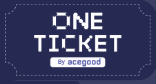
\includegraphics[width=\textwidth]{images_pfe/oneticket.png}
   % \caption*{One Ticket}
  %\end{minipage}\hfill
 % \begin{minipage}[b]{0.18\textwidth}
  %  
\includegraphics[width=\textwidth]{images_pfe/diwan.jpg}
   % \caption{Diwan FM}
  %\end{minipage}\hfill
  %\begin{minipage}[b]{0.18\textwidth}
  %  
\includegraphics[width=\textwidth]{images_pfe/tinusdiscount.png}
   % \caption{TuniDiscount}
  %\end{minipage}\hfill
  %\begin{minipage}[b]{0.18\textwidth}
   % 
\includegraphics[width=\textwidth]{images_pfe/fastosh.png}
    %\caption{Fastosh}
  %\end{minipage}
  %\caption{Clients principaux de KUSA}
  %\label{fig:clients}
%\end{figure}
%\FloatBarrier

\section{Contexte du Stage}
\label{sec:contexte_stage}
Ce stage de fin d'études en licence d'informatique (spécialité génie logiciel) s'est déroulé sur quatre mois au sein de KUSA. L'objectif principal consistait à développer une distribution Linux dédiée à la recherche académique et scientifique

Ce projet s'inscrit dans la stratégie d'innovation de KUSA visant à fournir des solutions open source à la communauté scientifique .
\clearpage
%presentation projet ------------------------------------------------
\section{Présentation du projet}

La plupart des développeurs diront que Linux est un système d’exploitation open source. Ceux qui ont des connaissances plus techniques le qualifieront plutôt de noyau.

Pour moi, cependant, Linux n’est pas seulement un système d’exploitation ou un noyau : c’est la liberté, la liberté de créer un système pour un besoin spécifique


\subsection{Problématique et état de l'existant}

\subsubsection{Le paysage actuel des systèmes d'exploitation}
Trois grands types d'OS dominent aujourd'hui :
\begin{itemize}[leftmargin=*,nosep]
\item Windows (développé par Microsoft)
\item macOS (propriété d'Apple)
\item Distributions Linux (basées sur le noyau open source)
\end{itemize}

Les deux premiers, bien que largement utilisés, souffrent de limitations critiques :
\begin{itemize}[leftmargin=*,nosep]
\item \textbf{Fermeture technologique} : Leur code source propriétaire interdit toute modification profonde
\item \textbf{Dépendance aux géants technologiques} : Leur évolution répond à des logiques commerciales plutôt qu'aux besoins spécifiques de la recherche
\end{itemize}

Seul Linux, par sa philosophie  \textbf{open source} et  \textbf{modularité}, offre une liberté totale de personnalisation.

\begin{figure}[htbp]
    \centering
    
\includegraphics[width=0.85\textwidth]{images_pfe/gnulinux.jpeg}
    \caption{GNU LINUX }
    \label{fig:gnulinux}
\end{figure}


\clearpage







Pourtant, les distributions linux existantes imposent un choix cornélien à nous, membres de la communauté académique et scientifique : opter pour une version grand public ou une version spécialisée.
\begin{itemize}[leftmargin=*,nosep]
    \item \textbf{Distributions destinées au grand public} 

   Habituellement, ces distributions sont conçues pour des tâches quotidiennes élémentaires telles que la navigation web ou la gestion d’activités basiques. C’est le cas, par exemple, de Debian ou Fedora, idéales pour les utilisateurs non experts.
Pour les \textbf{transformer}  en stations de travail adaptées à un domaine spécialisé, une configuration complexe et chronophage s’impose — sans aucune garantie de fonctionnement optimal. Nous devons littéralement les \textbf{forcer} à fonctionner comme nous le voulons, ce qui reste très difficile, surtout sans une expertise approfondie en architecture des systèmes d’exploitation.

   .\begin{figure}[hbt!]
  \centering
  \begin{minipage}[b]{0.18\textwidth}
    
\includegraphics[width=\textwidth]{images_pfe/debian.jpg}
    \caption{Debian}
  \end{minipage}\hfill
  \begin{minipage}[b]{0.18\textwidth}
    
\includegraphics[width=\textwidth]{images_pfe/ubuntu.png}
    \caption{Ubuntu}
  \end{minipage}\hfill
  \begin{minipage}[b]{0.18\textwidth}
    
\includegraphics[width=\textwidth]{images_pfe/fedora.jpg}
    \caption{Fedora}
  \end{minipage}\hfill
  \begin{minipage}[b]{0.18\textwidth}
    
\includegraphics[width=\textwidth]{images_pfe/redhat.png}
    \caption{Redhat}
  \end{minipage}\hfill
  \begin{minipage}[b]{0.18\textwidth}
    
\includegraphics[width=\textwidth]{images_pfe/archlinux.png}
    \caption{ArchLinux}
  \end{minipage}\hfill
  
  
  \caption{Distributions destinées au grand public}
  \label{fig:distributions destine au grand public}
\end{figure}
\FloatBarrier

    
   

    \item \textbf{Distributions spécialisées}
    
   Ces distributions ciblent une petite catégorie d’utilisateurs, C’est le cas, par exemple de  Kali Linux , Tails OS ou Blackarch. Généralement, elles sont construites \textbf{ à partir} d’une distribution existante destinée au grand public. L’idée sous-jacente est d’extraire de leur distribution mère certains environnements et outils pour un domaine spécifique, \textbf{sans apporter de modifications radicales}. \\ Par conséquent, elles héritent fondamentalement de la majorité des problèmes inhérents aux distributions grand public. 



   .\begin{figure}[!hbt!]
  \centering
  \begin{minipage}[b]{0.18\textwidth}
    
\includegraphics[width=\textwidth]{images_pfe/kalilinux.png}
    \caption{KaliLinux}
  \end{minipage}\hfill
  \begin{minipage}[b]{0.18\textwidth}
    
\includegraphics[width=\textwidth]{images_pfe/alpine.jpg}
    \caption{Alpine linux }
  \end{minipage}\hfill
  \begin{minipage}[b]{0.18\textwidth}
    
\includegraphics[width=\textwidth]{images_pfe/void.png}
    \caption{Void Linux}
  \end{minipage}\hfill
  \begin{minipage}[b]{0.18\textwidth}
    
\includegraphics[width=\textwidth]{images_pfe/tailsosos.png}
    \caption{Tails os}
  \end{minipage}
  
  \caption{Distributions spécialisées}
  \label{fig:distributions spécialisées}
\end{figure}
\FloatBarrier

   

  \subsection{Quel type de distribution dois-je choisir ?} 
  
\textbf{En tant qu'utilisateur académique et scientifique, quel type de distribution dois-je choisir ?}

Cela peut  surprendre, mais la réponse est : aucun des deux.

\begin{itemize}
    \item \textbf{S’il décide de choisir une distribution dédiée au grand public} (ex. : Debian ou une autre généraliste), il rencontrera inévitablement ces problèmes :
    \begin{enumerate}[label=\Alph*)]
        \item Surcharge logicielle inutile pour son travail.
        \item Configuration complexe pour les outils scientifiques $\rightarrow$ Il ne trouve pas tous les outils de domaine préconstruits et installés. Il devra les ajouter manuellement aux dépôts ou les compiler depuis les sources.
        \item Consommation élevée de ressources $\rightarrow$ Conçue pour le grand public, elle installera par défaut une combinaison d’outils pour tous types d’utilisateurs.
        \item Obligation d’utiliser une interface utilisateur ne correspondant pas à son identité scientifique.
        \item Perte de temps à attendre les mises à jour et nouvelles versions des paquets $\rightarrow$ Les scientifiques ne sont pas la catégorie prioritaire pour les mainteneurs de cette distribution.\\
    \end{enumerate}
    
    \item \textbf{S’il opte pour une distribution spécialisée} (ex. : Kali Linux, tailsos, blackarch) :
    \begin{enumerate}[label=\Alph*)]
        \item Malheureusement, il n’existe pas de distribution spécialisée pour chaque domaine scientifique spécifique.
        \item Impossibilité de s’adapter aux projets multidisciplinaires $\rightarrow$ Exemple : S’il utilise Kali Linux et souhaite exploiter des outils de mathématiques ou de physique, il rencontrera d’énormes difficultés en tant que non-expert en systèmes d’exploitation.
        \item Ces distributions sont conçues pour des niches d’utilisateurs, souvent trop restreintes, ce qui entraîne un manque de mainteneurs motivés $\rightarrow$ Paquets et outils obsolètes ou abandonnés.
    \end{enumerate}
\end{itemize}



\subsection{Analyse des distributions Linux académiques scientifiques}

Il existe déjà plusieurs distributions Linux pour les chercheurs et les scientifiques. La plupart sont \textbf{abandonnées} car elles présentent quelques limitations. Voici ce tableau qui indique les principales distributions scientifiques/académiques existantes et leurs limitations :

\begin{table}[H]
\centering
\begin{tabularx}{\textwidth}{|l|X|l|X|}
\hline
\textbf{Distribution} & \textbf{Public cible} & \textbf{Statut} & \textbf{Problèmes courants} \\
\hline
Scientific Linux & Physique des hautes énergies, analyse de données & Abandonné (2021) & Paquets obsolètes, support matériel limité \\
\hline
Bio-Linux & Génomique, phylogénétique & Abandonné (2016) & Dépendances conflictuelles, dépôts vieillissants \\
\hline
Fedora Scientific & Calcul scientifique général & Actif & Cycle de mise à jour trop rapide, outils limités \\
\hline
Ubuntu Studio & Production multimédia & Actif & Problèmes de compatibilité avec les applications hors multimédia \\
\hline
\end{tabularx}
\caption{Comparaison avec les distributions Linux académiques/scientifiques existantes}
\label{tab:comparaison}
\end{table}




\textbf{Enfin, nous avons cru avoir trouvé une distribution scientifique toujours active et non abandonnée !} \\
Malheureusement, ce n’est pas le cas. Prenons l’exemple de Fedora Scientific, l’une des grandes distributions scientifiques actives :

\begin{itemize}
    \item[A.] Cette distribution est parrainée par une entreprise nommée Red Hat.  une entreprise  qui a récemment choqué la communauté open source en restreignant brusquement l’accès au code source de RHEL (Red Hat Enterprise Linux), ce qui a entraîné une \textbf{perte de confiance}  des utilisateurs. En effet, certains craignent que Fedora Scientific, étant liée à Red Hat, ne soit un jour transformée en produit commercial payant, exigeant un abonnement pour accéder à ses outils
    
    \item[B.] \textbf{Terrain d’essai:} Fedora science est la distribution en amont de RHEL, servant de plateforme de test et d’innovation pour Red Ha.Concrètement, les utilisateurs de Fedora sont des \textbf{rats de laboratoire}  , les nouvelles fonctionnalités, les mises à jour logicielles et les noyaux expérimentaux y sont déployés en premier. Une fois stabilisés et débogués grâce aux retours de la communauté, ces paquets sont intégrés à RHEL
    
    \item[B.] \textbf{ Outils préinstallés problématiques :} Elle inclut une suite étendue d’outils scientifiques préinstallés, entraînant :
        \begin{itemize}
            \item Un gaspillage d’espace disque .
            \item Conflits de dépendances et ralentissements sur machines 
        \end{itemize}
    
  \item[C.] \textbf{Cycle de publication :} Fedora Science publie de nouvelles versions tous les 6 mois : donc il devra attendre six mois pour toute mise à jour du système, noyau et pilotes inclus.

    \item[D.] \textbf{Limitations du gestionnaire de paquets :}  DNF est plus lent et limité en raison de ses dépôts , ce qui ralentit la résolution des dépendances.
    
  \item[E.]  \textbf{Environnements non isolés et dépendances externes :} Dépendance à des logiciels tiers et services externes (non maintenus par l’équipe Fedora). De plus, aucune séparation n’existe entre les environnements de chaque domaine. Il héritera donc de dizaines d’outils inutiles pour un besoin spécifique.
\end{itemize}


\textbf{Les problèmes principaux sont :}
\begin{enumerate}[label=\alph*)]
    \item Complexité de configuration
    \item Problèmes de pilotes et compatibilité
    \item Spécialisation mono-domaine
    \item Limitations de personnalisation de l’interface
    \item Courbe d’apprentissage difficile
    \item Problèmes de dépendances
    \item Risque d’abandon à tout moment
    \item Problèmes de confiance au sein de la communauté open source
\end{enumerate}
\clearpage
\subsection{Solution proposée par notre distribution}

\subsubsection{Le paradoxe à résoudre}
\textbf{Comment concilier deux exigences apparemment contradictoires ?}
\begin{itemize}
\item \textbf{Préserver les fondamentaux }: Assurer toutes les fonctions de base d'un OS moderne
\item \textbf{Offrir une flexibilité radicale }: Permettre à l'OS de se transformer en :
\begin{itemize}
\item Laboratoire de mathématiques
\item Station de développement (mobile, web, desktop, cybersécurité)
\item Environnement de simulation physique
\item Plateforme d'analyse génomique
\item Environnement de physique computationnelle
\item Station de développement IA/ML
\end{itemize}
\end{itemize}
\textbf{Cohabitation sans conflits :} Tous ces environnements spécialisés peuvent fonctionner simultanément sur le même système, sans interférences ni incompatibilités \\ 
\\
\\

 Pour répondre à ces défis, nous développons une distribution Linux adaptée aux besoins des scientifiques et chercheurs, visant à combler les lacunes problématiques des distributions scientifiques existantes


\subsection{Pourquoi choisir Kraken OS ?}

\textbf{Kraken OS} a priorisé la résolution méthodique des lacunes et problématiques critiques recensées dans les distributions existantes, grâce à des mécanismes novateurs et une refonte philosophique profonde de son architecture

\begin{itemize}
    
    
    \item \textbf{Comment résolvons-nous le problème des dépendances ?}\\ Pour éviter la dépendance aux distributions mères dédiées au grand public, nous construisons notre système depuis les sources, assurant un \textbf{contrôle total}. \\
    
    \item \textbf{Comment résolvons-nous le problème de stabilité ?}\\ Nous avons implémenté un nouveau gestionnaire de paquets utilisant un mécanisme hybride, offrant à la fois des mises à jour en rolling release et une base stable. \\
    
    \item \textbf{Comment résolvons-nous le problème des paquets inutiles préinstallés ?}\\ Un mécanisme de sélection modulaire permet de choisir strictement les paquets par domaine scientifique, garantissant une séparation claire.\\
    
    \item \textbf{Comment résolvons-nous le problème des multi-environnements ?}\\ Un système de basculement fluide entre environnements spécialisés (mathématiques, informatique, physique, etc.) a été intégré.
    \\
    \item \textbf{Comment résolvons-nous le problème des limitations de personnalisation ?}\\ Nous fournissons des environnements graphiques complets adaptés à l’identité de chaque domaine. \\
    \textbf{Note :} L’utilisateur dispose également de tous les outils pour personnaliser son environnement selon ses besoins.
    \\
    \item \textbf{Comment résolvons-nous le problème de confiance ?} \\L’intégralité du projet est développée sous une philosophie open source stricte.\\
    
    \item \textbf{Comment résolvons-nous le problème de complexité de configuration ?}\\ Un mécanisme de post-installation automatisé dans le gestionnaire de paquets gère toutes les configurations nécessaires (fichiers de paquets, liens symboliques, entrées de bureau, activation au démarrage, etc.).\\
    \item \textbf{Comment résolvons-nous le problème de d’apprentissage difficile ?}\\Des tutoriels interactifs complets, organisés par domaine scientifique et par outil, sont intégrés au système.\\
\end{itemize}
\clearpage
 \subsection{ Pourquoi Kraken OS redéfinit les standards des systèmes scientifiques ?} \\ \\
Cette distribution sera capable de :
\begin{enumerate}[label=\alph*)]
\item Assurer le bon fonctionnement des fondamentaux d’un système d’exploitation moderne :
\begin{itemize}
\item Gestion mémoire 
\item Contrôle des périphériques et pilotes
\item Orchestration des processus et threads
\item Système de fichiers évolutif
\end{itemize}

\item Fournir une interface personnalisable et conviviale  :
\begin{itemize}
\item Gestionnaires de fenêtres personnalisés (GNOME/KDE)
\item Profils visuels par discipline (MATH ,PHYSIQUE , INFORMATIQUE ...)
\end{itemize}

\item Fournir tous les outils préconfigurés nécessaires via le gestionnaire de paquets "Kraken" :
\begin{itemize}
\item Catalogue modulaire validé (paquets validés par la communauté scientifique)
\item Gestion des interdépendances multi-domaines
\end{itemize}

\item Environnement sécurisé :
\begin{itemize}
\item Isolation des expérimentations critiques
\item Authentification, Autorisation, Audit
\end{itemize}

\item Faciliter l’installation et la configuration des outils de recherche : 
\begin{itemize}
\item Assistants d'installation contextuels (workflows guidés par domaine)
\item Configuration automatique des environnements
\end{itemize}

\item Flexibilité interdisciplinaire :
\begin{itemize}
\item Bascules rapides entre domaines scientifiques
\item Gestion des conflits de dépendances multi-domaines
\end{itemize}

\item Optimisation des performances scientifiques :
\begin{itemize}
\item Compilation pour calcul intensif
\item Gestion des ressources GPU/CPU
\end{itemize}

\item Compatibilité matérielle :
\begin{itemize}
\item Pilotes pour instruments de laboratoire
\item Support des protocoles scientifiques
\end{itemize}

\item Documentation :
\begin{itemize}
\item Aide intégrée par discipline
\item Tutoriels interactifs par domaine \\ 
 \\ 
 \\
\end{itemize}
\end{enumerate}


\textbf{
Kraken OS est bien plus qu’un simple système d’exploitation : c’est l’environnement ultime pour un poste de travail scientifique ou académique, quelle que soit la discipline concernée. Les besoins en recherche et les exigences professionnelles sont placés au cœur de la philosophie du système.
}







\section{Méthodologie de travail}
Durant notre stage chez KUSA, nous avons adopté la méthodologie Agile, plus précisément le cadre Scrum pour résoudre notre probléme et trouver des solutions pour faciliter n'importe quelle tâche . 
%\subsection{Présentation de la méthode SCRUM}

Scrum signifie mêlée en français, ce cadre méthodologique agile révolutionne la manière dont on gére un projet dont lequel l'équipe se réuni le plus souvent possible afin de vérifier que le projet avance correctement. Il permet de délivrer et de modifier un projet, un produit ou une foctionnalité très rapidement. 

L'équipe Scrum est composée de:
\begin{itemize}
    \item 	Product Owner :

Il porte la vision de produit à créer, et c'est donc souvent un expert de domaine. l travaille en collaboration directe avec l’équipe de développement et a notamment la charge de remplir le Backlogproduit et de déterminer la priorité des user stories à réaliser.

      \item 	Scrum Master :

c'et un membre de la part entiére de l'équipe projet, et il doit maîtriser Scrum car il est charger de garantir que la méthodologie est appliquée correctement.

        \item Équipe de développement :

Elle regroupe les personnes qui seront responsabe de la de la mise en oeuvre des besoins des clients. Cette équipe est habituellement composée de développeurs, testeurs et d'autres membre pertinents .

\end{itemize}

La figure représente à la fois les différents  rôles de Scrum que nous venons de montrer et le déroulement de processus .

\label{sec:hotspot}
La figure \ref{fig:scrum} représente le cycle de vie SCRUM.
\begin{figure}[hbt!]
  \centering
  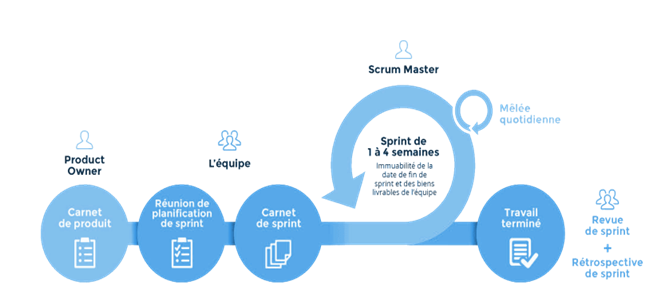
\includegraphics[width=17cm]{images_pfe/scrum.png}
  \caption{Cycle de vie SCRUM.}
  \label{fig:scrum}
\end{figure}
\FloatBarrier

\section{Conclusion}
Ce chapitre présente une étude préliminaire du projet dans lequel  nous avons d'abord exposé le cadre et la problématique et les motivations ayant conduit au développement de cette  distribution Linux.

Dans le prochain chapitre, nous allons examiner la phase d'architecture et les choix techniques qui ont orienté la conception du système et du gestionnaire du paquets Kraken.
 
\medskip



      









  
            

        




  

















% Architecture chapters
\chapter{Architecture Generale et Choix Techniques} \label{chap:archgenerale}
\minitoc
\clearpage


\section{Introduction}

La création d’une distribution Linux personnalisée implique des décisions techniques et conceptuelles rigoureuses afin de garantir la \textbf{compatibilité} du système avec le matériel et les logiciels existants.  \\

Dans ce chapitre, nous allons  présenter : Architecture Générale de notre système, architecture cible  et   à quel ensemble de standards   nous appartenons.

 


\section{Architecture générale de la distribution Linux}
Avant de détailler chaque composant, il est essentiel de décrire le cadre général du système et de préciser les architectures matérielles que nous visons.

\begin{figure}[htbp]
    \centering
    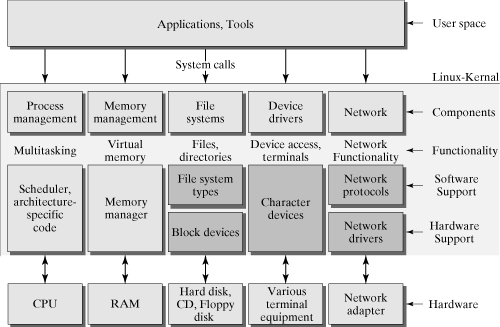
\includegraphics[width=1\textwidth]{images_pfe/linuxarchi.png}
    \caption{Couches de l’architecture d’un système Linux}
    \label{fig:linux-archi}
\end{figure}

Comme le montre la figure, un système se compose de trois couches principales :

\begin{enumerate}
  \item \textbf{Couche matérielle} : regroupe tous les périphériques physiques (RAM, disque dur, processeur, etc.).
  \item \textbf{Noyau} : composant central du système d’exploitation, il interagit directement avec le matériel et fournit des services bas niveau aux couches supérieures. \textcolor{blue}{(Nous en discuterons en détail au chapitre \ref{subsec:noyau-modules}}.)
  \item \textbf{Espace utilisateur} :  
    \begin{itemize}
      \item \textbf{Shell} : interface avec le noyau, masquant sa complexité et transmettant les commandes de l’utilisateur aux \textbf{appels système}.
      \item \textbf{Utilitaires} : programmes fournissant la majeure partie des fonctionnalités offertes à l’utilisateur.
    \end{itemize}
\end{enumerate}

Pour bien cadrer notre distribution, deux questions doivent guider nos choix :

\begin{enumerate}[label=\arabic*)]
  \item Quelles architectures matérielles cibles souhaitons-nous supporter ?
 % \item Quel noyau  allons-nous utiliser ?
  \item Quels standards  devons-nous utiliser pour assurer la portabilité et la compatibilité ?
\end{enumerate}

\section{Architectures physique cibles}
\label{subsec:arch-cibles}

. Le choix des architectures cibles conditionne en effet les outils de compilation, les optimisations et les bibliothèques à intégrer.

\begin{table}[htbp]
  \centering
  \caption{Types d’architectures de processeur (exemple)}
  \label{tab:architectures}
  \begin{tabular}{|l| l| c| l|}
    \toprule
    \textbf{Architecture} & \textbf{Type} & \textbf{Largeur (bits)} & \textbf{Cas d'utilisation} \\
    \midrule
    x86-64   & CISC & 64           & Stations de travail, serveurs \\ \hline
    ARM64    & RISC & 64           & Mobile, embarqué, serveurs    \\ \hline
    MISP    & RISC   &  32 / 64      & Routeurs, systèmes embarqués, usage éducatif \\ \hline
    RISC-V   & RISC & 32/64/128    & Usage académique, matériel sur mesure \\\hline
    POWER    & RISC & 64           & Serveurs d'entreprise, calcul haute performance \\
    \bottomrule
  \end{tabular}
\end{table}

Dans notre distribution , nous avons choisi comme architectures cibles  les processeurs \textbf{AMD et Intel x86\_64 }, en raison de leur compatibilité étendue et de leur support matériel mature. 


%\section{Pourquoi choisir le noyau Linux plutôt que le noyau Windows ?}

%\subsection*{1. Architecture}
%Le noyau Windows est souvent décrit comme un noyau hybride, combinant des éléments de micro- et de noyau monolithique : un microcœur gère les fonctions de %base, tandis que des composants comme les pilotes et systèmes de fichiers s’exécutent en mode noyau.  
%Le noyau Linux est principalement monolithique : tous les services nécessaires (pilotes, systèmes de fichiers, etc.) sont intégrés dans un bloc unique de %code s’exécutant en mode noyau.

%La distinction entre mode utilisateur et mode noyau existe dans les deux cas, mais Windows sépare strictement applications et opérations noyau, alors que %Linux expose davantage de fonctionnalités et de flexibilité dans le noyau lui-même.

%\subsection*{2. Philosophie de conception}
%\begin{itemize}
 % \item \textbf{Windows} : noyau propriétaire développé par Microsoft ; personnalisation et transparence limitées.  
 % \item \textbf{Linux} : noyau open source, modifiable et redistribuable librement.  
  %  Il supporte les modules noyau dynamiques, pouvant être chargés ou déchargés à chaud, offrant une grande flexibilité et facilitant mises à jour et %personnalisations.
%\end{itemize}

%\subsection*{3. Gestion des processus}
%Les deux noyaux assurent une isolation forte des processus, mais Linux offre un contrôle plus granulaire de l’ordonnancement et de l’allocation des %ressources (cgroups, nice, etc.).

%\subsection*{4. Gestion de la mémoire virtuelle}
%\begin{itemize}
%  \item \textbf{Windows} : mémoire virtuelle complexe avec fichier d’échange (pagefile) et compression en mémoire.  
%  \item \textbf{Linux} : pagination à la demande et mécanismes de cache agressifs, souvent plus performants. De nombreux outils (Valgrind, perf) facilitent le suivi et la détection de fuites de mémoire.
%\end{itemize}

%\subsection*{5. Pilotes de périphériques}
%\begin{itemize}
 % \item \textbf{Windows} : modèle de pilote spécifique, large prise en charge matérielle, mais signature Microsoft requise pour la sécurité.  
  %\item \textbf{Linux} : chargement dynamique des pilotes en modules, simplifiant l’ajout de nouveaux matériels sans redémarrage.
%\end{itemize}

%\subsection*{6. Appels système et API}
%\begin{itemize}
 % \item \textbf{Windows} : API riche (WinAPI) étroitement liée au noyau.  
  %\item \textbf{Linux} : ensemble d’appels système standardisés, utilisé par les applications pour invoquer les services du noyau.
%\end{itemize}

%\bigskip
%\noindent
%\textbf{En résumé}, le noyau Linux nous offre :
%\begin{itemize}
 % \item Un contrôle total du code source pour une personnalisation extrême,  
 % \item Une gestion fine de la mémoire et des ressources,  
 % \item Un pilotage précis des appels système,  
 % \item La capacité de charger et décharger immédiatement des pilotes matériels via les modules, sans redémarrage.
%\end{itemize}


\section{Normes de notre distibution}
\label{subsec:standards}

La structure de du systeme  respecte  les standards Linux suivants :

\begin{itemize}
  \item \textbf{POSIX}  
  \item \textbf{FHS } 
  \item \textbf{LSB  }
\end{itemize}


\subsection{POSIX}
\label{sssec:posix}
La norme POSIX (Interface portable pour systèmes d'exploitation) a été conçue pour standardiser un ensemble de fonctionnalités essentielles qu’un système d'exploitation doit fournir. Elle spécifie notamment une interface de programmation, un shell de commande ainsi qu’un ensemble d'outils classiques, dans le but de rendre les logiciels facilement transférables entre différentes plateformes de type Unix. 

\paragraph{Pourquoi POSIX est‑il important ?}
\begin{enumerate}
  \item Assurer la \textbf{portabilité} des logiciels entre systèmes de type UNIX (Linux, macOS, BSD, etc.).
  \item Fournir une API cohérente pour les appels système, la gestion des fichiers et le pilotage des processus.
  \item Aider les développeurs à écrire des applications \textbf{cross‑platform} sans réécrire leur code pour chaque OS.
\end{enumerate}


\textcolor{blue}{Pour plus d’informations sur POSIX, consultez \cite{posix}}

\subsection{Filesystem Hierarchy Standard (FHS) }
\label{sssec:fhs}
Le standard FHS (Filesystem Hierarchy Standard) définit une organisation logique des fichiers et répertoires dans les systèmes de type UNIX. Son objectif est d’assurer une cohérence dans la structure du système, facilitant ainsi la compatibilité des logiciels, des outils d’administration et des scripts. Il permet également de maintenir une documentation structurée et homogène entre différentes distributions Linux 



La structure de \textsc{Kraken OS} suit scrupuleusement ce standard (voir figure\textcolor{blue}{~\ref{fig:fsl}}).

\begin{figure}[H]
  \centering
  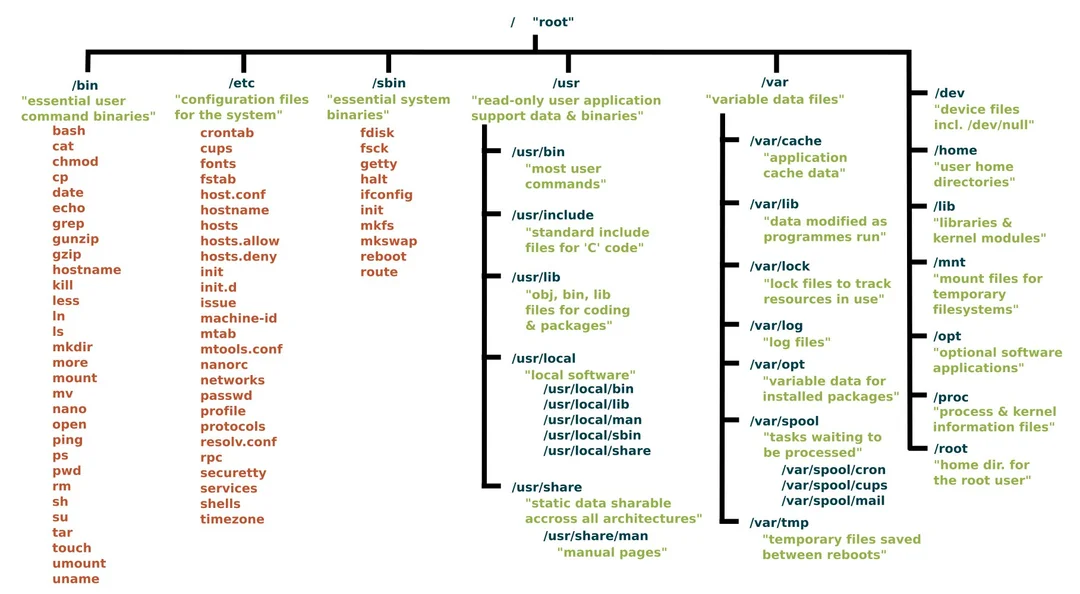
\includegraphics[width=0.85\textwidth]{images_pfe/fslinux.png}
  \caption{Architecture du système de fichiers conforme au standard FHS }
  \label{fig:fsl}
\end{figure}




Les principaux répertoires comprennent :

\begin{itemize}
    \item \textbf{Répertoires essentiels} :
    \begin{itemize}
        \item \texttt{/bin}, \texttt{/sbin} : Liens symboliques vers \texttt{/usr/bin} et \texttt{/usr/sbin} (conformément aux bonnes pratiques de sécurité)
        \item \texttt{/lib}, \texttt{/lib64} : Liens vers \texttt{/usr/lib} et \texttt{/usr/lib64} (centralisation des bibliothèques)
    \end{itemize}
    
    \item \textbf{Répertoires systèmes critiques} :
    \begin{itemize}
        \item \texttt{/etc} : Configuration système globale (fichiers \texttt{.conf}, scripts d'initialisation)
        \item \texttt{/var} : Données volatiles (logs, bases de données, files d'attente)
        \item \texttt{/proc}, \texttt{/sys} : Interfaces virtuelles pour le monitoring du kernel
    \end{itemize}
    
    \item \textbf{Répertoires fonctionnels} :
    \begin{itemize}
        \item \texttt{/sources} : Isolation des sources logicielles et artefacts de compilation
        \item \texttt{/tools} : Chaîne d'outils temporaire (compilateur croisé, utilitaires bootstrap)
       \item \texttt{/opt} : répertoire dédié aux applications autonomes (monolithiques), comme KDE Frameworks ou Qt6, afin d’éviter les conflits de dépendances qui pourraient survenir lors d’une installation dans un repertoire classique come /usr 

    \end{itemize}
    
    \item \textbf{Répertoires opérationnels} :
    \begin{itemize}
        \item \texttt{/dev} : Représentation hiérarchique des périphériques
        \item \texttt{/mnt}, \texttt{/media} : Points de montage temporaires
        \item \texttt{/srv} : Données spécifiques aux services 
        \item \texttt{/tmp} : Fichiers temporaires (nettoyage automatique via \texttt{tmpfs})
    \end{itemize}
\end{itemize}

Cette architecture répond à trois impératifs fondamentaux :
\begin{enumerate}
    \item Séparation stricte entre composants systèmes et données utilisateur
    \item Isolation des processus de compilation via \texttt{/sources} et \texttt{/tools}
    \item Compatibilité avec les mécanismes kernel (montage automatique de \texttt{/proc}, \texttt{/sys})
\end{enumerate}


\textcolor{blue}{Pour plus d’informations sur FHS, consultez \cite{FHS}}

\subsection{Linux Standard Base (LSB) }
\label{sssec:lsb}
La LSB (Linux Standard Base) a pour but de favoriser la compatibilité des logiciels, en particulier propriétaires, avec les systèmes Linux qui respectent ses règles. Elle repose sur un ensemble de quatre modules distincts, chacun couvrant un aspect spécifique du système

\begin{table}[htbp]
  \centering
  \caption{Spécifications de la LSB v5.0}
  \label{tab:lsb-specs}
  \begin{tabular}{|l| p{8cm}|}
    \toprule
    \textbf{Module} & \textbf{Description} \\
    \midrule
   Modules de base    & Interface système de base et utilitaires essentiels (ex:glibc,bash,coreutils)) \\ \hline
    Environnements graphiques  & Composants graphiques et bibliothèques pour environnements de bureau(ex : alsa-lib,gtk)  \\ \hline
    Langages & Bibliothèques de support pour langages et formats (ex: libxml) \\  \hline
    Traitement d'images & Services d’impression et traitement d’images (ex:cups)  \\
    \bottomrule
  \end{tabular}
\end{table}


%Étant donné que \textsc{Kraken OS} est compilé intégralement à partir des sources, nous %vérifions à la compilation que chaque paquet respecte les exigences LSB. Par exemple :

%\begin{itemize}
 % \item \textbf{Core} : \texttt{bash}, \texttt{coreutils}, \texttt{glibc}, \texttt{binutils}, %\texttt{diffutils}, \texttt{grep}, \texttt{gzip}, \texttt{m4}, \dots  
 % \item \textbf{Desktop} : \texttt{alsa-lib}, \texttt{atk}, \texttt{cairo}, \texttt{glib2}, %\texttt{gdk-pixbuf}, \texttt{gtk+}, \texttt{fontconfig}, \dots  
 % \item \textbf{Languages} : \texttt{libxml2}, \texttt{libxslt}, \dots  
 % \item \textbf{Imaging} : \texttt{cups}, \texttt{cups-filters}, \texttt{ghostscript}, %\texttt{sane-backends}, \dots  
%\end{itemize}

\textcolor{blue}{Pour plus d’informations sur LSB, consultez \cite{LSB}}
\section{Conclusion}

\bigskip
\noindent
En respectant rigoureusement ces standards — POSIX, FHS et LSB — Notre system  affirme son appartenance à la grande famille 
nommer UNIX‑like (BSD , macOS, LINUX ... ).\\
Les utilisateurs et développeurs savent ainsi qu’ils peuvent porter et exécuter leurs applications POSIX sur notre systeme  sans adaptation majeure, bénéficier d’une hiérarchie de fichiers prévisible et d’une compatibilité garantie avec les logiciels tiers conformes à la LSB.





\chapter{Compilation depuis la source} 
\minitoc
\label{ssse:compilation-source}

\clearpage


\section{Introduction}
Comme nous l'avons évoqué, notre système sera construit entièrement à partir des sources, afin de garantir une indépendance totale vis‑à‑vis des distributions grand public. Nous devons donc étudier les mécanismes et les problématiques liés à la compilation.


\section{Qu’est‑ce qu’un paquet ?}
\label{sssec:definition-paquet}

Un \emph{paquet} est un ensemble de fichiers (bibliothèques, scripts, documentation) fournissant une fonctionnalité précise dans le système : ce paquet peut être un compilateur (\texttt{gcc}), un utilitaire de liens (\texttt{binutils}), un outil de recherche de fichiers (\texttt{findutils}), un utilitaire de base (\texttt{coreutils}), un backend de compilation (\texttt{LLVM}), etc.

Généralement, ce paquet est compressé sous un format tar.gz ,tar.xz,tar.bz2 ou zip, que l’on peut obtenir depuis le site officiel ou en clonant le dépôt GitLab/GitHub.\\
Il contient le code source  et \textbf{un système de build} décrivant comment compiler le paquet.\\ Parfois, il inclut aussi les sources de tiers nécessaires à la construction : par exemple, si le programme final executable est lié dynamiquement à \texttt{libc}, l’auteur du paquet peut inclure une version locale de \texttt{glibc}  dans ses sources.\\
\bigbreak
\textbf{Question :} Les execuatble  sont-ils liés dynamiquement ? 

Cette question est cruciale dans un système Linux et nous amène naturellement à distinguer les bibliothèques statiques et les bibliothèques partagées.

\begin{figure}[H]
  \centering
  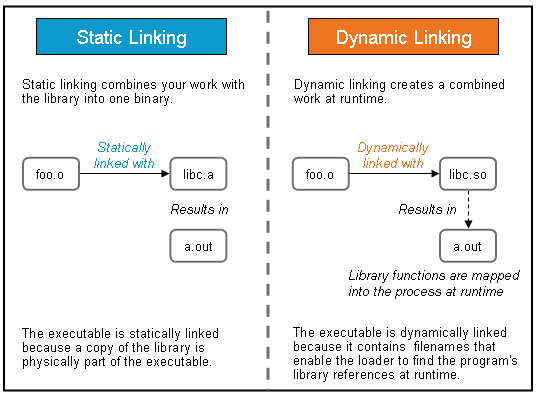
\includegraphics[width=1\textwidth]{images_pfe/sharedlibraryvsstatic.png}
  \caption{Bibliothèque statique vs partagée}
  \label{fig:staticsharedl}
\end{figure}

\paragraph{Bibliothèques statiques vs partagées}
\begin{enumerate}
  \item \textbf{Bibliothèques statiques} :  
    Les bibliothèques statiques sont des archives de routines (\texttt{libfoo.a}) dont les routines nécessaires sont extraites et \textbf{liées directement} dans l’exécutable.  
  \item \textbf{Bibliothèques partagées (dynamiques)} :  
    Les bibliothèques partagées (\texttt{libfoo.so}) sont chargées une seule fois en mémoire virtuelle, puis \textbf{partagées} par tous les programmes qui les utilisent. Elles sont plus économes en espace.\\
\end{enumerate}





\textbf{Exemple d'un exécutable lié statiquement : Hello World en FASM (Flat Assembleur)}

\begin{figure}[H]
  \centering
  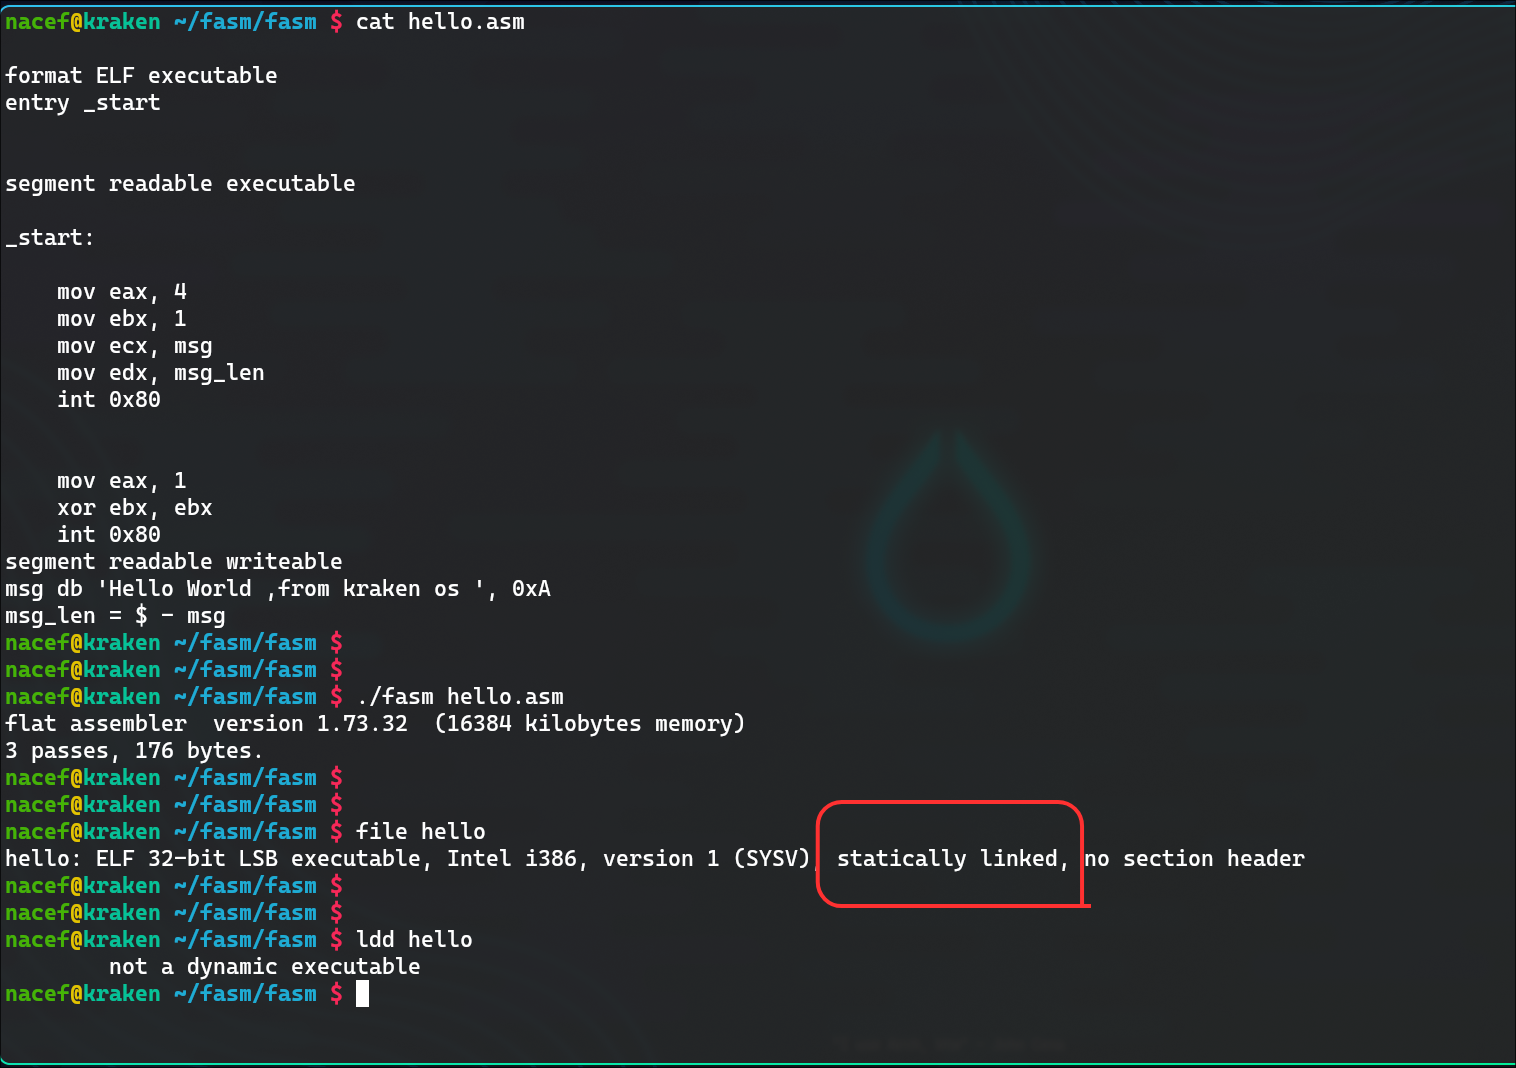
\includegraphics[width=1\textwidth]{images_pfe/staiclulinkedoff.png}
  \caption{Exécutable lié statiquement }
  \label{fig:staticsharedl}
\end{figure}
\clearpage

\textbf{Exemple d'un exécutable lié dynamiquement : Hello World en C }
\begin{figure}[H]
  \centering
  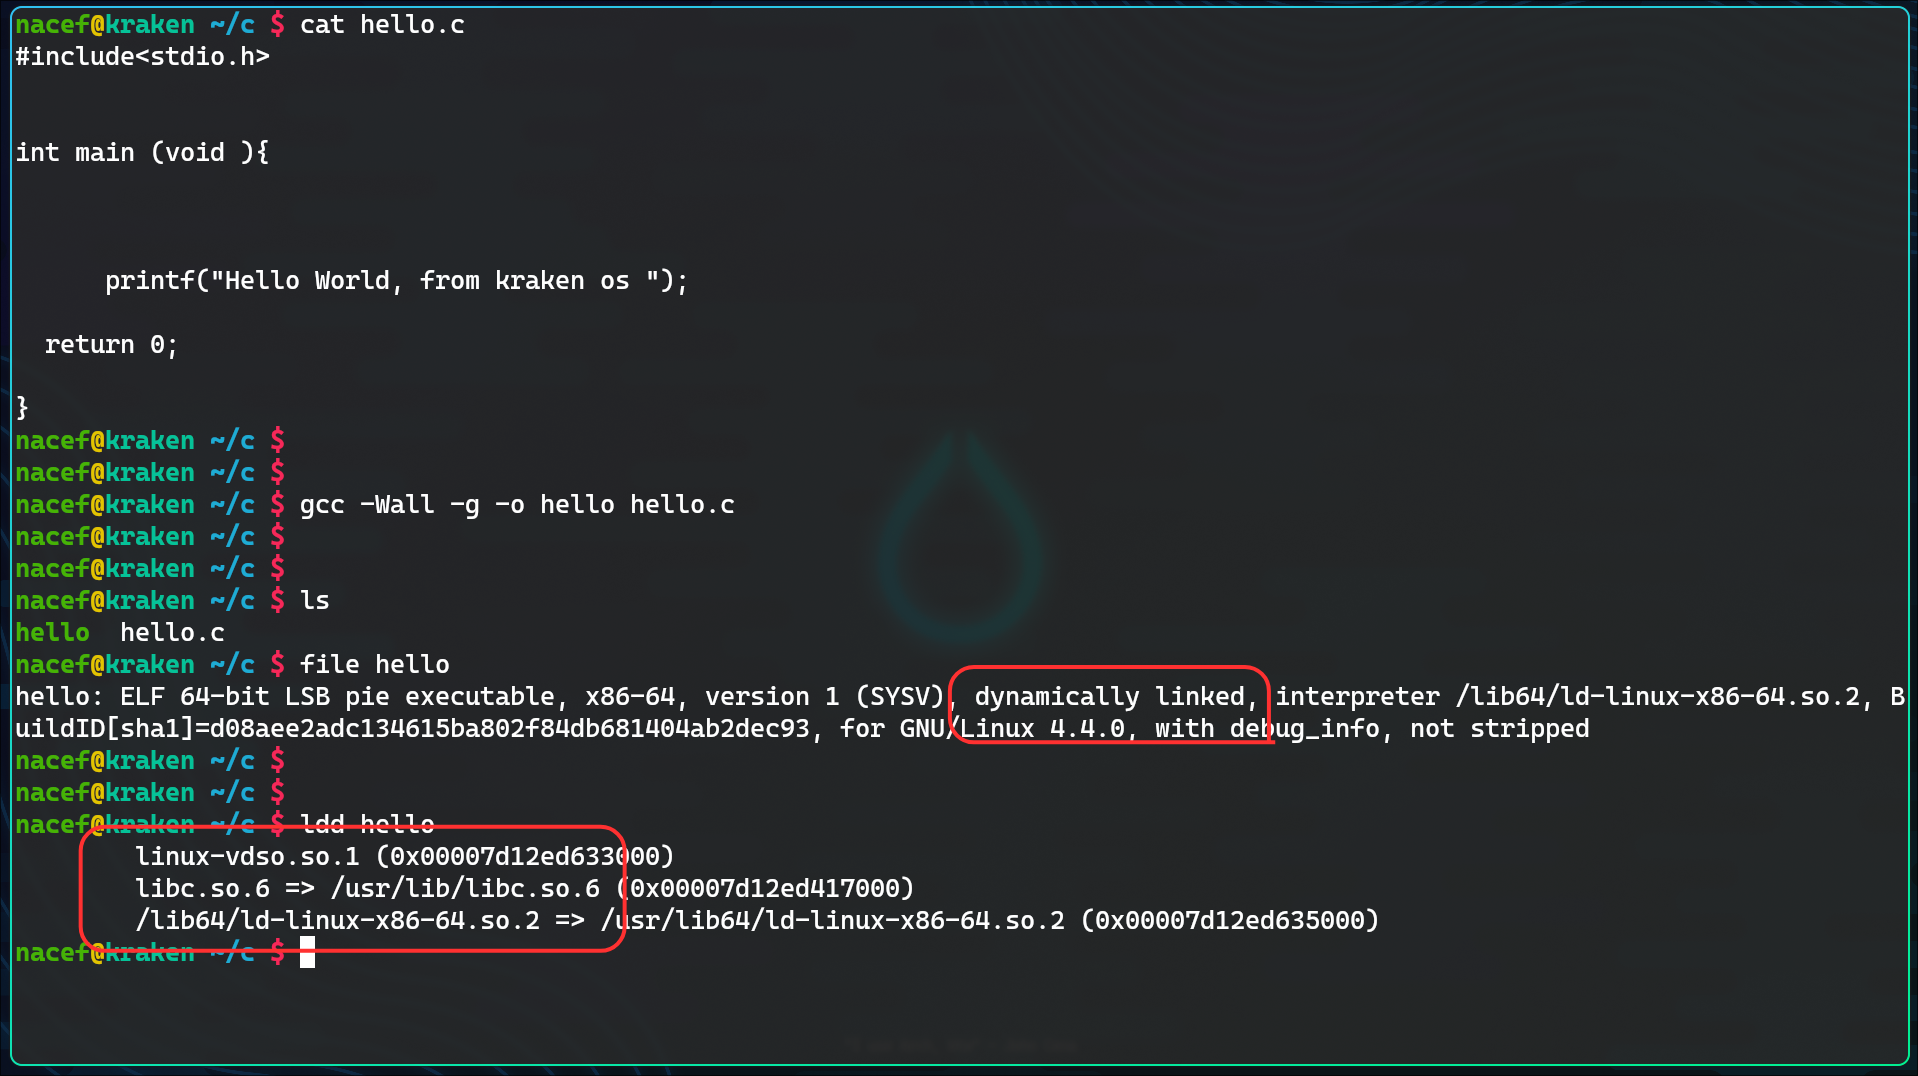
\includegraphics[width=1\textwidth]{images_pfe/dynamiclinkedoff.png}
  \caption{Exécutable lié dynamiquement }
  \label{fig:staticsharedl}
\end{figure}





\paragraph{Remarque}  
En général, les mainteneurs développent ces paquets pour une distribution spécifique (Arch, Debian, etc.). Pour les adapter à  notre distribution, il est parfois nécessaire d’appliquer des patches ou de modifier les chemins dans le code source, car l’emplacement des bibliothèques peut varier d’une distribution à l’autre.  \\
Par exemple, si un paquet s’attend à trouver la bibliothèque \texttt{libX} dans \texttt{/lib} mais que nous l’installons dans \texttt{/usr/lib}, il faudra créer un lien symbolique ou ajuster le chemin de recherche durant le build.  Ce problème est appelé \textbf{erreurs de liaison} (Link Errors)






\section{Qu’est‑ce que la compilation à partir des sources ?}
\label{subsec:compilation-sources}


Un système d’exploitation open‑source est le fruit de l’intelligence collective ; chaque ligne de code est accessible et modifiable. L’installation à partir des sources requiert donc de parcourir les sources de chaque paquet et de les compiler soi‑même pour générer les exécutables, la documentation, les bibliothèques, etc.

Généralement, cette étape de compilation s’effectue en utilisant le \textbf{système de build} propre à chaque paquet.

\subsection{Qu’est‑ce qu’un système de build ?}
\label{sssec:definition-buildsystem}

Un \emph{système de build} est l’outil ou l’ensemble d’outils orchestrant la configuration, la compilation, le lien et l’installation des sources. Parmi les plus courants :

\begin{table}[H]
    \centering
    \begin{tabular}{|c|c|p{8cm}|}
        \hline
        \textbf{Logo} & \textbf{Outil} & \textbf{Fonction principale} \\
        \hline
        
\includegraphics[width=0.8cm]{images_pfe/make.png} & Make & Le plus ancien et basique, utilise des Makefiles. \\
        \hline
        
\includegraphics[width=0.8cm]{images_pfe/GNU-Autoconf-768x288.jpg} & Autotools & Traditionnel pour projets open source, gère la compilation croisée. \\
        \hline
        
\includegraphics[width=0.8cm]{images_pfe/zig.png} & Zig & Outil intégré à Zig (compilation C/C++ possible). \\
        \hline
        
\includegraphics[width=0.8cm]{images_pfe/meson_logo.png} & Meson & Alternative moderne et rapide à CMake/Autotools. \\
        \hline
        
\includegraphics[width=0.8cm]{images_pfe/ninja.jpeg} & Ninja & Outil bas niveau, très rapide, utilisé comme backend pour CMake/Meson. \\
        \hline
    \end{tabular}
    \caption{Principaux systèmes de build}
    \label{tab:build_tools_logos}
\end{table}


%------------------------------------------------
\subsection{Étapes générales de compilation}
\label{sssec:etapes-compilation}

Lors de la construction du système, nous compilons des dizaines de bibliothèques, paquets, etc. Il est donc nécessaire de comprendre comment fonctionne le processus de compilation :

\begin{enumerate}
  \item \textbf{Collecte d’informations}  
    Lire la documentation officielle (wiki, dépôt GitHub/GitLab) pour connaître les dépendances et les options de compilation.\\
    

  \item \textbf{Récupération du code source}  
    Télécharger l’archive (\texttt{.tar.gz}, \texttt{.zip}) à l’aide d’outils tels que \texttt{wget}, \texttt{curl}, ou cloner depuis le dépôt GitLab/GitHub officiel.  
   
    Vérifier ensuite l’intégrité de l’archive (car le téléchargement peut être interrompu ou corrompu),\\ 
     puis l’extraire  et contrôler son contenu (généralement les fichiers du système de build \textcolor{blue}{\ref{fig:makefileexemple}}  ).\\

 \item \textbf{Configuration}  
    À cette étape, le système de build vérifie la présence des bibliothèques, paquets et outils requis, puis active les options souhaitées.  \\

    \textbf{Remarque :} les options de configuration sont très délicates et importantes, car chaque paquet dépend des autres. Il convient donc de se poser deux questions après la configuration de chaque paquet :
    \begin{enumerate}[label=\arabic*)]
      \item Quelle est la configuration nécessaire pour assurer le bon fonctionnement de ce paquet ?
      \item Quelles options doivent être activées maintenant pour que les futurs paquets, qui dépendent de celui-ci, puissent utiliser correctement ses fonctionnalités ?
    \end{enumerate}


    \medskip
    \noindent\textbf{Exemple pratique :} \\ 
    LLVM est un compilateur backend qui gère l’IR (Intermediate Representation). Pour le compiler, il faut construire Clang  (runtime LLVM) d abord  \textbf{avec le support de}  \texttt{compiler-rt} :

    \begin{verbatim}
cmake \
  -DLLVM_ENABLE_PROJECTS="clang;compiler-rt"
    \end{verbatim}
   %Pour plus de détails sur les configurations avec des exemples , voir la section~\hyperref[sec:config-packages]{\textcolor{blue}{\ref*{sec:config-packages}}} de l'annexe.
    
  \item \textbf{Compilation}  
    Après configuration, nous lancer la construction des binaires via le
système de build 

  \item \textbf{Tests (facultatif):}  
     Generalement,après compilation nous tester le paquet, surtout s’il est critique
   
  
\item \textbf{Installation:}  
   installer les fichiers dans l’arborescence cible 

  \item \textbf{Post-configuration (documentation):}  
    Après installation, vous pouvez ajouter des étapes d'installation de documentation ou de génération de fichiers de configuration. 

  \item \textbf{Nettoyage et désinstallation:}  
    Supprimer les fichiers temporaires et le répertoire de
build, tout en conservant l’archive source pour d’éventuelles recompilations.
\end{enumerate}
\clearpage






\textbf{Exemple de fichier Makefile utilisé par le système de build \texttt{make}}\\
Nous présentons ici un Makefile minimal pour le package \texttt{construire\_graphe}, un outil simple écrit en C permettant de générer et visualiser des graphes. Chaque section du Makefile correspond à une étape du processus de compilation standard.

\begin{itemize}
  \item \textbf{Fonctionnalités clés} :
  \begin{itemize}
    \item Construction de graphes via un algorithme implémenté en C
    \item Affichage clair des résultats dans le terminal
    \item Système d’aide intégré pour guider l’utilisateur
  \end{itemize}

  \item \textbf{Composants principaux} :
  \begin{itemize}
    \item \texttt{construire\_graphe} : exécutable principal
    \item \texttt{graph.h/graph.c} : bibliothèque de manipulation de graphes
    \item \texttt{helpmenu.sh} : script d’aide interactif
  \end{itemize}
\end{itemize}

\begin{figure}[H]
  \centering
  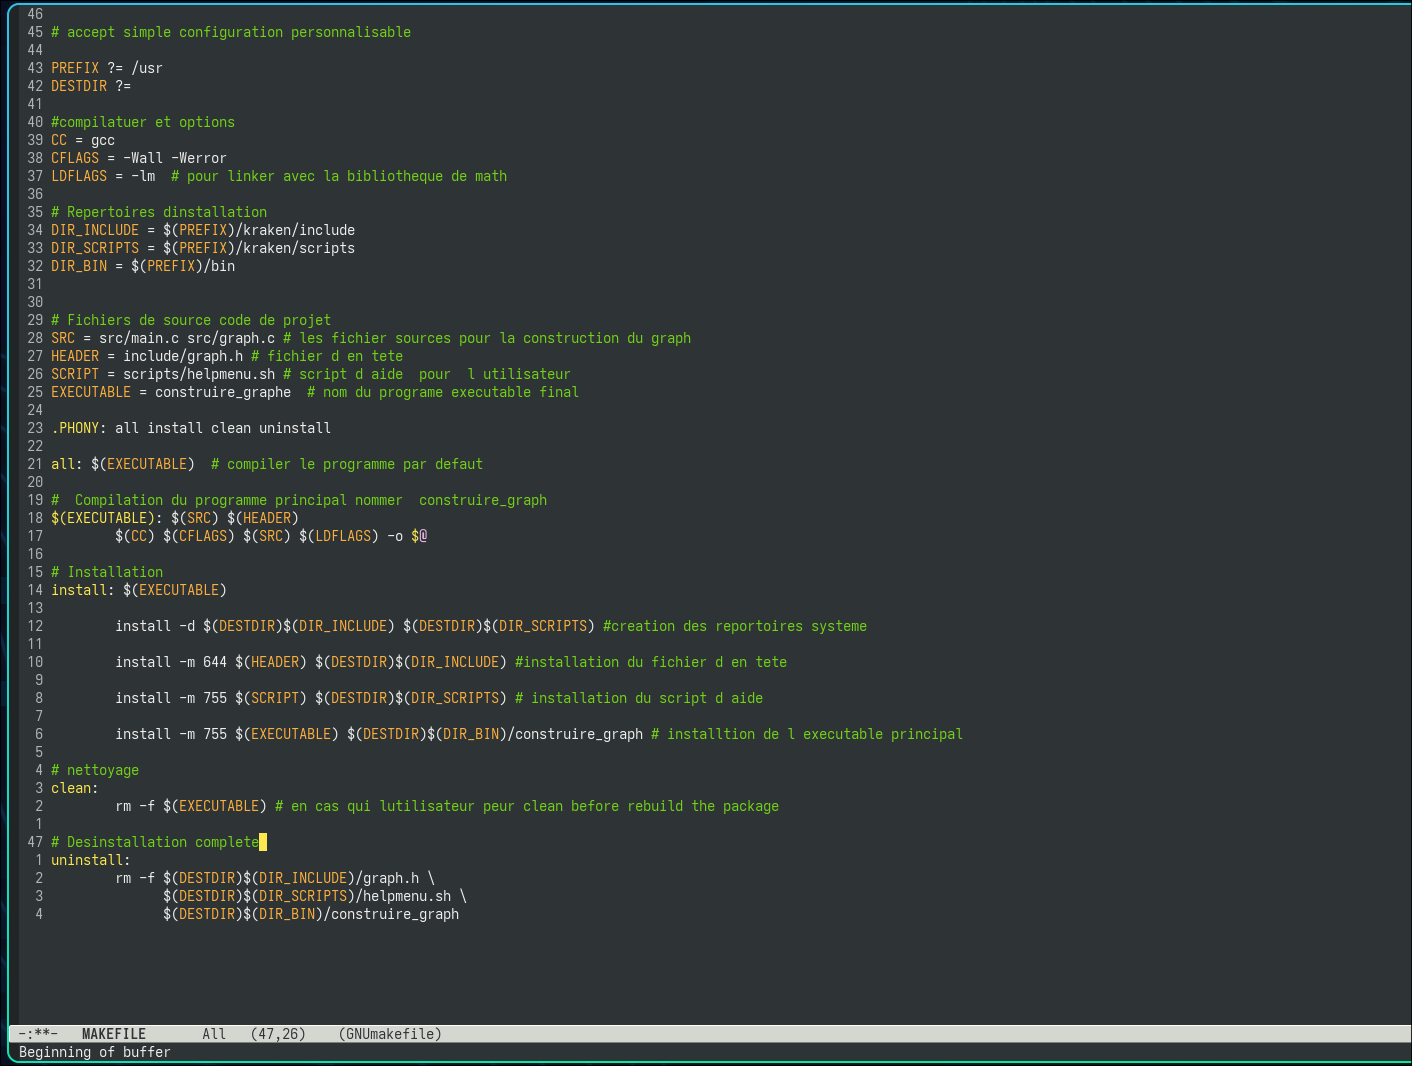
\includegraphics[width=\textwidth]{images_pfe/makefileexemple.png}
  \caption{Exemple de fichier Makefile}
  \label{fig:makefileexemple}
\end{figure}
\clearpage
Le processus de compilation avec \texttt{make} peut être résumé en six étapes clés, illustrées par notre Makefile :

\begin{enumerate}
  \item \textbf{Récupérer le code source de l’outil\\}  
    Par exemple :\\
    \begin{verbatim}
wget https://www.exemple_domain.tn/graph/releases/graph-1.0.1.tar.xz
    \end{verbatim}

  \item \textbf{Extraire l’archive}  
    \begin{verbatim}
tar -xvf graph-1.0.1.tar.xz
    \end{verbatim}

    Exemple de structure du projet :
    \begin{figure}[H]
      \centering
      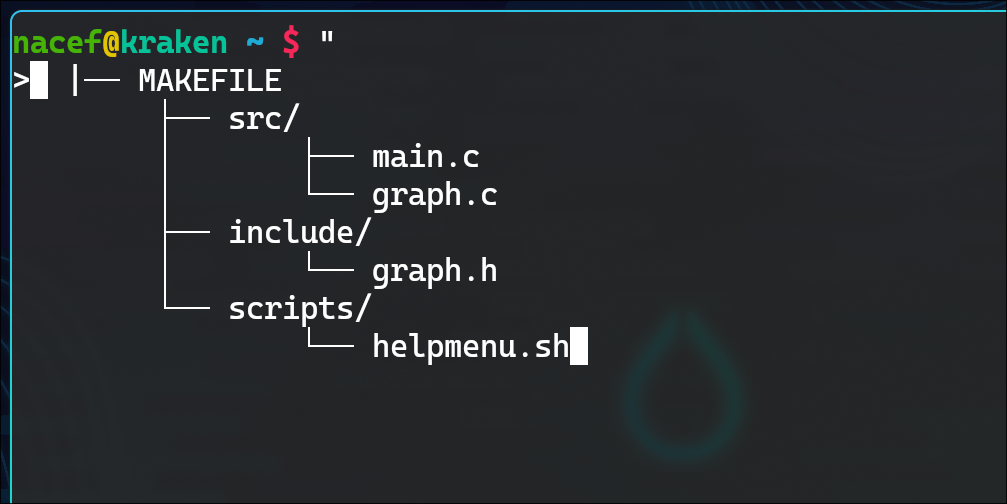
\includegraphics[width=0.7\textwidth]{images_pfe/construire_graph_structure.png}
      \caption{Structure du projet \texttt{construire\_graphe}}
      \label{fig:construire_graph}
    \end{figure}

  \item \textbf{Compilation}  
    \begin{verbatim}
make --DESTDIR=/opt
    \end{verbatim}
    Lorsque vous exécutez \texttt{make}, l’outil cherche la première cible (ici \texttt{all}), constate que \texttt{construire\_graphe} est nécessaire, puis exécute la règle correspondante :  
    \begin{verbatim}
gcc -Wall -Werror src/main.c src/graph.c -lm -o construire_graphe
    \end{verbatim}

  \item \textbf{Installation}  
    \begin{verbatim}
make DESTDIR=/opt install    
    \end{verbatim}
    Cette cible crée d’abord les répertoires d’installation :\\
    \begin{verbatim}
install -d /opt/kraken/include /opt/kraken/scripts

    \end{verbatim}
Puis copie les fichiers avec les permissions adéquates :\\

  \begin{verbatim}

install -m 644 graph.h          /opt/kraken/include
install -m 755 helpmenu.sh      /opt/kraken/scripts
install -m 755 construire_graphe /opt/bin
    \end{verbatim}

  \item \textbf{Nettoyage}  
    \begin{verbatim}
make clean
    \end{verbatim}
    Avec la règle dans le Makefile :
    \begin{verbatim}

clean:
    rm -f construire_graphe
    \end{verbatim}
    Cette cible supprime l’exécutable compilé.

  \item \textbf{Désinstallation}  
    \begin{verbatim}
make uninstall
    \end{verbatim}
    Avec la règle dans le Makefile :
    \begin{verbatim}

uninstall:
    rm -f /opt/kraken/include/graph.h \\
          /opt/kraken/scripts/helpmenu.sh \\
          /opt/bin/construire_graphe
    \end{verbatim}
    Cette cible retire les fichiers installés.
\end{enumerate}

  





   
\textcolor{blue}{Pour plus d’informations sur la compilation des paquets depuis les sources, consultez} \cite{tutoriel_unix}

\section{Qu’est‑ce que le \emph{bootstrap} ?}
\label{subsec:bootstrap}
\begin{figure}[H]
  \centering
  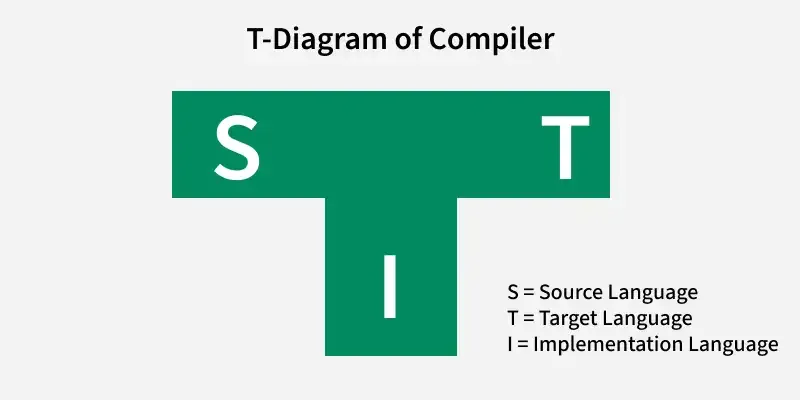
\includegraphics[width=0.85\textwidth]{images_pfe/bootstrap.png}
  \caption{Schéma de l’amorçage d’un compilateur}
  \label{fig:bootstrap}
\end{figure}

Lors de la compilation de paquets à partir des sources, nous rencontrons souvent des problèmes liés à l’amorçage (\emph{bootstrap}).  \\
Le \emph{bootstrap}  permet de compiler un composant dont le compilateur est écrit dans le même langage — et donc non disponible a priori sur la machine de construction. 

\bigskip
\noindent
\textbf{Problème}  
Supposons que l’on veuille construire le langage \texttt{Go}, dont le compilateur  est écrit en la langage  \texttt{Go} lui‑même. Comment produire un exécutable quand aucun compilateur \texttt{Go} n’est encore installé ?

\medskip
\noindent
\textbf{Solution}  
On utilise un \emph{bootstrap} : un binaire pré‑compilé ou un compilateur antérieur sert à générer la première version du compilateur \texttt{Go}. Ce compilateur issu du bootstrap est ensuite utilisé pour compiler la version finale.  \\
Vous pouvez simplement comprendre ce concept comme « compiler un compilateur à l’aide d’un compilateur préexistant pour générer le compilateur définitif ! »\\



Cette méthode générale s’applique à tout langage ou outil dont le compilateur est en auto‑hospitage (\emph{self‑hosting}).( Exemple :langage go,  langage rust , language java ...) \\
\textcolor{blue}{Pour plus d’informations sur auto-hospitage, consultez \cite{bootstrap}}
%-------------------compiler ------------------
\section{Compilateur croisé}
\label{subsec:cross-compiler}

La compilation croisée est utilisée pour construire un compilateur et sa chaîne d’outils pour une machine différente de celle servant à la compilation. \\ 
Simplement pour générer des exécutables qui fonctionneront sur une machine différente de la machine hôte .\\ 
Par exemple, on peut utiliser un cross-compiler installé sur une architecture x86\_64 pour produire des exécutables destinés à l’architecture ARM .

\begin{figure}[!htbp]
  \centering
  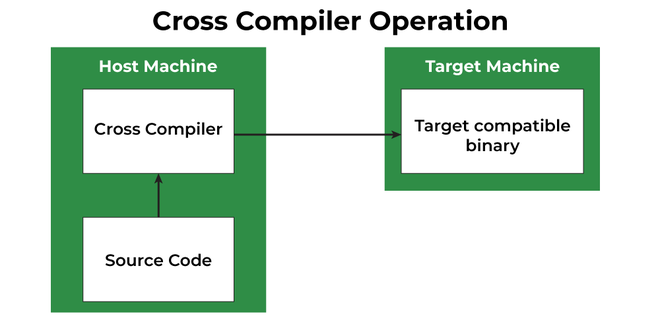
\includegraphics[width=0.85\textwidth]{images_pfe/crosscompiler.png}
  \caption{Compilateur croisé}
  \label{fig:crosscompiler}
\end{figure}

%\subsubsection{Notions clés}
%\begin{itemize}
  %\item \textbf{Build} : machine utilisée pour la compilation.
 % \item \textbf{Host} : machine sur laquelle les programmes compilés seront exécutés.
 % \item \textbf{Target} : architecture cible pour laquelle le code est généré.
%\end{itemize}


%\subsection{Exemple pratique : Canadian Cross}
%La méthode dite « Canadian Cross » se déroule en quatre étapes successives, impliquant trois machines distinctes.

%Nous disposons d'un compilateur natif sur une machine lente (machine A), appelé \texttt{ccA}. Nous disposons également d'une machine rapide (machine B) \textbf{sans compilateur}, et nous souhaitons produire du code pour une troisième machine lente (machine C).\\
%Nous allons construire un compilateur pour la machine C en quatre étapes :

%\begin{table}[!htbp]
 % \centering
 % \caption{Processus de compilation « Canadian Cross »}
 % \label{tab:canadian-cross}
 % \begin{tabular}{|l|l|l|l|p{6cm}|}
 %   \hline
 %   \textbf{Étape} & \textbf{Build}    & \textbf{Host}    & \textbf{Target}  & \textbf{Action}                                      \\
 %   \hline
 %   1              & A          & A                & B                & Compilation de \texttt{cc1}  avec \texttt{ccA} sur A    \\
 %   \hline
    %2              & A                 & B                & C                & Compilation %de \texttt{cc2} à l’aide de \texttt{cc1} sur A                \\
    %\hline
    %3              & B            & C                & C                & Compilation de \texttt{ccC} (natif) avec \texttt{cc2} sur B                \\
   % \hline
   % 4              & C                 & C                & C                & Rebuild et test de \texttt{ccC} avec lui‑même sur C                      \\
   % \hline
  %\end{tabular}
%\end{table}

%Dans cet exemple :
%\begin{itemize}
%  \item \textbf{cc1}, \textbf{cc2} : compilateurs croisés, générant du code pour une autre %architecture.
%  \item \textbf{ccA}, \textbf{ccC} : compilateurs natifs, générant du code pour leur %machine hôte.
%\end{itemize}

%\bigskip
%\noindent
\textbf{Remarque :} dans le cas de \textsc{notre distribution}, la machine hôte  et la machine cible(kraken os) sont identiques (même architecture x86-64).\\
\textbf{Pourquoi utiliser alors un compilateur croisé ?}\\
Tout simplement pour \textbf{l’isolation  :}  car  tout ce qui est compilé en croisé ne peut pas dépendre de l’environnement hôte.\\
En effet, si nous compilons nos paquets système à l’aide du compilateur du système hôte, les outils et les exécutables sont liés dynamiquement à des bibliothèques présentes sur l’hôte,Donc Les outils générés resteront dépendants de cet environnement. Ainsi, lorsque nous effectuons un chroot ou que nous démarrons notre système, tous ces exécutables produits ne fonctionneront pas

\medskip
\noindent
\textbf{Solution :}  
Nous mettrons en œuvre un « faux » cross‑compiler. Cette approche sera détaillée dans le  Section~\textcolor{blue}{\ref{subsec:build-cross}}.\\

\textcolor{blue}{Pour plus d’informations sur le compilateur croisé, consultez \cite{lfs_book} des pages 39 à 43.}  
\section{Conclusion }

Compiler un logiciel à partir des sources reste une tâche exigeante, souvent perçue comme laborieuse en raison de son \textbf{coût temporel} et de sa \textbf{complexité technique} . La configuration des paquets, les dépendances imbriquées et la compilation de projets massifs (GCC, Qt6, KDE, LLVM, Mesa, ou le noyau Linux) peuvent monopoliser des heures de calcul, même sur des machines puissantes dotées de 8 cœurs CPU.

C’est précisément pour simplifier cette démarche que les grandes distributions Linux ont développé des gestionnaires de paquets ,  mais au fait, \textbf{qu’est-ce qu’un gestionnaire de paquets ? Comment fonctionne-t-il ? }\\

C’est ce que nous découvrirons dans le prochain chapitre !
\chapter{Le gestionnaire de paquets }
\minitoc
\clearpage

\label{sec:kraken-pkg}
\section{Introduction}
Un gestionnaire de paquets est un outil  permettant d’automatiser les processus d’installation, de mise à jour et de suppression de paquets sur un système Linux. 

Malheureusement, le mécanisme de gestion des paquets n’est pas un aspect purement théorique. En pratique, chaque grande distribution conçoit son propre gestionnaire de paquets, selon une philosophie qui lui est propre.\\
À ce stade, il est donc important de comprendre que nous devons inventer un nouveau gestionnaire de paquets conçu et développé entièrement à partir de zéro, sans s’appuyer sur
un autre gestionnaire existant

L’objectif du gestionnaire de paquets \textsc{Kraken} est de fournir une solution à la fois simple et efficace pour l’installation, la mise à jour, la configuration et la suppression des logiciels. Il prend en charge les dépendances, la gestion des versions, ainsi que toutes les tâches complexes afin de faciliter la gestion des programmes.



%\subsection{Fonctionnalités du gestionnaire de paquets sous Linux}
%\label{subsec:kraken-fonctions}

%\begin{itemize}
 % \item \textbf{Installation}  
  %  Permet d’installer des paquets depuis des dépôts distants . Gère automatiquement les dépendances
  %\item \textbf{Résolution de dépendances}  
  %  Analyse les besoins de chaque paquet et récupère automatiquement les paquets requis.
  %\item \textbf{Mise à jour (upgrade)}  
  %  Met à jour les paquets installés vers leurs dernières versions, assurant ainsi la sécurité et la fraîcheur du système.
  %\item \textbf{Suppression}  
  %  Désinstalle les paquets et leurs dépendances obsolètes, sans laisser de fichiers orphelins.
  %\item \textbf{Interrogation (query)}  
  %  Fournit des commandes pour lister les paquets installés, les mises à jour disponibles et les détails de %chaque paquet.
%\end{itemize}



\section{ Architecture du  la gestionnaire de paquets }


 


\begin{figure}[H]
  \centering
  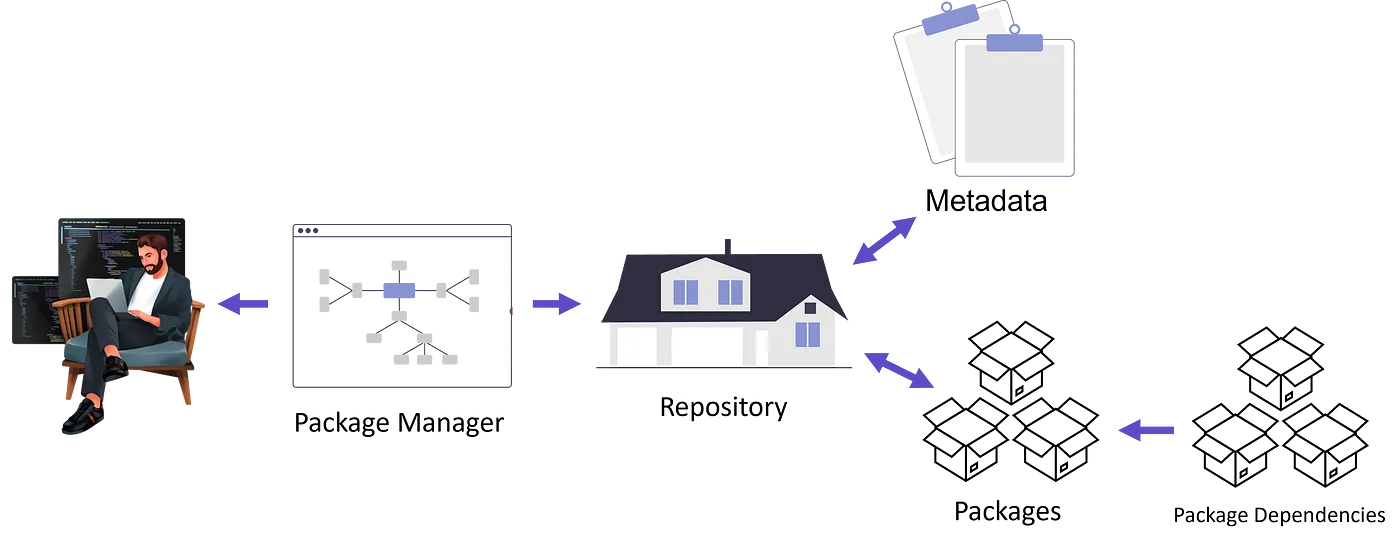
\includegraphics[width=0.85\textwidth]{images_pfe/packagemanager.png}
  \caption{ Architecture gestionnaire de paquets }
  \label{fig:packagemanager}
\end{figure}


 Cette figure illustre la manière dont nous avons conçu notre gestionnaire de paquets. 
 Le premier composant de Kraken est le \textbf{dépôt} (Repository) , où sont stockées les métadonnées des paquets. Chaque paquet est décrit par un fichier \textbf{pkgbuild.kraken}(metadata), qui définit la procédure d'installation du paquet sur notre  à l'aide du gestionnaire de paquets Kraken. \\
 Le deuxième composant correspond aux \textbf{outils du gestionnaire de paquets}, qui permettent de récupérer, interroger et installer les paquets depuis le dépôt vers le système. 

Avant de commencer à développer le gestionnaire de paquets \textsc{Kraken}, il est essentiel de comprendre un problème majeur connu sous le nom de \textbf{« dependency hell »} (l’enfer des dépendances).

\section{Qu’est‑ce qu’une dépendance de paquet ?}
\label{subsec:dependency}

Une dépendance de paquet est l’ensemble des autres paquets, bibliothèques ou outils requis pour qu’un paquet puisse s’installer et fonctionner correctement. Pour installer un paquet, il faut résoudre automatiquement toutes ses dépendances dans le bon ordre. 

On peut visualiser ce processus comme un graphe orienté : chaque nœud représente un paquet, et chaque arc pointe vers un paquet dont il dépend.  

\begin{figure}[H]
  \centering
  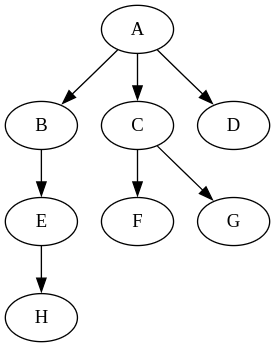
\includegraphics[width=0.5\textwidth , height=10cm]{images_pfe/genralgraphexemple.png}
  \caption{Exemple de graphe de dépendances}
  \label{fig:exempledepndencygraph}
\end{figure}


Pour installer le paquet \texttt{A} :
\begin{enumerate}
  \item Il faut d’abord installer \texttt{B}, \texttt{C} et \texttt{D}.
  \item Pour \texttt{B}, on doit installer \texttt{E}, lui‑même dépendant de \texttt{H}.
  \item Une fois \texttt{B}  installés, on revient au sous‑graphe de \texttt{C} et on installe \texttt{F} et \texttt{G}.
\end{enumerate}

Cette résolution suit en général un algorithme de \textbf{parcours en profondeur} (DFS) du graphe de dépendances.  

Cependant, dans la pratique, le graphe peut être très vaste (des dizainess de paquets) et contenir  des cycle. Il faut alors mettre en place des stratégies d’optimisation (caching, détection de cycles, etc.). Tous ces enjeux sont regroupés sous le terme \textbf{« enfer des dépendances »} (Dependency Hell).


\subsection{Premier problème : dépendances circulaires}
\label{subsec:circular-dependencies}

Une dépendance circulaire survient lorsqu’un paquet A dépend d’un paquet B, qui lui-même dépend de A. Cette situation bloque la résolution automatique des dépendances, car ni A ni B ne peut être installé en premier sans l’autre.

\begin{figure}[H]
  \centering
  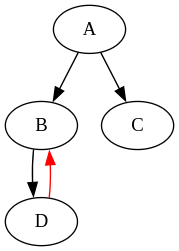
\includegraphics[width=0.3\textwidth, height=8cm]{images_pfe/CERCULARDEP.png}
  \caption{Exemple simple de dépendance circulaire}
  \label{fig:circular-dep}
\end{figure}



Sur la figure~\textcolor{blue}{\ref{fig:circular-dep}}, pour installer \texttt{B}, il faut d’abord installer \texttt{D}, qui dépend de \texttt{B}, bouclant ainsi le processus.

\paragraph{Cas d’usage réel : outils multimédia}
Considérons deux paquets :
\begin{itemize}
  \item \textbf{DocumentConverter} : convertit des documents (PDF → Word, etc.) et nécessite \texttt{FileViewer} pour prévisualiser les fichiers convertis.
  \item \textbf{FileViewer} : affiche des documents (PDF, Word, ODT, etc.) et nécessite \texttt{DocumentConverter} pour convertir les \textbf{formats non pris en charge}.
\end{itemize}

\begin{figure}[H]
  \centering
  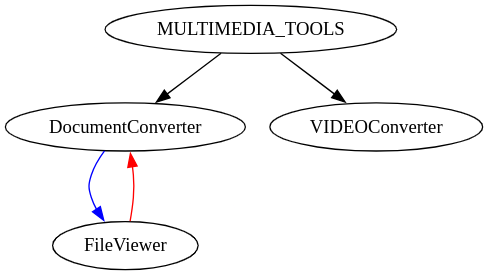
\includegraphics[width=0.5\textwidth]{images_pfe/depcycleexemple.png}
  \caption{Boucle de dépendance entre \texttt{DocumentConverter} et \texttt{FileViewer}}
  \label{fig:depcycle-multimedia}
\end{figure}



\subsubsection*{Stratégie de résolution}
Pour casser la boucle de dépendances, on procède en plusieurs étapes :
\begin{enumerate}
  \item \textbf{Installation initiale de FileViewer (minimal)}  
    Compiler et installer \texttt{FileViewer} \textbf{sans} le support de conversion.
  \item \textbf{Installation de DocumentConverter}  
    Compiler et installer \texttt{DocumentConverter}, qui s’appuie sur le FileViewer minimal.
  \item \textbf{Recompilation de FileViewer}  
    Recompiler \texttt{FileViewer} en activant le support de \texttt{DocumentConverter}.
  \item \textbf{Installation finale de FileViewer complet}  
    Installer la nouvelle version de \texttt{FileViewer} avec toutes les fonctionnalités.
\end{enumerate}

Cette méthode garantit que chaque paquet et ses dépendances sont disponibles au moment opportun, évitant ainsi l’« enfer des dépendances » engendré par les boucles circulaires. 



\subsection{Deuxième problème : conflit de dépendances}
\label{subsec:dependency-conflict}

Un conflit de dépendances survient lorsque deux paquets, ou plus, requièrent la même bibliothèque ou le même composant, mais chacun spécifie une version différente. Par exemple, sur la figure~\textcolor{blue}{\ref{fig:dependency-conflict}} :

\begin{figure}[H]
  \centering
  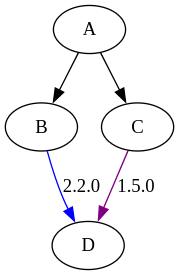
\includegraphics[width=0.3\textwidth, height=5cm]{images_pfe/dpendencyconfligt.png}
  \caption{Exemple de conflit de dépendances }
  \label{fig:dependency-conflict}
\end{figure}

Ici, \texttt{B} dépend de \texttt{D} en version 2.2.0, alors que \texttt{C} exige la version 1.5.0. Le gestionnaire doit alors choisir :

\begin{itemize}
  \item Installer la version la plus récente (2.2.0), au risque de casser \texttt{C}.
  \item Installer la version la plus ancienne (1.5.0), au risque de manquer des correctifs ou fonctionnalités pour \texttt{B}.
  \item Installer simultanément les deux versions, .  au risque de conflit dans le systeme
\end{itemize}

\subsubsection*{Stratégies de résolution}

Malheureusement, ce problème est, pour moi, un problème non résolu en informatique. J'ai effectué de nombreuses recherches pour tenter de trouver une solution, mais chaque gestionnaire de paquets essaie seulement de le contourner sans réellement parvenir à une solution pratique.\\ En général, ils se contentent d'afficher un message à l'utilisateur pour l'informer qu’un conflit existe entre deux ou plusieurs paquets. C’est également l’approche que nous avons choisie. Par exemple, le gestionnaire de paquets \texttt{pacman} de archlinux ou encore \texttt{xbps} de Void Linux adoptent cette stratégie.




\section{Pourquoi avons-nous besoin d’un mécanisme de suivi des métadonnées des paquets ?}
\label{subsec:suivi-fichiers}

Dans un système Linux, l’installation d’un paquet répartit ses fichiers sur de nombreux emplacements :
\begin{itemize}
  \item Binaires : \texttt{/usr/bin}, \texttt{/usr/local/bin}, etc.  
  \item Bibliothèques : \texttt{/lib}, \texttt{/usr/lib}, \texttt{/lib64}, etc.  
  \item En-têtes : \texttt{/usr/include}, etc.  
  \item Fichiers de configuration : \texttt{/etc}.  
  \item Documentation : \texttt{/usr/share/doc}, \texttt{/usr/share/man}, etc.  
  \item Éléments supplémentaires : \texttt{/opt}, \texttt{/var}, etc.  
\end{itemize}

Sans mécanisme de suivi, désinstaller proprement un paquet devient fastidieux : il faudrait rechercher manuellement chacun de ses fichiers dans tout le système, ce qui est impraticable quand on gère des centaines de milliers de fichiers.

\textbf{Notre solution :} développer un mécanisme de « fausse installation ». Ce mécanisme doit générer des fichiers de métadonnées contenant tous les chemins des fichiers et répertoires créés ou modifiés lors de l’installation du paquet. \textbf{Nous détaillerons cette approche dans le section} \textcolor{blue}{\ref{subsecc:fakeinstall}} .
\section{Conclusion}
Le gestionnaire de paquets est l'un des composants les plus complexes et cruciaux d'une distribution Linux. Il nécessite une approche rigoureuse , surtout lorsqu'il s'agit de construire les paquets à partir des sources. \\
En effet, une simple erreur dans ce composant peut compromettre le système entier, le rendant inutilisable.



\clearpage
\chapter{Architecture noyau , bootloader et  system V}
\minitoc
\clearpage
\section{Noyau et choix des modules}
\label{subsec:noyau-modules}

Le noyau Linux est l’élément central d’un système d’exploitation, responsable de la gestion des ressources matérielles et de l’interaction avec le matériel. Le projet Linux est l’un des plus importants projets open-source au monde, rassemblant des milliers de contributeurs et générant des millions de lignes de code modifiées à chaque version. \\ 
Le mainteneur principal : Linus Torvalds.


Avant de configurer et compiler le noyau, il est essentiel de comprendre ses composants fondamentaux (voir figure~\textcolor{blue}{\ref{fig:kernel-arch}}) :

\begin{figure}[H]
  \centering
  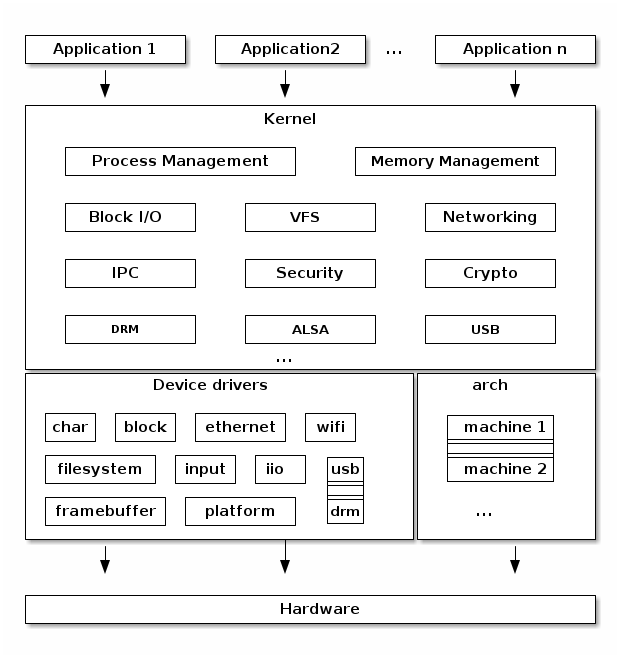
\includegraphics[width=0.85\textwidth]{images_pfe/kernelarchitecture.png}
  \caption{Architecture générale du noyau Linux}
  \label{fig:kernel-arch}
\end{figure}

\begin{description}
  \item[1. Architecture (\texttt{arch})]  
    Contient le code spécifique aux architectures matérielles (x86, ARM, MIPS, PowerPC, IBM S/390, etc.), parfois subdivisé en code machine spécifique.
  \item[2. Pilotes de périphériques (Device Drivers)]  
    Mise en œuvre d’un modèle unifié pour gérer les périphériques : détection, état, bus d’attache et liaison avec le pilote approprié.
  \item[3. Gestion des processus (Process Management)]  
    Création, ordonnancement et terminaison des processus. Implémentation des appels \texttt{fork()}, \texttt{exec()}, \texttt{wait()} et des threads POSIX via la structure \texttt{task\_struct}.
  \item[4. Gestion de la mémoire (Memory Management)]  
    Allocation et libération de la mémoire physique et virtuelle : pagination, swap, \texttt{mmap()}, \texttt{brk()}, allocateurs SLAB et \texttt{vmalloc}.
  \item[5. Gestion du Block I/O (Block I/O Management)]  
    Création et ordonnancement des requêtes d’E/S sur périphériques bloc : RAID logiciel, LVM, fusion et tri des requêtes, planification par ordonnanceurs d’I/O.
\end{description}


\bigskip
L’un des aspects les plus enthousiasmants d’un système d’exploitation moderne — protection, concurrence, virtualisation, allocation de ressources et stockage fiable — est qu’ils se retrouvent aujourd’hui dans de nombreux domaines de l’informatique, au‑delà des seuls noyaux. Il est impossible de concevoir des systèmes informatiques résilients, sécurisés et flexibles sans appliquer ces concepts fondamentaux


\textcolor{blue}{Pour plus d’informations sur larchitecture du noyau linux, consultez \cite{Linux_kernel_course} }  
%\begin{figure}[H]
%  \centering
 % 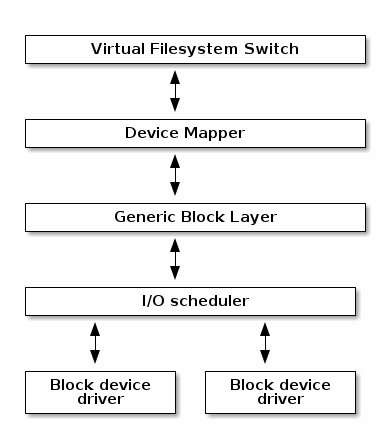
\includegraphics[width=0.85\textwidth]{images_pfe/iomanagmemnt.png}
%  \caption{Architecture du sous‑système Block I/O}
%  \label{fig:io-management}
%\end{figure}
\section{Configuration du noyau}
%\textcolor{red}{TBD: add figure and ressources}
Dans le noyau Linux, il existe deux types de configurations principales :

\begin{enumerate}
  \item \textbf{Intégrée au noyau (built-in)}

  Lorsqu'une option est activée en tant qu’élément intégré (\texttt{built-in}), cela signifie qu’elle est compilée directement dans l’image binaire du noyau (\texttt{vmlinuz}).

  \textbf{Caractéristiques :}
  \begin{itemize}
    \item \textbf{Toujours disponible} : Pas besoin de la charger manuellement, elle fait partie du noyau dès le démarrage.
    \item \textbf{Pas de surcharge à l’exécution} : Exécution plus rapide, car le code est déjà en mémoire.
    \item \textbf{Critique pour le démarrage} : Les pilotes matériels essentiels (ex. : contrôleurs de disque, systèmes de fichiers) doivent être intégrés si nécessaires pendant les premières étapes du démarrage .
  \end{itemize}

  \item \textbf{Modules chargeables (Loadable Kernel Modules)}

  Les fonctionnalités marquées comme \texttt{m} (module) sont compilées séparément sous forme de fichiers objets \texttt{.ko} (Kernel Object), stockés dans \texttt{/lib/modules}.

  \textbf{Caractéristiques :}
  \begin{itemize}
    \item \textbf{Chargés à la demande} : Manuellement via \texttt{modprobe}, ou automatiquement via \texttt{udev}.
    \item \textbf{Utilisation mémoire réduite} : Les modules ne sont chargés que lorsqu’ils sont nécessaires.
    \item \textbf{Flexibilité de mise à jour} : Les modules peuvent être recompilés ou rechargés sans nécessiter de redémarrage du système.
  \end{itemize}
\end{enumerate}




Pour \textsc{Kraken OS}, nous avons retenu le noyau Linux \texttt{6.10.5}, garantissant un équilibre entre stabilité et fonctionnalités récentes. Nous avons activé uniquement les modules nécessaires aux architecture cible  x86\_64, et désactivé les options optionnelles afin de réduire l’empreinte mémoire et d’optimiser les performances. 


\section{Systèmes d'initialisation : System V et SystemD}
\label{sssec:sysv}

Il existe deux principaux types de systèmes d'initialisation : \textbf{SystemD} et \textbf{System V}. \\
System V est plus ancien. Il s'appuie sur un petit programme appelé \texttt{init}, dont le rôle est de configurer les processus de base du système et d'exécuter un script principal (nommé \texttt{rc}). Ce script orchestre une série de scripts secondaires destinés à initialiser les services système.

SystemD est un système plus moderne, conçu pour permettre \textbf{un démarrage plus rapide} et une \textbf{meilleure gestion des dépendances}.

\begin{itemize}
    \item \textbf{SystemD} utilise des fichiers \texttt{.service} pour contrôler les processus.
    \item \textbf{System V} repose sur des scripts shell situés dans \texttt{/etc/init}.
\end{itemize}

\bigbreak
Il est clair que SystemD est plus moderne et adopté par la majorité des distributions récentes. Toutefois, il est également \textbf{plus complexe}, notamment dans sa \textbf{gestion des dépendances}. \\
C’est pourquoi nous avons choisi d’utiliser System V — tout simplement pour sa simplicité — car, à ce stade, notre objectif principal était d’obtenir un système bootable.

Nous ignorions alors que ce choix constituerait une \textbf{erreur stratégique}, car il a engendré plusieurs inconvénients :
\begin{itemize}
    \item un temps de démarrage plus long,
    \item un traitement séquentiel des services,
    \item une complexité accrue lors de l’ajout de nouveaux scripts.
\end{itemize}

Nous travaillerons dur dans la prochaine version de la distribution pour résoudre ce problème en utilisant SystemD à la place de System V.

%\begin{itemize}
 %   \item \textbf{Temps de démarrage allongé} : Une instance basique de notre système démarre en 8 à 12 secondes (mesurées du premier message du noyau jusqu'à l'invite de connexion).
    
  %  \item \textbf{Traitement séquentiel} : Un retard dans un processus  bloque l'ensemble du démarrage.
    
   % \item \textbf{Complexité d'ajout} : L'ajout de nouveaux services nécessite une planification manuelle de l'ordre d'exécution.
%\end{itemize}

\textcolor{blue}{Pour une analyse détaillée de SystemD vs System V, voir \cite{systemV_systemD}.}


\section{Qu'est-ce qu'un bootloader ?}

Il existe deux grands chargeurs d'amorçage (bootloaders) pour les systèmes Unix : \textbf{GRUB} et \textbf{Syslinux}.  \\
Dans \textsc{Kraken OS}, nous avons choisi d’utiliser \textbf{GRUB} pour démarrer le système depuis le disque, et \textbf{Syslinux} pour l’intégration dans le fichier ISO bootable.  

%Nous parlerons de \textbf{Syslinux} dans les chapitres suivants, mais concentrons-nous maintenant sur \textbf{GRUB}.



\medskip
\noindent
En bref, un \textit{bootloader} est le premier programme logiciel exécuté au démarrage d’un ordinateur. Il est responsable du chargement et du \textbf{transfert de contrôle} vers le noyau du système d’exploitation.  
Ce dernier se charge ensuite de l’initialisation complète du système.

Pour visualiser ce processus, reportez-vous à la figure suivante qui montre un schéma simplifié du démarrage :

\begin{figure}[H]
  \centering
  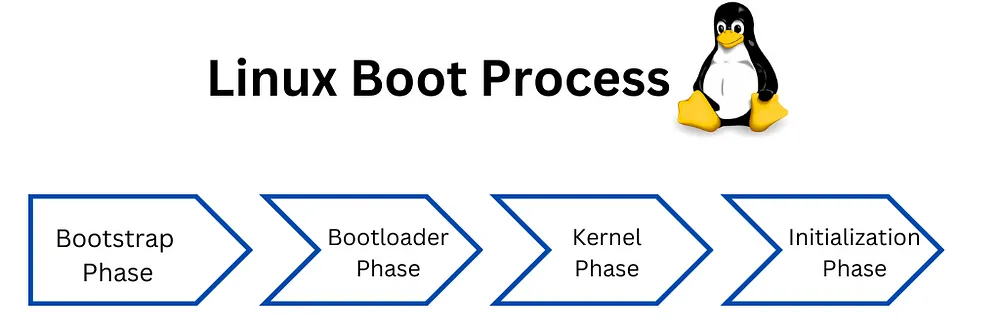
\includegraphics[width=0.85\textwidth]{images_pfe/simplebootprocess.png}
  \caption{Processus de démarrage simplifié}
  \label{fig:botprocess}
\end{figure}



\bigskip
\noindent
GRUB adopte une syntaxe particulière pour désigner les disques et leurs partitions.  
Cette notation suit le format \texttt{(hdX,Y)}, où :
\begin{itemize}
  \item \texttt{X:} représente le numéro du disque dur
  \item \texttt{Y:} désigne le numéro de la partition
\end{itemize}

\noindent
Par exemple :

\begin{table}[h!]
    \centering
    \begin{tabular}{|l|l|}
    \hline
    \textbf{Disque physique} & \textbf{Notation GRUB} \\
    \hline
    \texttt{/dev/sda1} & \texttt{(hd0,1)} \\
    \texttt{/dev/sdb3} & \texttt{(hd1,3)}\\
    
    \hline
    \end{tabular}
    \caption{Correspondance des partitions selon GRUB}
    \label{tab:grub-part}
\end{table}
\clearpage
 GRUB comprend plusieurs utilitaires tels que \texttt{grub-install}, \texttt{grub-mkfont} et \texttt{grub-mkconfig}.

\begin{enumerate}
  \item \textbf{\texttt{grub-install}} est l’outil principal : il accepte comme argument un disque (par exemple \texttt{/dev/sda}), détecte automatiquement la partition marquée comme amorçable et installe GRUB sur le disque souhaité.
  \item \textbf{\texttt{grub-mkfont}} génère des polices qui pourront ensuite être utilisées dans la configuration du thème GRUB.
  \item \textbf{\texttt{grub-mkconfig}} permet de créer automatiquement le fichier de configuration \texttt{grub.cfg}. \\
 
  \textbf{Remarque} :Sur notre distribution, cette opération "grub-mkconfig" échoue souvent car elle dépend de configurations RAID, LVM, etc. Il est donc nécessaire de creer  manuellement notre propre fichier \texttt{grub.cfg}.
\end{enumerate}


\textcolor{blue}{Pour plus de detaille , voir \cite{grub_doc}.}


\section{Conclution}
Le noyau Linux, les scripts de démarrage SystemV et le chargeur d’amorçage (bootloader) fonctionnent de manière interdépendante pour amorcer le système.  Une simple pression sur le bouton d’alimentation déclenche une cascade d’étapes 

Le signal électrique initialise le BIOS/UEFI , Le chargeur d’amorçage (GRUB)  lit grub.cfg pour charger le noyau et le initrd,Le noyau monte le système de fichiers racine (rootfs) et lance /sbin/init,
Les scripts SystemV initialisent les services pour aboutir à votre environnement de travail final.\\


\clearpage

% Development chapters
%---------------------corebuild------------------------
\chapter{ Corebuild : Construction du système de base}
\label{chap:corebuild}
\minitoc
\clearpage

\section{Introduction}
Les chapitres précédents ont posé les bases théoriques et architecturales de notre distribution. Il est désormais temps de passer à la pratique : ce chapitre marque le début du \textbf{développement concret} de Kraken OS. \\
Son objectif principal réside dans l'intégration sélective des composants critiques indispensables au fonctionnement d'un environnement GNU/Linux autonome.



% -----preparation-----------


\section{Préparation de l’environnement hôte}
\label{subsec:env-hote}

Contrairement au développement d’une application (web, mobile ou logicielle) qui s’appuie sur un IDE, un framework ou des bibliothèques, la construction d’un système d’exploitation requiert un environnement hôte complet. Cet environnement doit fournir shell, compilateur, noyau précompilé,
 utilitaires de base  etc...


Il servira de plateforme temporaire pour assembler notre nouveau système, puis pour y faire un \texttt{chroot} une fois les premières étapes terminées.




\subsection{Configuration logicielle}
on utilise un distribution linux minimale nomme \textbf{archlinux} .
Une vérification préalable des outils de compilation s'impose. Les paquets requis incluent notamment :

\begin{itemize}
    \item \textbf{Outils de base} : Bash, Coreutils, Findutils
    \item \textbf{Chaîne de compilation} : GCC, Binutils, Make
    \item \textbf{Utilitaires système} : Gawk, Grep, Sed
    \item \textbf{Gestion d'archives} : Tar, Xz, Gzip
    \item \textbf{Noyau} : Noyau Linux précompilé. 
\end{itemize}

Une attention particulière est portée aux versions logicielles et aux liens symboliques pour garantir la cohérence des dépendances.


\begin{itemize}  
  \item \textbf{Rôle de ces outils} :  
        Ils seront utilisés pour :  
        \begin{itemize}  
          \item Partitionner le disque destiné au système,  
          \item Créer l’arborescence des systèmes de fichiers,  
          \item Développer le cross-compilateur.  
        \end{itemize}  
  \item \textbf{État final} :  
        À ce stade, nous disposons d’un \textbf{environnement hôte configuré de manière complète}, prêt à construire notre système.  
\end{itemize}  
\textcolor{blue}{Pour plus d’informations sur  la préparation de l’environnement hôte  consultez} \cite{lfs_book} 
 \subsection{Partitionnement du disque}
\label{sssec:partitionnement}

Nous disposons d’un disque temporaire dédié à la construction de la distribution. Il sera monté dans un répertoire spécifique et contiendra notre nouvelle distribution jusqu’à la phase de création de l’image ISO .\\
\textcolor{blue}{Pour en savoir plus sur le partitionnement, les types de disques et les schémas de partitions, reportez‑vous au \cite{archlinux_partition}}.\\



Dans \textsc{Kraken OS}, nous avons choisi ce disque temporaire pour l’ensemble du processus de build. Le schéma de partitionnement adopté respecte les standards UEFI modernes :

\begin{itemize}
  \item \texttt{/dev/sda1} : partition racine (ext4, 150 Go) contenant le système de fichiers ;
  \item \texttt{/dev/sda2} : partition \texttt{/home} (ext4, 100 Go) pour les fichiers et répertoires utilisateurs  ;
  \item \texttt{/dev/sda3} : partition EFI (vfat, 1 Go) ;
  \item \texttt{/dev/sda4} : espace de swap (8 Go).
\end{itemize}
\textbf{Outils utilisés} : \texttt{cfdisk}, \texttt{mkfs.ext4}, \texttt{mkfs.vfat -F 32}, \texttt{mkswap}, \texttt{swapon}, \texttt{mount}, \ldots \texttt{umount}.\\
\noindent\textit{Remarque :} ce disque sera monté en \texttt{/mnt/kraken}.
\begin{itemize}
    
\item \textbf{État final} :  
        À ce stade, le disque dur est :  
        \begin{itemize}  
          \item Correctement configuré (partitionnement, formatage),  
          \item Monté dans notre repertoire cible,  
          \item Prêt à héberger l’arborescence du système.  
        \end{itemize}  
\end{itemize}


\clearpage
\subsection{Hiérarchie du système de fichiers }
\label{sssec:hierarchie-preconfig}

Comme discuté au section \textcolor{blue}{ \ref{sssec:fhs}}, nous restons au plus près du standard FHS (Filesystem Hierarchy Standard).

À ce stade, nous devons créer l’arborescence du système de fichiers \textbf{sur le disque monté}. Cette structure doit correspondre à celle illustrée dans la figure ci-dessous : 

\begin{figure}[H]
  \centering
  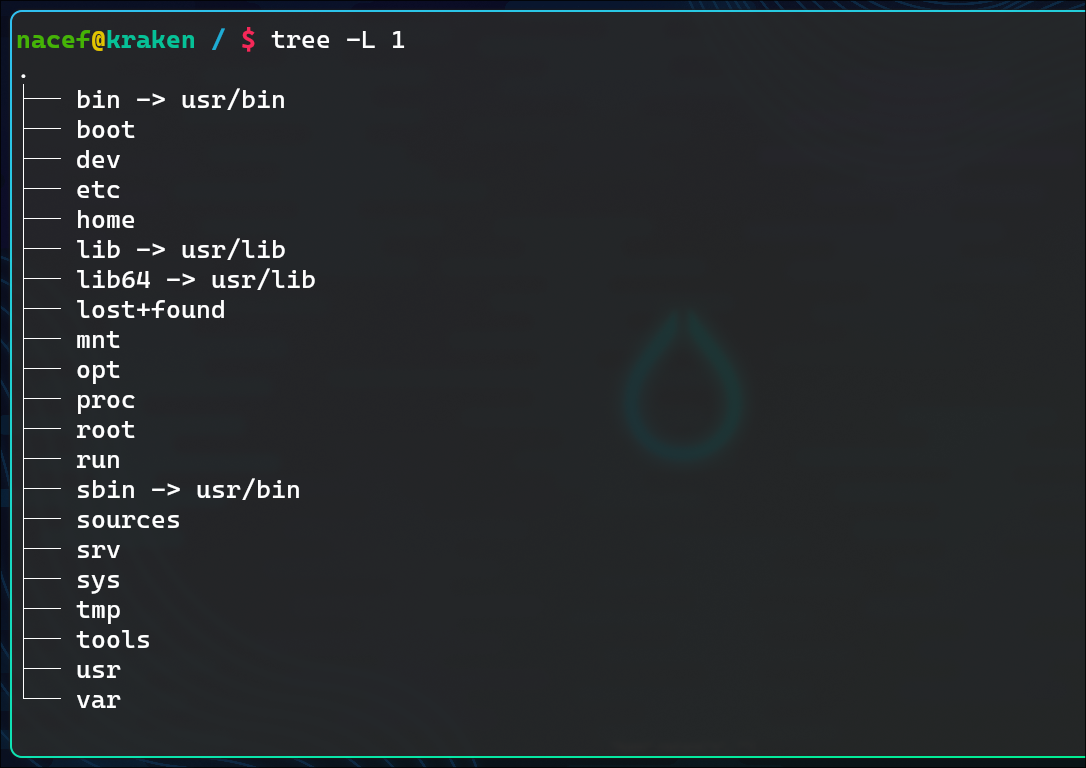
\includegraphics[width=1\textwidth, height=10cm]{images_pfe/minimalfhs.png}
  \caption{Hiérarchie minimale des répertoires conforme au standard FHS}
  \label{fig:minimlfhs}
\end{figure}

\textbf{Remarque :}  
\begin{itemize}
  \item \textbf{Répertoire \texttt{sources}} :  
        Servira à compiler tous les paquets du système.
  \item \textbf{Répertoire \texttt{tools}} :  
        Contiendra le cross-compilateur et sa toolchain.
\end{itemize}

\subsection{Pré-configuration}
Lorsqu’on est connecté en tant que \texttt{root}, une seule erreur peut endommager ou détruire le système. \\Nous devons donc créer un utilisateur dédié et configurer son groupe ainsi que les droits d’accès sur les répertoires et fichiers de l’arborescence. Cet utilisateur sera utilisé pour compiler et configurer les paquets.

\textbf{Outils utilisés}~:  
\texttt{groupadd}, \texttt{useradd}, \texttt{passwd}, \texttt{chown}, \ldots 

Nous devons également ajouter des configurations supplémentaires relatives aux options de compilation et à l’environnement pour préparer le développement de notre compilateur croisé.\\
\clearpage
Exemple de configuration du \texttt{.bashrc} :

\begin{verbatim}
set +h
umask 022
KRAKEN=/mnt/kraken
KRAKEN_TGT=x86-64-kraken-linux-gnu
PATH=$KRAKEN/tools/bin:$PATH

\end{verbatim}

\textbf{Explications~:}

\begin{itemize}
    \item \textbf{set +h:} 
          Désactive l'utilisation de la table de hachage (\emph{hash table}) de Bash. 
          L idee est de \textbf{FORCER} Le shell de rechercherer  les exécutables dans le \texttt{PATH}   plutôt que de mémoriser leurs emplacements.

    \item \textbf{umask 022:} 
          Définit les permissions par défaut pour les nouveaux fichiers/répertoires~: 
         

    \item \textbf{KRAKEN=/mnt/kraken~:} 
          Variable pointant vers le disque monté où notre système sera construit.

    \item \textbf{KRAKEN-TGT=x86-64-kraken-linux-gnu~:} 
          Définit la cible du compilateur croisé. Cette configuration est importante permet de simuler un environnement hôte différent, comme détaillé dans la section suivante.

   

    \item \textbf{/mnt/kraken/tools/bin:PATH~:}
            Permet au shell de détecter immédiatement notre compilateur croisé situé dans \texttt{/tools/bin}.
\end{itemize}

\textcolor{blue}{Pour plus d’informations sur  la préparation de l’environnement hôte  consultez \cite{lfs_book} }









% ----- Compilation croisée -----------
\section{Construction du compilateur croisé et des bibliothèques associées}
\label{subsec:build-cross}
Les etapes principales sont:\\
\begin{enumerate}
  \item Developemnt du compilateur croisé.
  \item Utilisation de ce compilateur pour assembler une chaîne d’outils temporaire.
  \item Emploi de cette chaîne d’outils pour bâtir le système final.
\end{enumerate}

\subsection{Compilateur croisé}
Comme discuté dans le chapitre  \ref{subsec:cross-compiler} sur la compilation, nous devons créer un compilateur croisé «~factice~».  




\subsubsection{Concept clé~: le triplet système}  
Le système de construction basé sur \texttt{autoconf} utilise un format \texttt{cpu-vendor-kernel-os} (appelé «~triplet système~»).

%\textbf{Remarque~:} Si vous vous interrogez sur l’appellation «~triplet~» pour une structure à quatre composants,  voir la section~\hyperref[sec:triplet]{\textcolor{blue}{\ref*{sec:triplet}}} de l'annexe. 

%\subsubsection{Implémentation du compilateur factice}  
Pour simuler le compilateur croisé~:  
\begin{itemize}  
  \item Il faut Modifiez la cible (\texttt{--target}) durant la compilation des paquets~;  
  \item \textbf{Spécifiquement}~: le champ \texttt{vendor}  du triplet système.  
  \begin{itemize}  
    \item Cette approche indique au compilateur d’installer les paquets dans un emplacement différent (\texttt{/mnt/kraken}) plutôt que sur le système hôte.  
  \end{itemize}  
  \item Ajoutez l’option \texttt{--with-sysroot=/mnt/kraken}~:  
  \begin{itemize}  
    \item Force le compilateur à rechercher les bibliothèques \textbf{uniquement} dans notre système (\texttt{/mnt/kraken}),  
    \item Garantit qu’il ne lie \textbf{aucune bibliothèque} du système hôte.  
  \end{itemize}  
\end{itemize}  


Ce compilateur croisé est composé des paquets suivants~:

\begin{table}[H]
    \centering
    \begin{tabular}{|c|p{8cm}|}
        \hline
        \textbf{Paquet}  & \textbf{Fonction principale} \\
        \hline
       GCC                & Compilateur C/C++ (base de la chaîne d’outils) \\
        \hline
        Binutils             & Fournit l’éditeur de liens (\texttt{ld}) et le vérificateur de dépendances (\texttt{ldd}). \\
        \hline
        Linux-API Headers         &   En-têtes du noyau Linux (nécessaires pour la compilation des bibliothèques système). \\
        \hline
        Glibc          & Bibliothèque C GNU (implémente les fonctions de base comme \texttt{printf}, \texttt{malloc}, etc.) etc.) \\
        \hline
        Libstdc++       & Bibliothèque standard C++ (fournit \texttt{std::string}, \texttt{std::vector}, etc.). \\
       
       
        \hline
    \end{tabular}
    \caption{Composants du compilateur croisé}
    \label{tab:crosscompiler}
\end{table}

%\begin{table}[H]
%    \centering
%    \begin{tabular}{|c|c|p{8cm}|}
%        \hline
%        \textbf{Paquet} & \textbf{Version} & \textbf{Fonction principale} \\
%        \hline
%       GCC             & 14.2.0    & Compilateur C/C++ (base de la chaîne d’outils) \\
%        \hline
%        Binutils        & 2.44       & Fournit l’éditeur de liens (\texttt{ld}) et le vérificateur de dépendances (\texttt{ldd}). \\
%        \hline
%        Linux-API Headers         &6.13.4    &   En-têtes du noyau Linux (nécessaires pour la compilation des bibliothèques système). \\
%        \hline
%        Glibc      & 2.41       & Bibliothèque C GNU (implémente les fonctions de base comme \texttt{printf}, \texttt{malloc}, etc.) etc.) \\
 %       \hline
 %       Libstdc++     & 3.10      & Bibliothèque standard C++ (fournit \texttt{std::string}, \texttt{std::vector}, etc.). \\
       
       
 %       \hline
 %   \end{tabular}
 %   \caption{Composants du compilateur croisé}
 %   \label{tab:crosscompiler}
%\end{table}

Ces paquets doivent être configurés avec un préfixe et une cible spécifiques~:
\begin{verbatim}
--prefix=/mnt/kraken/tools
--with-sysroot=/mnt/kraken
--target=x86_64-kraken-linux-gnu
\end{verbatim}

\noindent
Exemple de configuration du paquet \texttt{gcc}~:

\begin{verbatim}
../configure                  \
    --target=$KRAKEN_TGT      \
    --prefix=$KRAKEN/tools    \
    --with-sysroot=$KRAKEN    \     
    --disable-libstdcxx       \
    --enable-languages=c,c++
\end{verbatim}

\textbf{Explications~:}
\begin{itemize}
  \item \textbf{\texttt{--disable/--enable}}~: 
        Active/désactive des fonctionnalités spécifiques durant la compilation.
        
  \item \textbf{\texttt{--target=x86\_64-kraken-linux-gnu} et \texttt{--with-sysroot=/mnt/kraken}}~: 
        Simulent un compilateur croisé en redirigeant :
        \begin{itemize}
          \item La cible vers une architecture personnalisée,
          \item La recherche des bibliothèques vers le système isolé.
        \end{itemize}
        
  \item \textbf{\texttt{--prefix=/mnt/kraken/tools}}~: 
        Définit le répertoire d’installation du compilateur croisé.
\end{itemize}


\subsection{Construction des outils temporaires}
\label{subsec:outils-temp}

Cette section décrit la compilation des utilitaires de base à l’aide de notre nouvelle chaîne d’outils croisée.

Les paquets suivants sont construits en mode cross-compile :
\begin{table}[H]
    \centering
    \begin{tabular}{|c|p{8cm}|}
        \hline
        \textbf{Paquet} & \textbf{Fonction principale} \\
        \hline
        M4               & Traitement des macros dans le code source \\
        \hline
        Ncurses             & Gestion avancée de l’affichage en terminal \\
        \hline
        Bash              & Interpréteur de commandes principal \\
        \hline
        Coreutils             & Commandes système de base (\texttt{ls}, \texttt{cd}, \texttt{mkdir}, etc.) \\
        \hline
        Diffutils            & Comparaison de fichiers et de répertoires \\
        \hline
        File                & Identification du type de fichiers \\
        \hline
        Grep              & Recherche de motifs dans les fichiers \\
        \hline
        Make               & Automatisation des processus de compilation \\
        \hline
        Gettext              & Utilitaires pour l’internationalisation et la localisation \\
        \hline
        Bison              & Générateur d’analyseurs (parser) \\
        \hline
        Perl              & Langage pratique d’extraction et de rapports \\
        \hline
        Python           & Environnement de développement Python \\
        \hline
        Texinfo             & Programmes pour lire, écrire et convertir des pages \texttt{info} \\
        \hline
        Util-linux        & Divers utilitaires système \\
        \hline
    \end{tabular}
    \caption{Chaîne d’outils essentielle}
    \label{tab:toolchain}
\end{table}

%\begin{table}[H]
 %   \centering
 %   \begin{tabular}{|c|c|p{8cm}|}
 %       \hline
 %       \textbf{Paquet} & \textbf{Version} & \textbf{Fonction principale} \\
 %       \hline
 %       M4             & 1.4.19    & Traitement des macros dans le code source \\
 %       \hline
 %       Ncurses        & 6.5       & Gestion avancée de l’affichage en terminal \\
 %       \hline
 %       Bash           & 5.2.32    & Interpréteur de commandes principal \\
 %       \hline
     %   Coreutils      & 9.5       & Commandes système de base (\texttt{ls}, \texttt{cd}, \texttt{mkdir}, etc.) \\
    %    \hline
    %    Diffutils      & 3.10      & Comparaison de fichiers et de répertoires \\
    %    \hline
    %    File           & 5.45      & Identification du type de fichiers \\
    %    \hline
    %    Grep           & 3.11      & Recherche de motifs dans les fichiers \\
    %    \hline
    %    Make           & 4.4.1     & Automatisation des processus de compilation \\
    %    \hline
    %    Gettext        & 0.24      & Utilitaires pour l’internationalisation et la localisation \\
    %    \hline
    %    Bison          & 3.8.2     & Générateur d’analyseurs (parser) \\
    %    \hline
      %  Perl           & 5.40.1    & Langage pratique d’extraction et de rapports \\
      %  \hline
      %  Python         & 3.13.2    & Environnement de développement Python \\
      %  \hline
      %  Texinfo        & 7.2       & Programmes pour lire, écrire et convertir des pages \texttt{info} \\
      %  \hline
      %  Util-linux     & 2.40.4    & Divers utilitaires système \\
      %  \hline
    %\end{tabular}
    %\caption{Chaîne d’outils essentielle}
    %\label{tab:toolchain}
%\end{table}

Exemple dinstallation du paquete M4 :

\begin{verbatim}
    ./configure --prefix=/usr   \
            --host=x86_64-kraken-linux-gnu \
            
        && 
        make
         &&
        make DESTDIR=/mnt/kraken install    
\end{verbatim}


\section{Installation des logiciels système de base}
\label{subsec:install-base}

À ce stade, nous disposons d’une chaîne d’outils complète et pouvons commencer la construction effective de \textsc{Kraken OS}. Les paquets compilés ici sont les versions finales du système. Avant leur installation, il est nécessaire de se placer dans l’environnement chroot correspondant.




\subsection{Chroot vers le nouveau système}
\label{sssec:chroot}

À ce stade, Nous créons un environnement \texttt{chroot} totalement isolé du système hôte (à l’exception du noyau en cours d’exécution). Pour que cet environnement isolé fonctionne correctement, nous devons monter les systèmes de fichiers virtuels du noyau avant d’y entrer.

\paragraph{Préparation des systèmes de fichiers virtuels}
Dans l’arborescence de montage, nous créons les répertoires suivants :
\begin{verbatim}
/dev
/proc
/sys
/run
\end{verbatim}

\textbf{Explications~:}
\begin{itemize}
  \item \texttt{/proc}~: Interface de communication avec le noyau (processus, paramètres système).
  \item \texttt{/dev}~: Points d’accès aux périphériques matériels.
  \item \texttt{/sys}~: Informations sur le matériel et les pilotes en temps réel.
  \item \texttt{/run}~: Données temporaires volatiles .\\
\end{itemize}
Puis nous montons les systèmes de fichiers du noyau hôte :\\

\begin{verbatim}
mount -vt devpts devpts -o gid=5,mode=0620 /mnt/kraken/dev/pts
mount -vt proc   proc   /mnt/kraken/proc
mount -vt sysfs  sysfs  /mnt/kraken/sys
mount -vt tmpfs  tmpfs  /mnt/kraken/run
\end{verbatim}

\textbf{Explications des montages~:}
\begin{itemize}
  \item \texttt{devpts}~: 
        Système de fichiers des pseudo-terminaux esclaves, essentiel pour les commandes nécessitant un terminal (ex: \texttt{sudo}).
        
  \item \texttt{sysfs}~: 
        Expose les informations matérielles et des pilotes à l’espace utilisateur.
        
  \item \texttt{tmpfs}~: 
        Système de fichiers temporaire en RAM pour les données d’exécution volatiles.
        
  \item \texttt{gid=5, mode=0620}~: 
        \begin{itemize}
          \item \texttt{gid=5}~: Associe le groupe \texttt{tty} (id=5) aux pseudo-terminaux,
          \item \texttt{mode=0620}~: Définit les permissions .
        \end{itemize}
\end{itemize}
\noindent
Une fois ces montages effectués, nous pouvons entrer dans le chroot :

\begin{verbatim}
chroot "/mnt/kraken" /usr/bin/env -i \
  HOME=/root                  \
  PATH=/usr/bin:/usr/sbin     \
  MAKEFLAGS="-j6"      \
  /bin/bash --login
\end{verbatim}
\textbf{Explications des configurations importantes :}
\begin{itemize}
  \item \texttt{chroot "/mnt/kraken" /usr/bin/env -i} :  
        Isole l’environnement en réinitialisant les variables système .



  \item \texttt{MAKEFLAGS="-j6"} :  
        Utilise six cœurs du processeur  pour accélérer la compilation.

  \item \texttt{/bin/bash --login} :  
        Force une session de connexion complète au premier accès du \texttt{chroot}.
\end{itemize}

Avant de débuter l’installation, nous modifions plusieurs configurations critiques dans l’environnement chroot :

\begin{itemize}
  \item \textbf{Création des sous‑répertoires critiques}, par exemple :
    \begin{itemize}
      \item \texttt{/lib/firmware}           : stockage des chargeurs d’amorçage  
      \item \texttt{/etc/sysconfig}          : configurations système  
      \item \texttt{/media/floppy, cdrom}    : points de montage pour supports amovibles  
      \item \texttt{/usr/{,local/}share/\{color,dict,doc,info,locale,man\}} : documentation et données partagées  
      \item \texttt{/var/\{cache,local,log,mail,opt,spool\}}             : fichiers variables  
    \end{itemize}

  \item \textbf{Création de liens symboliques essentiels} :
    \begin{itemize}
      \item \texttt{/proc/self/mounts} → \texttt{/etc/mtab}  
      \item \texttt{/var/run}           → \texttt{/run}  
    \end{itemize}
\end{itemize}









\subsection{Compilation et installation des paquets système finaux avec notre chaîne d’outils}
\label{sssec:install-final}

Nous entrons maintenant dans la phase finale de construction, avec l’installation des 80 paquets fondamentaux :
\begin{table}[H]
\centering
\begin{tabular}{|l|l|}
\hline
\textbf{Catégorie} & \textbf{Exemples de paquets} \\
\hline
Noyau et bas niveau & Glibc, Binutils, GCC \\
\hline
Compression et archivage & Zlib, Xz \\
\hline
Outils de compilation & Make, Autoconf, Meson, Flex \\
\hline
Langages et développement & Python, Perl \\
\hline
Shell et interface utilisateur & Bash, Ncurses, Readline \\
\hline
Utilitaires Unix essentiels & Coreutils, Gawk, Grep \\
\hline
Réseau & IPRoute2, Inetutils \\
\hline
Système de fichiers & Util-linux, Udev \\
\hline
Gestion du système & SysVinit \\
\hline
Documentation & Man-pages, Texinfo \\
\hline
Gestion de paquets & Pkgconf \\
\hline
Chargeur de démarrage & GRUB \\
\hline
\end{tabular}
\caption{Catégories des paquets système finaux}
\label{tab:categories-paquets}
\end{table}



%\begin{itemize}
%    \item \textbf{Noyau et bas niveau} : Glibc-2.40, Binutils-2.43.1, GCC-14.2.0  
%    \item \textbf{Gestion de paquets} : Pkgconf-2.3.0, Dpkg-1.22.6  
%    \item \textbf{Sécurité} : Libcap-2.70, Shadow-4.16.0  
%    \item \textbf{Réseau} : IPRoute2-6.10.0, OpenSSL-3.3.1  
%    \item \textbf{Interface utilisateur} : Ncurses-6.5, Bash-5.2.32  
%\end{itemize}

%Liste complète des paquets critiques :

%\begin{verbatim}
%Man-pages-6.9.1        Iana-Etc-20240806     Glibc-2.40
%Zlib-1.3.1             Bzip2-1.0.8           Xz-5.6.2
%Lz4-1.10.0             Zstd-1.5.6            File-5.45
%Readline-8.2.13        M4-1.4.19             Bc-6.7.6
%Flex-2.6.4             Tcl-8.6.14            Expect-5.45.4
%DejaGNU-1.6.3          Pkgconf-2.3.0         Binutils-2.43.1
%GMP-6.3.0              MPFR-4.2.1            MPC-1.3.1
%Attr-2.5.2             Acl-2.3.2             Libcap-2.70
%Libxcrypt-4.4.36       Shadow-4.16.0         GCC-14.2.0
%Ncurses-6.5            Sed-4.9               Psmisc-23.7
%Gettext-0.22.5         Bison-3.8.2           Grep-3.11
%Bash-5.2.32            Libtool-2.4.7         GDBM-1.24
%Gperf-3.1              Expat-2.6.2           Inetutils-2.5
%Less-661               Perl-5.40.0           XML::Parser-2.47
%Intltool-0.51.0        Autoconf-2.72         Automake-1.17
%OpenSSL-3.3.1          Kmod-33               Libelf (Elfutils-0.191)
%Libffi-3.4.6           Python-3.12.5         Flit-Core-3.9.0
%Wheel-0.44.0           Setuptools-72.2.0     Ninja-1.12.1
%Meson-1.5.1            Coreutils-9.5         Check-0.15.2
%Diffutils-3.10         Gawk-5.3.0            Findutils-4.10.0
%Groff-1.23.0           GRUB-2.12             Gzip-1.13
%IPRoute2-6.10.0        Kbd-2.6.4             Libpipeline-1.5.7
%Make-4.4.1             Patch-2.7.6           Tar-1.35
%Texinfo-7.1            Vim-9.1.0660          MarkupSafe-2.1.5
%Jinja2-3.1.4           Udev                  Man-DB-2.12.1
%Procps-ng-4.0.4        Util-linux-2.40.2     E2fsprogs-1.47.1
%Sysklogd-2.6.1         SysVinit-3.10
%\end{verbatim}


Exemple dinstallation du paquete Flex :

\begin{verbatim}
    ./configure --prefix=/usr \                #Configuration 
            --docdir=/usr/share/doc/flex-2.6.4 \
            
     && 
        make  #Compilation
     &&
        make check   #Test
     &&
         make install  #Installation
     &&
         ln -sv flex   /usr/bin/lex   #Liens symboliques
     &&
         ln -sv flex.1 /usr/share/man/man1/lex.1  #Documentation
\end{verbatim}

\textbf{Remarque :} Ce chapitre est principalement inspiré du livre LFS, que ce soit pour le compilateur croisé, le choix des paquets, leurs versions ou certaines configurations.

\textcolor{blue}{Pour plus d’informations, voir~: \cite{lfs_book}}
 
\section{Conclusion}
À ce stade, nous disposons d’un système minimal fonctionnel. Dans la section suivante, nous verrons la configuration du chargeur d’amorçage, la rédaction des scripts de démarrage et l’intégration du noyau pour rendre le système amorçable.```
\clearpage
% kernel and make the system bootable 

\chapter{ Configuration du noyau et amorçage du système et systemV}
\minitoc
\clearpage

\label{sec:kernel-boot}
\section{Introduction}
Démarrer un système Linux implique plusieurs tâches :  
le processus doit monter les systèmes de fichiers virtuels et réels, initialiser les périphériques, vérifier l’intégrité des systèmes de fichiers, monter et activer les partitions ou fichiers d’échange (swap), régler l’horloge système, mettre en service le réseau, démarrer les démons requis et accomplir toute autre tâche personnalisée spécifiée par l’utilisateur.  

\medskip  
Ce processus doit être organisé pour garantir l’exécution des tâches dans le bon ordre et assurer une rapidité optimale.

\section{Configuration des scripts System V}
\label{sssec:sysv-scripts}

System V est le processus d’amorçage classique sous Linux (cf. chapitre \textcolor{blue}{\ref{sssec:sysv}}). Les scripts suivants sont installés dans \texttt{/etc/rc.d} avec un lien symbolique dans \texttt{/etc/init.d}:



\begin{table}[H]
  \centering
  \caption{Exemple Scripts System V et leurs descriptions}
  \label{tab:sysv-scripts}
  \begin{tabularx}{\linewidth}{|l|X|}
    \toprule
    \textbf{Script} & \textbf{Description} \\
    \midrule
    checkfs      & Vérifie l’intégrité des systèmes de fichiers avant leur montage . \\ \hline
    cleanfs      & Supprime les fichiers temporaires entre redémarrages (\texttt{/run}, \texttt{/var/lock}) . \\ \hline
    console      & Charge la table de clavier appropriée et définit la police d’écran. \\ \hline
    halt         & Arrête et éteint le système. \\ \hline
    ifdown       & Désactive une interface réseau. \\ \hline
    ifup         & Active et configure une interface réseau.  \\ \hline
    mountfs      & Monte tous les systèmes de fichiers . \\ \hline
    mountvirtfs  & Monte les systèmes de fichiers virtuels du noyau (\texttt{proc}, \texttt{sysfs}, \texttt{devpts}, \texttt{run}). \\ \hline
    reboot       & Redémarre le système. \\ \hline
    setclock     & Réinitialise l’horloge système à l’heure locale . \\ \hline
    swap         & Active et désactive les partitions ou fichiers d’échange (\texttt{swap}). \\ \hline
     
    \bottomrule
  \end{tabularx}
\end{table}

Tous ces scripts suivent le même modèle : une structure basée sur une simple  `case statement` qui gère les arguments `start`|`stop`|`restart`.  

\begin{figure}[H]  
  \centering  
  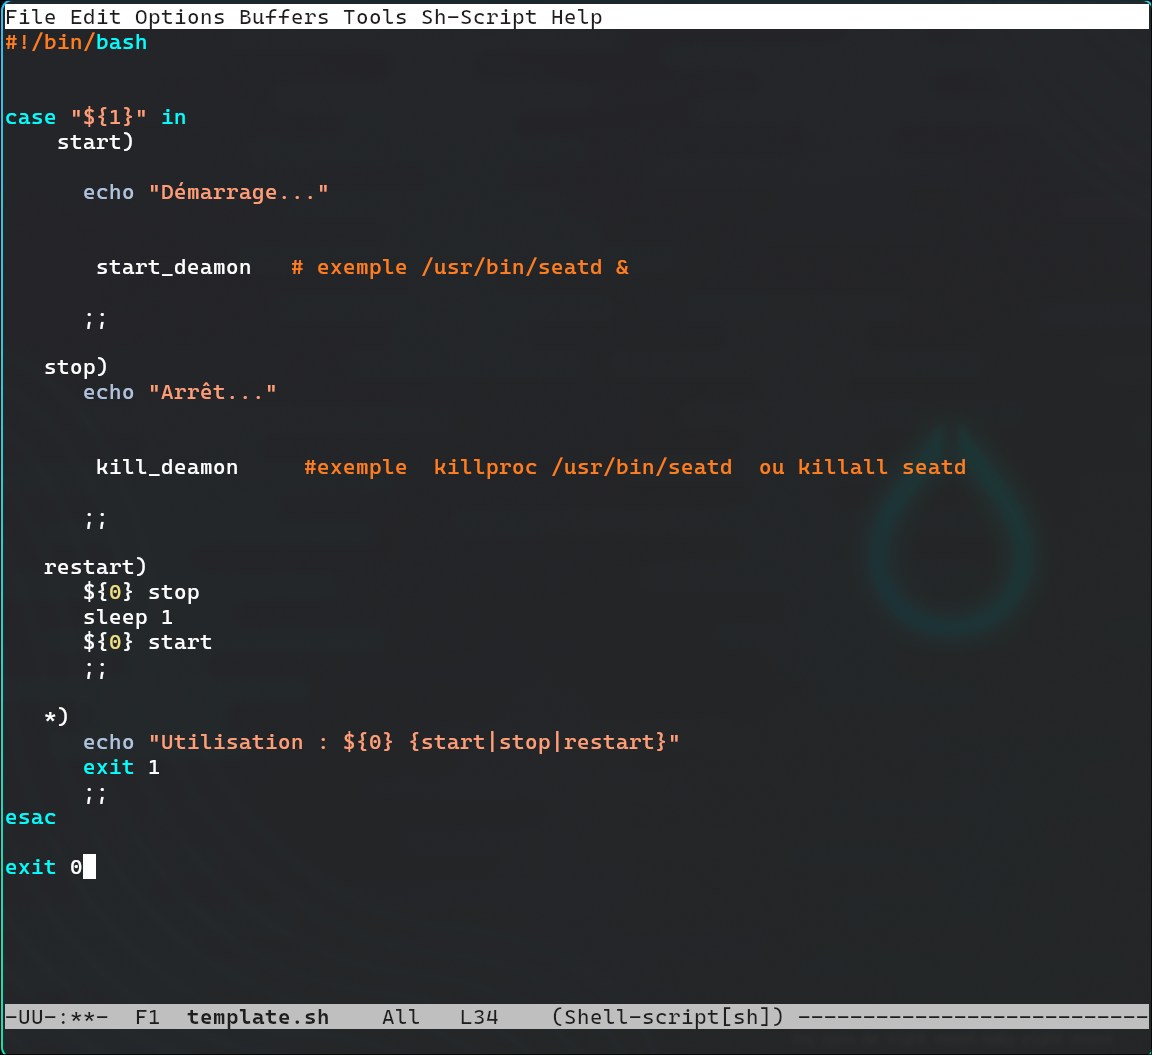
\includegraphics[width=1\textwidth]{images_pfe/systemvtemplate.png}  
  \caption{Exemple de template d’un script de démarrage} 
  \label{fig:systemvtemplate}  
\end{figure}  
\textbf{Remarque} : Nous utilisons les scripts de démarrage de BLFS, que nous avons enrichis avec d'autres simple scripts.  
\textcolor{blue}{Pour plus d'informations sur les scripts BLFS, consultez \cite{blfs_bootscripts}.}

%\subsection{Configurations importantes}
%\label{subsec:config-importantes}

%La configuration du système requiert plusieurs fichiers critiques à ajuster :

%\begin{itemize}
 % \item \textbf{Configuration de l’horloge système} — %\texttt{/etc/sysconfig/clock}  
 % Ce fichier définit le comportement de l’horloge (UTC ou heure locale).
 % simplement ellecentien 
 % \begin{verbatim}
 %     UTC=1 #mean set hardware clock  to UTC (Coordinated Universal Time).
 % \end{verbatim}

  %\item \textbf{Configuration de la console Linux} — %\texttt{/etc/sysconfig/console}  
  %Permet de spécifier la table de caractères, la police et la disposition du %clavier.
  % \begin{verbatim}
  %    LOGLEVEL="3"  # Kernel log verbosity level
  %    UNICODE="1"  # Enable Unicode support
  %    FONT="Lat2-Terminus16". # Console font to use
      
  %\end{verbatim}

  %\item \textbf{Configuration de la locale système} et création de %\texttt{/etc/profile}  
  %Le fichier \texttt{/etc/locale.conf} définit la langue et le jeu de %caractères par défaut 

 

  %\item \textbf{Liste des shells valides} — \texttt{/etc/shells}  
  %Contient les chemins des interpréteurs de commandes autorisés pour les %utilisateurs.

  

  %\item \textbf{Configuration réseau} — %\texttt{/etc/sysconfig/ifconfig.enp0s3}, , \texttt{/etc/hosts}  
  %Ces fichiers déterminent l’adresse IP statique, les serveurs DNS et la %résolution locale des noms d’hôtes.

  
%\end{itemize}

\section{Compilation et paramétrage du noyau Linux}
\label{subsec:compilation-noyau}

Notre implémentation s’appuie sur le noyau version \texttt{6.5.10}, retenu pour son support matériel étendu et ses correctifs de sécurité récents. Nous devons configurer, compiler puis installer ce noyau.

Le noyau Linux comporte environ 12 000 options de configuration. Il est essentiel de sélectionner précisément celles dont nous avons besoin pour optimiser la taille, la sécurité et les performances.
\clearpage
La configuration du noyau Linux s'effectue généralement via l'interface menuconfig, accessible grâce à la commande :\\
\begin{verbatim}
   make menuconfig
\end{verbatim}

\begin{figure}[H]
  \centering
  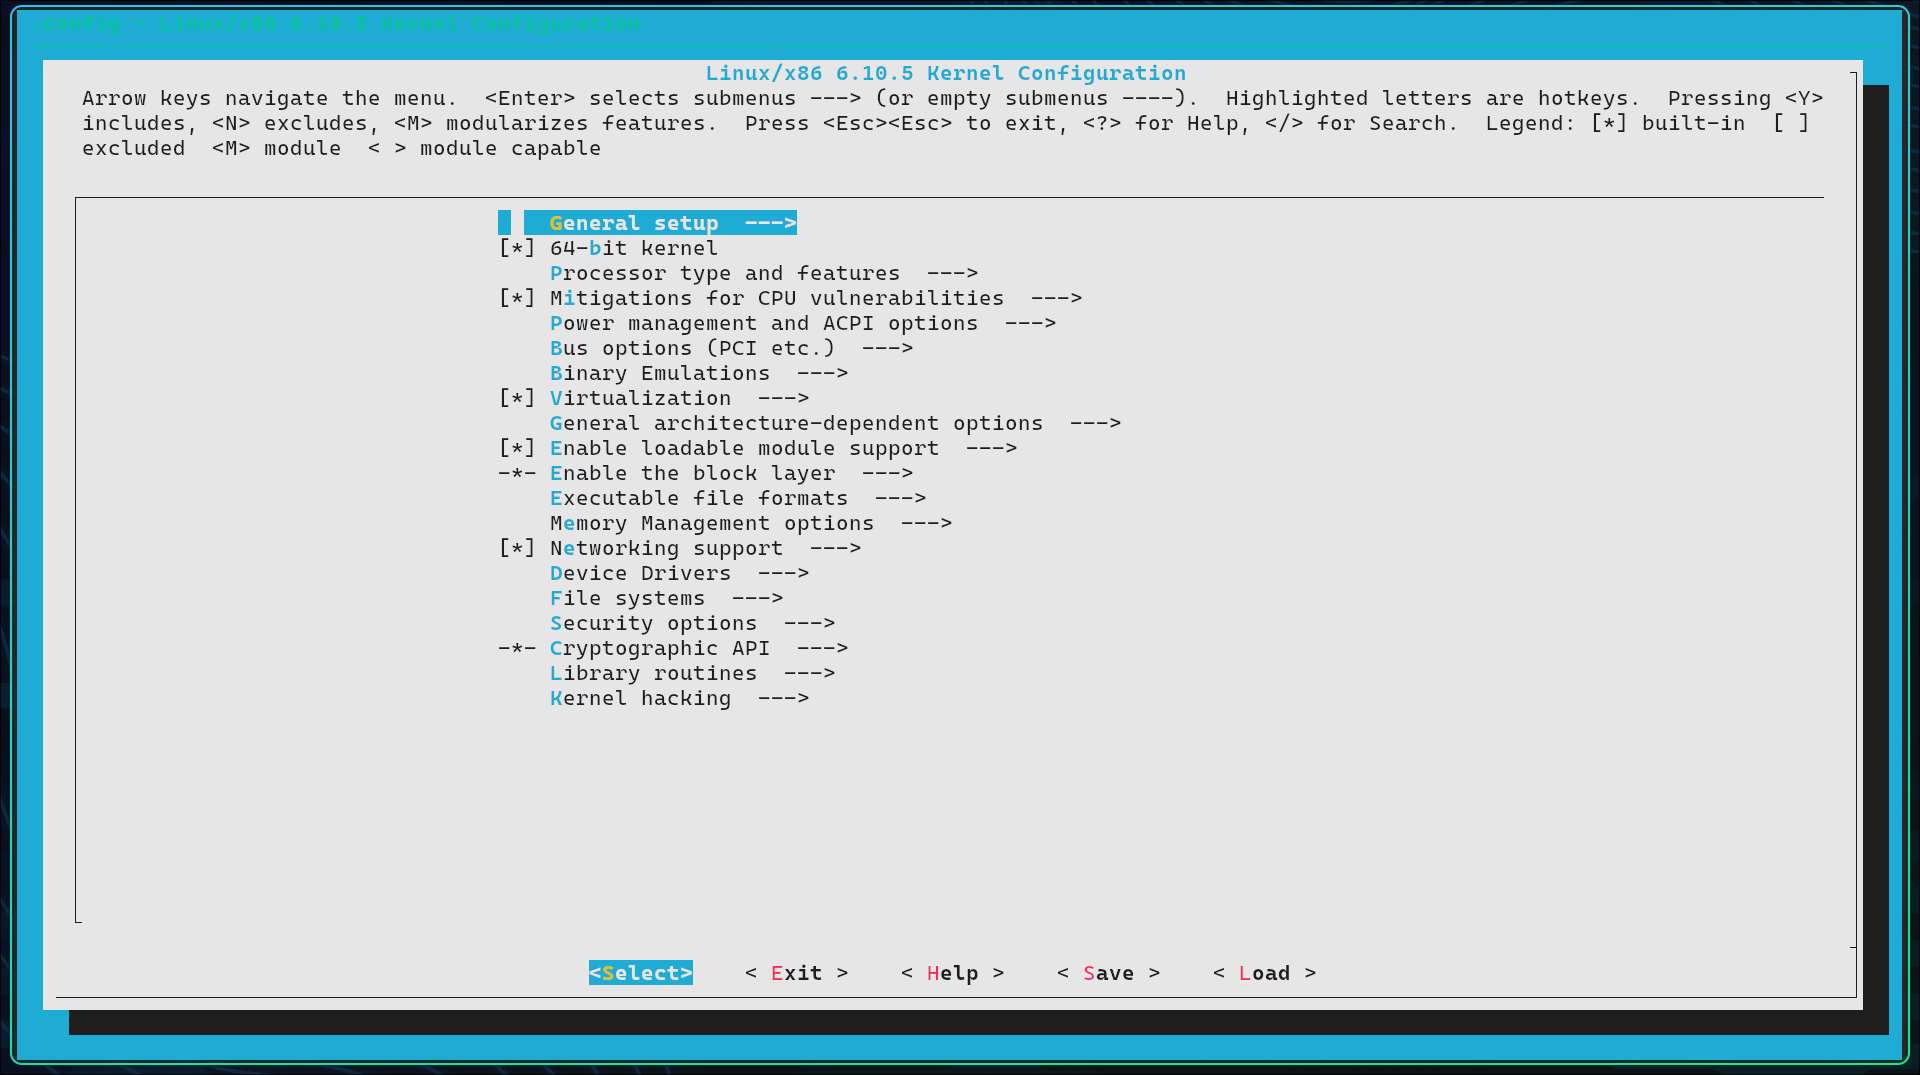
\includegraphics[width=1\textwidth]{images_pfe/kernelmenuconfig.png}
  \caption{Configuration de noyau linux}
  \label{fig:configuration de noyau}
\end{figure}
Nous avons activé environ 1 695 paramètres de configuration.

\textbf{Remarque} : nous n'avons pas configuré manuellement les 1 695 options. Lors de la première étape, nous nous sommes appuyés sur la commande \textbf{make defconfig}, qui génère une configuration de base adaptée à notre architecture \textbf{x86\_64}. 

Ensuite, à l'étape 2, nous avons utilisé \texttt{make menuconfig} pour activer manuellement d'autres options supplémentaires, soit en tant qu’intégrées (\texttt{<*>}), soit en tant que modules (\texttt{<m>}).

Voici un exemple de ces paramètres activés :

\begin{figure}[H]  
  \centering  
  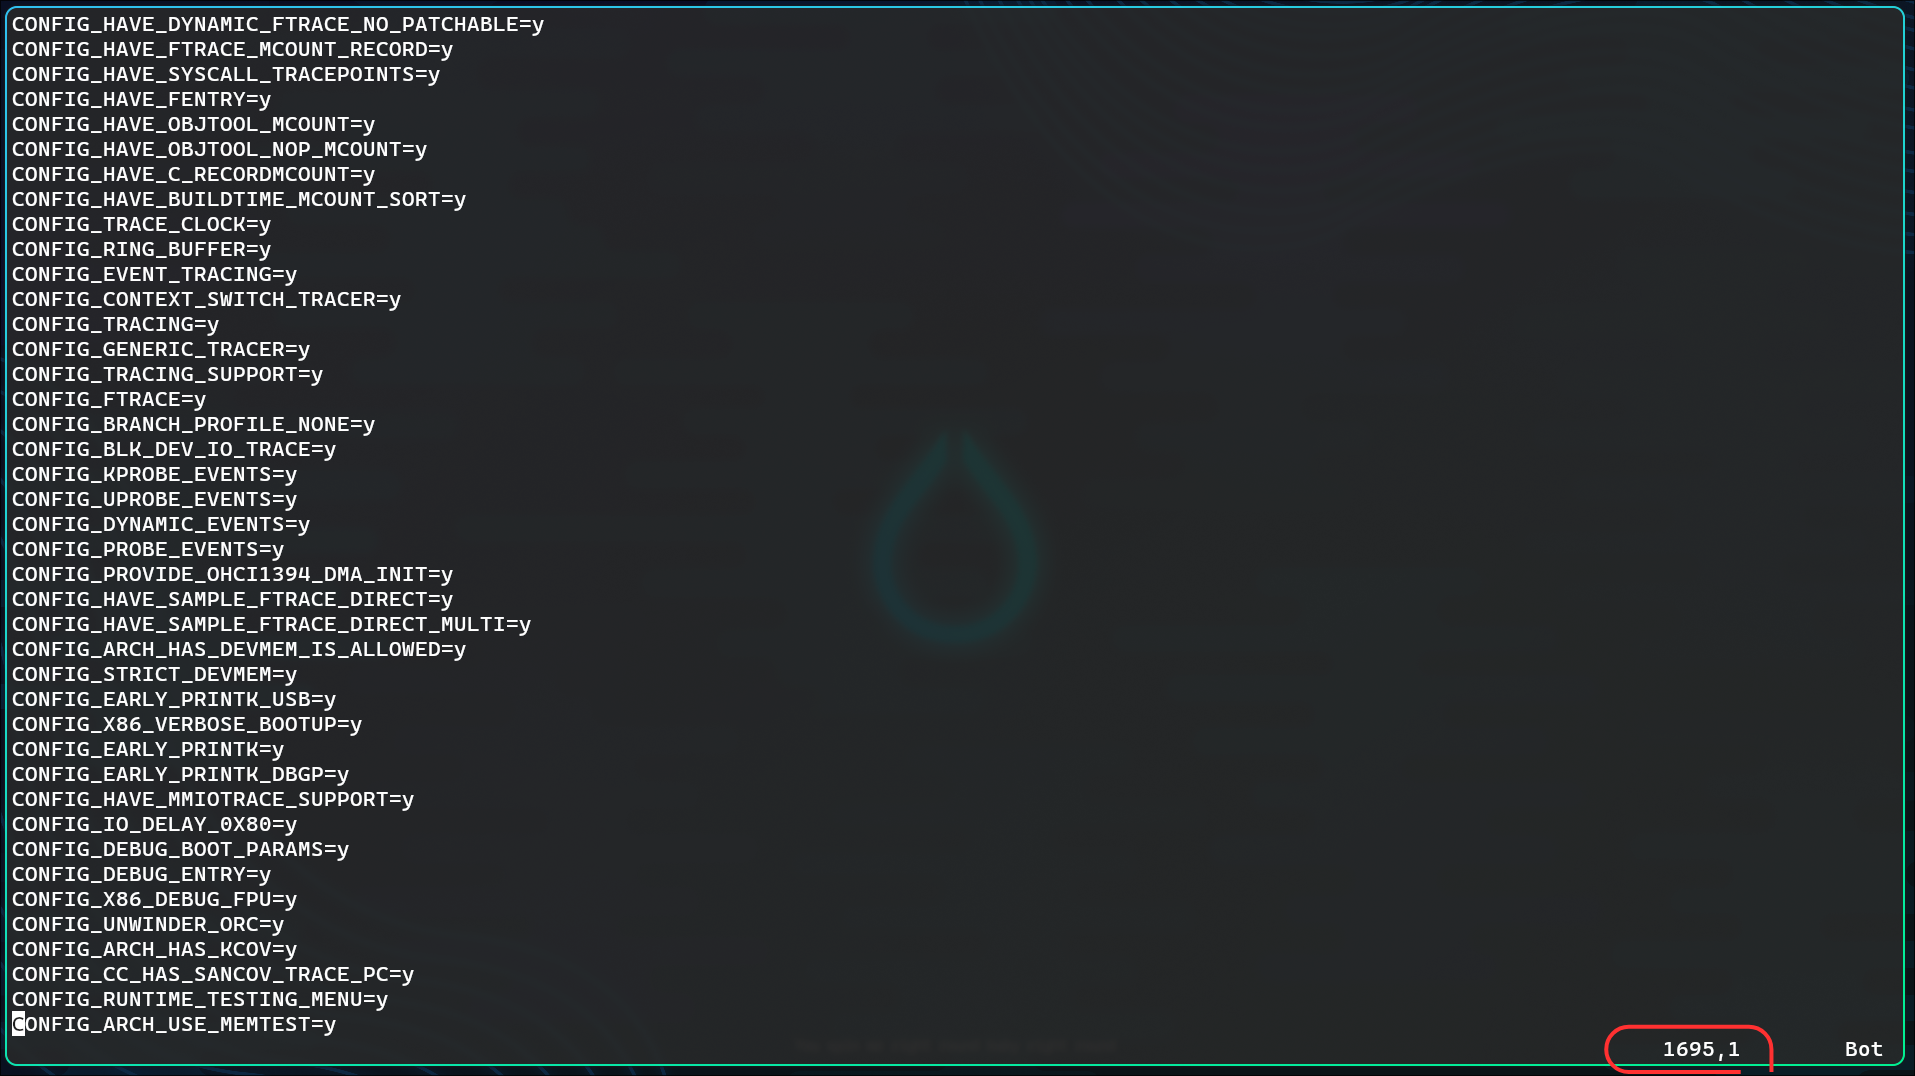
\includegraphics[width=1\textwidth]{images_pfe/numberconfig.png}  
  \caption{Aperçu des paramètres de configuration activés dans \texttt{/boot/config}}  
  \label{fig:kernel_config}  
\end{figure}  



\clearpage
\paragraph*{Fichiers critiques après installation}
\begin{itemize}
  \item \texttt{arch/x86/boot/bzImage} — image binaire du noyau   
  \item \texttt{.config} — fichier de configuration contenant toutes les options sélectionnées  
\end{itemize}

\textit{Remarque :} ces fichiers doivent être configure dans \texttt{/boot} pour être détectés par le chargeur d’amorçage (GRUB) :

\begin{verbatim}
 if faut copier:
 arch/x86/boot/bzImage  dans /boot/vmlinuz-kraken
 config              dans /boot/config
\end{verbatim}


\textcolor{blue}{Pour plus d’informations sur la configuration et la compilation de noyau, consultez \cite{linuxkernel}}
\section{Configuration du processus de démarrage}
\label{sssec:boot}

Le processus de démarrage s’appuie sur deux fichiers principaux : \texttt{/etc/fstab}, qui définit comment et où les périphériques de stockage  sont montés dans la structure de répertoires du système au démarrage, et le fichier de configuration de GRUB \texttt{grub.cfg}.


\begin{enumerate}

  \item \textbf{Exemple de Fichier \texttt{/etc/fstab}}  
  
  \begin{verbatim}


# système de fichiers | point de montage| type | options | dump |fsck-order
#monter les partitions du disque
/dev/sda4      /              ext4     defaults            1     1
/dev/sda3      swap           swap     pri=1               0     0
/dev/sda1      /boot/efi      vfat     codepage=437        0     1
/dev/sda5      /home          ext4     defaults            1     2

#monter les systèmes de fichiers virtuels
proc           /proc          proc     nosuid,noexec,nodev 0     0
sysfs          /sys           sysfs    nosuid,noexec,nodev 0     0
devpts         /dev/pts       devpts   gid=5,mode=620      0     0
tmpfs          /run           tmpfs    defaults            0     0
devtmpfs       /dev           devtmpfs mode=0755,nosuid    0     0
tmpfs          /dev/shm       tmpfs    nosuid,nodev        0     0



  \end{verbatim}
 \textbf{Explications :}
  \begin{itemize}
    \item \textbf{Les quatre premières lignes} servent à monter les partitions du disque dur et activer la swap.
    \item \textbf{Les sept autres lignes} permettent de monter les systèmes de fichiers virtuels.
    \item \textbf{Options :}
    \begin{itemize}
      \item \textbf{dump :} Détermine si une sauvegarde du système de fichiers doit être effectuée (1 = activé, 0 = désactivé). Généralement activé pour les partitions critiques.
      \item \textbf{fsck-order :} Priorité de vérification du système de fichiers au démarrage (0 = aucune, 1 = première priorité, 2 = seconde).\\
    \end{itemize}
  \end{itemize}


  \item \textbf{ Exemple Fichier de configuration de GRUB}  

  \begin{verbatim}

set default=0
set timeout=10
insmod ext2
set root=(hd0,4) 

menuentry "KRAKEN-OS (mode normal)" {
    linux /boot/vmlinuz_kraken root=/dev/sda4 ro
}

menuentry "KRAKEN-OS (mode debug)" {
    linux /boot/vmlinuz_kraken root=/dev/sda4 debug ro
}

menuentry "KRAKEN-OS (mode RAM)" {
    linux /boot/vmlinuz_kraken root=/dev/sda4 ram ro
}

  \end{verbatim}
\end{enumerate}
\textbf{Explications :}
  \begin{itemize}
    \item \textbf{default :} Entrée de menu sélectionnée par défaut (0 = première entrée).
    \item \textbf{timeout :} Délai avant le démarrage automatique (10 secondes).
    \item \textbf{insmod :} Charge un module GRUB nécessaire (ici, le support ext2).
    \item \textbf{menuentry :} Définit une entrée de menu avec des paramètres de démarrage spécifiques.
  \end{itemize}


\clearpage
À ce stade, nous pouvons démarrer le système minimal et visualiser le processus de démarrage.

\begin{figure}[H]
    \centering
    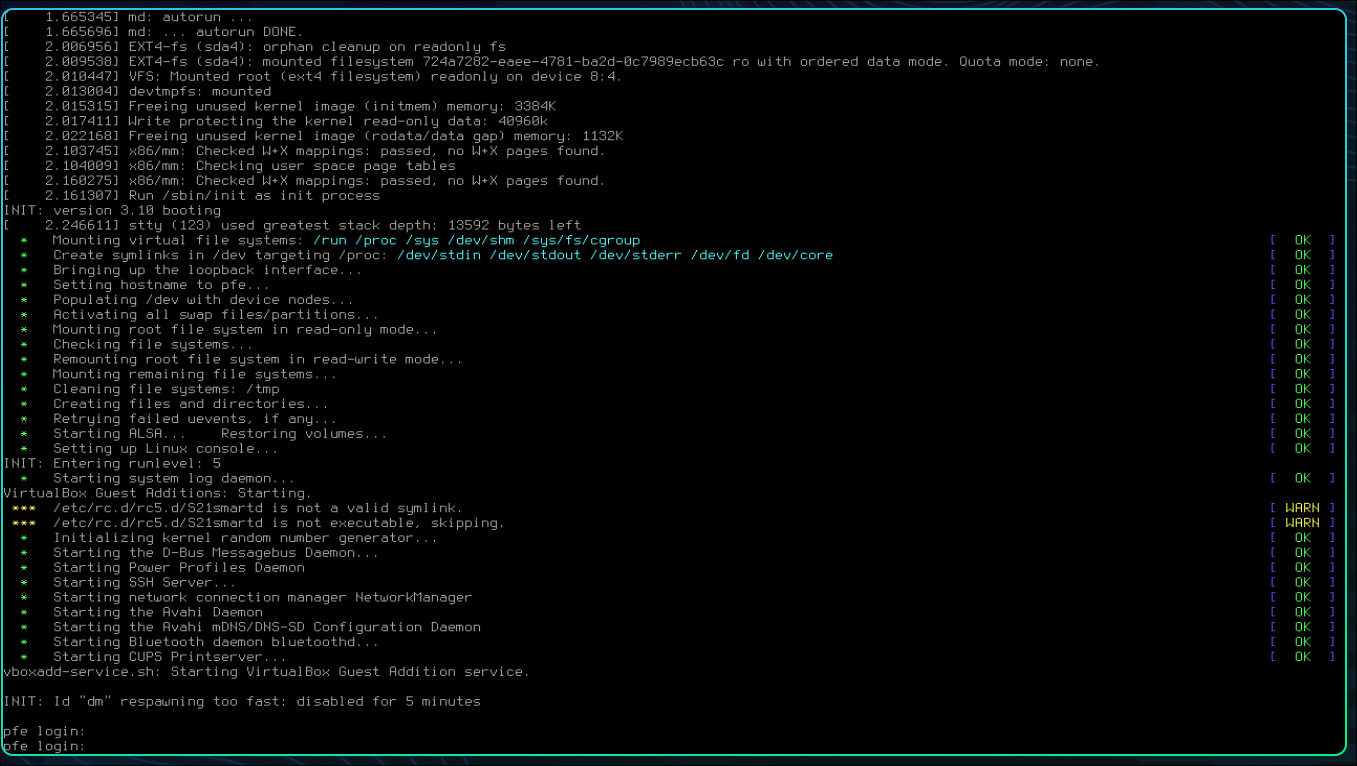
\includegraphics[width=1\textwidth]{images_pfe/corebuildbooscrpts.png}
    \caption{Processus de démarrage}
    \label{fig:bootproc}
\end{figure}

\begin{figure}[H]
    \centering
    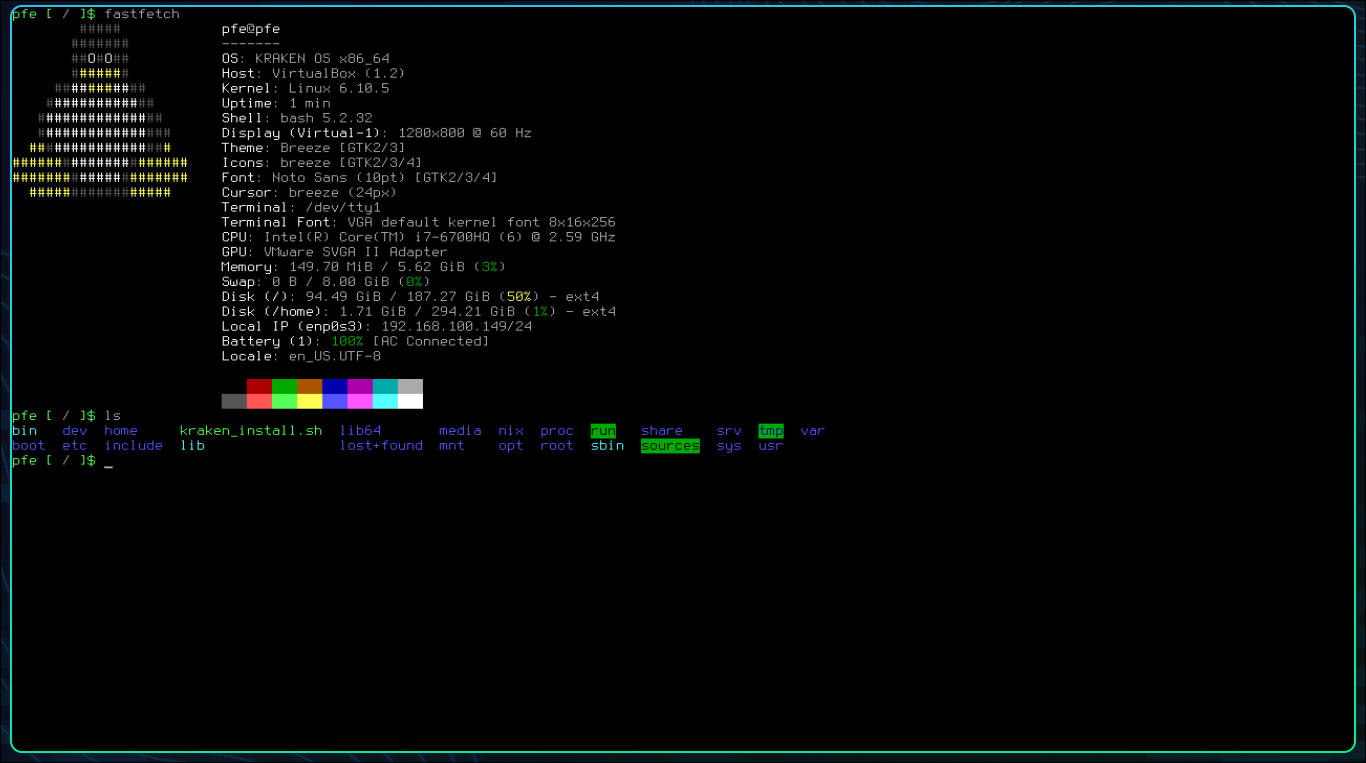
\includegraphics[width=1\textwidth]{images_pfe/corebuildresult.png}
    \caption{Interface TTY du système minimal \textsc{Kraken OS}}
    \label{fig:tty}
\end{figure}

\section{Conclustion}
À ce stade, nous disposons d’une distribution Linux minimale et fonctionnelle, capable de démarrer et d’exécuter des commandes de base.\\
Dans le prochain chapitre, nous passerons à l’étape cruciale : transformer cette base en un système complet et polyvalent.

%----------extends build------------ 
\chapter{  Extendbuild : Ajout des composants avancés}
\minitoc
\clearpage

\section{Introduction}
L’enrichissement du système minimal s’articule autour de deux axes :

\begin{itemize}
 
  \item Installation d’outils et de paquets complémentaires (sécurité, gestion de fichiers et de disques, éditeurs de texte, réseau, etc.).
  \item Configuration de l’environnement graphique ;  
\end{itemize}

\section{Sécurité}
La sécurité se décline en trois volets : l’accès, la prévention et la détection.

\begin{enumerate}
  \item \textbf{Accès} : gestion des sessions utilisateur via l’authentification (login) et renforcement des politiques d’accès à l’aide de modules PAM. Protection de l’accès réseau par des règles iptables (pare‑feu).
  \item \textbf{Prévention} : lutte contre les maliciels (trojans) et chiffrement des données, notamment avec GnuPG.
  \item \textbf{Détection} : surveillance des altérations de fichiers critiques grâce à des outils enregistrant des « empreintes » (hashes).
\end{enumerate}

Exemple des Outils de sécurité installés:
\begin{table}[H]
    \centering
    \begin{tabular}{|c|p{8cm}|}
        \hline
        \textbf{Paquet}  & \textbf{Fonction principale} \\
        \hline
       
        CrackLib  & Vérification de la robustesse des mots de passe contre les attaques par dictionnaire. \\
        \hline
        iptables  & Configuration du pare-feu natif du noyau Linux via des règles de filtrage. \\
        \hline
        GnuPG  & Chiffrement/déchiffrement de données et signatures numériques (implémentation OpenPGP). \\
        \hline
        Sudo  & Délégation sécurisée de commandes privilégiées aux utilisateurs autorisés. \\
        \hline
        Linux-PAM & Framework modulaire pour l'authentification système (login, mot de passe, etc.). \\
        \hline
        OpenSSH  & Suite d'outils de connexion sécurisée à distance . \\
        \hline
        Polkit  & Contrôle granulaire des privilèges pour les processus non-root. \\
        \hline
        Shadow  & Gestion sécurisée des comptes utilisateurs et des mots de passe chiffrés. \\
        \hline
    \end{tabular}
    \caption{Paquets critiques pour la sécurité système}
    \label{tab:security_packages}
\end{table}
 
%\begin{table}[H]
%    \centering
%    \begin{tabular}{|c|c|p{8cm}|}
%        \hline
%        \textbf{Paquet} & \textbf{Version} & \textbf{Fonction principale} \\
%        \hline
%        make-ca & 1.14 & Gestion des certificats racines TLS et mise à jour des magasins de confiance système. \\
 %       \hline
 %       CrackLib & 2.10.2 & Vérification de la robustesse des mots de passe contre les attaques par dictionnaire. \\
 %       \hline
 %       iptables & 1.8.10 & Configuration du pare-feu natif du noyau Linux via des règles de filtrage. \\
 %       \hline
 %       GnuPG & 2.4.5 & Chiffrement/déchiffrement de données et signatures numériques (implémentation OpenPGP). \\
 %       \hline
 %       Sudo & 1.9.15p5 & Délégation sécurisée de commandes privilégiées aux utilisateurs autorisés. \\
%        \hline
 %       Linux-PAM & 1.6.1 & Framework modulaire pour l'authentification système (login, mot de passe, etc.). \\
  %      \hline
   %     OpenSSH & 9.8p1 & Suite d'outils de connexion sécurisée à distance (SSH, SCP, SFTP). \\
   %     \hline
   %     Polkit & 125 & Contrôle granulaire des privilèges pour les processus non-root. \\
   %     \hline
   %     Shadow & 4.16.0 & Gestion sécurisée des comptes utilisateurs et des mots de passe chiffrés. \\
   %     \hline
   % \end{tabular}
   % \caption{Paquets critiques pour la sécurité système}
   % \label{tab:security_packages}
%\end{table}
                   

%\textbf{Exemple d'installation du paquet polkit-125} : outil pour définir et gérer les autorisations.  
%Il permet à des processus non privilégiés de communiquer avec des processus privilégiés.

%\textbf{Dépendances de polkit} :
%\begin{verbatim}
%GLib-2.80.4      duktape-2.7.0       libxslt-1.1.42       Linux-PAM-1.6.1
%elogind-255.5    GTK-Doc-1.34.0      dbusmock-0.32.1 
%docbook-xml-4.5  docbook-xsl-nons-1.79.2
%\end{verbatim}

%\textbf{Configuration requise du noyau} : 
%\begin{verbatim}
%[NAMESPACES], [USER_NS], [AUDIT] (pour l'authentification PAM),  
%[INOTIFY_USER], [TMPFS_POSIX_ACL], [TMPFS], [CRYPTO], [CRYPTO_USER] (pour elogind).
    
%\end{verbatim}

%\textbf{Exemple de compilation de polkit depuis les sources} :
%\begin{verbatim}
%1: Résoudre toutes les dépendances listées ci-dessus
%2: Télécharger l'archive
 %  wget https://github.com/polkit-org/polkit/archive/125/polkit-125.tar.gz
%3: Vérifier l'intégrité de l'archive
 %  md5sum polkit-125.tar.gz  # Doit être 8e9f2377fc7b4010bd29b97d2e288b4f
%4: Extraire l'archive
 %  tar -xvf polkit-125.tar.gz
%5: Accéder au répertoire
%   cd polkit-125
%6: Créer un répertoire de compilation
%   mkdir build && cd build
%7: Configurer (système de build : Meson avec Ninja)
%   meson setup .. \
 %    --prefix=/usr \
 %    --buildtype=release \
 %    -D man=true \
 %    -D session_tracking=elogind \
 %    -D tests=true
%8: Compiler
%   ninja
%9: Tester
%   ninja test
%10: Installer
 %  ninja install
%11: Nettoyer
%   rm -rf ../../polkit-125
%\end{verbatim}

%\textbf{Programmes installés} :  
%pkaction, pkcheck, pkexec, pkttyagent, polkitd

%\textbf{Bibliothèques installées} :  
%/usr/lib/polkit-1/libpolkit-agent-1.so  
%/usr/lib/polkit-1/libpolkit-gobject-1.so

%\textbf{Configuration} :  
%/etc/polkit-1

%\textbf{En-têtes} :  
%/usr/include/polkit-1

%\textbf{Documentation} :  
%/usr/share/gtk-doc/html/polkit-1



\section{Gestion des systèmes de fichiers et gestion des disques}
\label{subsec:fs-disk}

Exmple des paquets  sont installés pour la gestion des systèmes de fichiers et des volumes :
\begin{table}[H]
    \centering
    \begin{tabular}{|c|p{8cm}|}
        \hline
        \textbf{Paquet}  & \textbf{Fonction principale} \\
        \hline
       
        dosfstools  & Utilitaires pour les systèmes de fichiers FAT/FAT32 ) \\
        \hline
        parted  & Partitionnement avancé des disques avec support GPT, MBR et autres tables de partition \\
        \hline
        smartmontools  & Surveillance  des disques durs pour le diagnostic et la prévention des pannes \\
        \hline
       
    \end{tabular}
    \caption{Paquets de gestion des systèmes de fichiers et disques}
    \label{tab:fs-disk}
\end{table}  

%\begin{table}[H]
 %   \centering
 %   \begin{tabular}{|c|c|p{8cm}|}
 %       \hline
 %       \textbf{Paquet} & \textbf{Version} & \textbf{Fonction principale} \\
 %       \hline
       
  %      dosfstools & 4.2 & Utilitaires pour les systèmes de fichiers FAT/FAT32 (mkfs.fat, fsck.fat) \\
   %     \hline
   %     parted & 3.6 & Partitionnement avancé des disques avec support GPT, MBR et autres tables de partition \\
   %     \hline
   %     smartmontools & 7.4 & Surveillance SMART des disques durs pour le diagnostic et la prévention des pannes \\
    %    \hline
       
   % \end{tabular}
   % \caption{Paquets de gestion des systèmes de fichiers et disques}
   % \label{tab:fs-disk}
%\end{table}  


%\textbf{Exemple d'installation du paquet smartmontools-7.4} : 
%Ce paquet contient des utilitaires (\texttt{smartctl}, \texttt{smartd}) pour surveiller les disques via la technologie S.M.A.R.T. intégrée aux %disques modernes (ATA/SCSI).

%\textbf{Dépendances de smartmontools} :
%\begin{verbatim}
%cURL-8.9.1 ou Lynx-2.9.2, Wget-1.24.5 et GnuPG-2.4.5 (pour les disques chiffrés)
%\end{verbatim}

%\textbf{Exemple de compilation depuis les sources} :
%\begin{verbatim}
%1: Télécharger l'archive
 %  wget https://downloads.sourceforge.net/smartmontools/smartmontools-7.4.tar.gz
%2: Vérifier l'intégrité de l'archive
%   md5sum smartmontools-7.4.tar.gz  # Doit être 178d31a6ff5256c093227ab45a3f52aa
%3: Extraire l'archive
%   tar -xvf smartmontools-7.4.tar.gz
%4: Accéder au répertoire
%   cd smartmontools-7.4
%5: Configurer
%   ./configure --prefix=/usr           \
 %             --sysconfdir=/etc       \
 %             --with-initscriptdir=no \
 %             --with-libsystemd=no    \
 %             --docdir=/usr/share/doc/smartmontools-7.4 
%6: Compiler
 %  make
%7: Tester
%   make check 
%8: Installer (en root)
 %  make install
%9: Nettoyer
%   rm -rf ../smartmontools-7.4
%\end{verbatim}

%\textbf{Programmes installés} :  
%\texttt{smartctl}, \texttt{smartd} et \texttt{update-smart-drivedb}

%\textbf{Configuration} :  
%\texttt{/etc/smartd.conf}

%\textbf{Documentation} :  
%\texttt{/usr/share/doc/smartmontools-7.4}

%\textbf{Activation au démarrage} :  
%Un script d'initialisation SystemV doit être créé pour lancer \texttt{smartd}. Voir l'exemple ci-dessous :

%\begin{figure}[H]
%  \centering
%  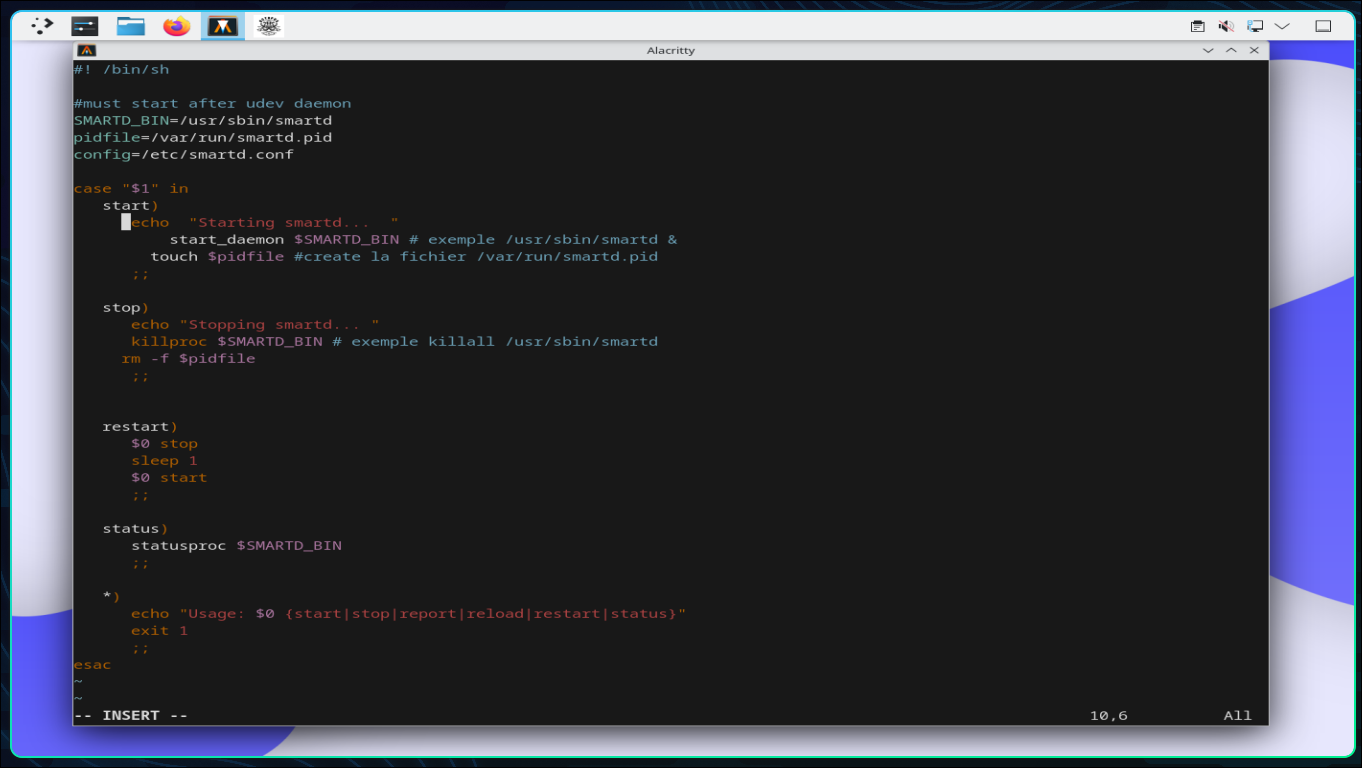
\includegraphics[width=0.85\textwidth]{images_pfe/smartdboots.png}
%  \caption{Script SystemV pour le démon smartd}
%  \label{fig:smartd_bootscript}
%\end{figure}

\section{Bibliothèques générales}
\label{subsec:general-lib}

Exemple  des bibliothèques utilitaires et de support :

\begin{table}[H]
    \centering
    \begin{tabular}{|c|p{8cm}|}
        \hline
        \textbf{Paquet}  & \textbf{Fonction principale} \\
        \hline
        dbus-glib & Liaison GLib pour D-Bus - Intégration des services de bus de messages dans les applications GLib \\
        \hline
        Fontconfig  & Configuration et personnalisation des polices système  \\
        \hline
        
        Wayland & Protocole de serveur d'affichage moderne (alternative à X11) pour la composition graphique \\
        \hline
        
    \end{tabular}
    \caption{Bibliothèques système et de support général}
    \label{tab:general-lib}
\end{table}




%\section{Bibliothèques graphiques et polices}
%\label{subsec:graphics-fonts}

%Paquets pour le rendu graphique et la gestion des polices :

%\begin{table}[H]
%    \centering
%    \begin{tabular}{|c|p{8cm}|}
%        \hline
%        \textbf{Paquet}  & \textbf{Fonction principale} \\
%        \hline
%        FreeType & Moteur de rendu de polices vectorielles \\
%        \hline
%        Fontconfig  & Configuration et personnalisation des polices système  \\
%        \hline
%        
%        Pixman  & Bibliothèque de manipulation de pixels bas niveau pour les opérations graphiques  \\
%        \hline
 %   \end{tabular}
 %   \caption{Bibliothèques graphiques et gestion des polices}
 %   \label{tab:graphics-fonts}
%\end{table}

%\textbf{Exemple d'installation du paquet harfBuzz-9.0.0} :  
%Le paquet HarfBuzz fournit un moteur de mise en forme de texte pour les polices OpenType.

%\textbf{Dépendances de harfBuzz} :
%\begin{verbatim}
%GLib-2.80.4       texlive-20240312   Graphite2-1.3.14   ICU-75.1
%FreeType-2.13.3 
%\end{verbatim}

%\textbf{Remarque} :  
%Ce paquet présente une \textbf{dépendance circulaire} avec FreeType-2.13.3 (bibliothèque de rendu de polices TrueType).  
%La procédure correcte est :  \\
%1. Compiler FreeType  \\
%2. Compiler HarfBuzz  \\
%3. Recompiler FreeType  \\

%\textbf{Exemple de compilation de harfbuzz depuis les sources} :
%\begin{verbatim}
%1: Résoudre toutes les dépendances listées ci-dessus
%2: Télécharger l'archive
%wget https://github.com/harfbuzz/harfbuzz/releases/download/9.0.0/harfbuzz-9.0.0.tar.xz
%3: Vérifier l'intégrité de l'archive
%   md5sum harfbuzz-9.0.0.tar.xz  # Doit être 0035c129cb1646ab1cff65e5ef7153db
%4: Extraire l'archive
%   tar -xvf harfbuzz-9.0.0.tar.xz
%5: Accéder au répertoire
%   cd harfbuzz-9.0.0
%6: Créer un répertoire de compilation
%   mkdir build && cd build
%7: Configurer (système de build : Meson avec Ninja)
%   meson setup ..             \
%      --prefix=/usr           \
%      --buildtype=release     \
%      -D graphite2=enabled 
%8: Compiler
%   ninja
%9: Tester
%   ninja test
%10: Installer
%   ninja install
%11: Nettoyer
%   rm -rf ../../harfbuzz-9.0.0
%\end{verbatim}

%\textbf{Programmes installés} :  
%hb-info, hb-ot-shape-closure, hb-shape, hb-subset, hb-view

%\textbf{Bibliothèques installées} :  
%\begin{itemize}
%  \item \texttt{libharfbuzz.so}
%  \item \texttt{libharfbuzz-cairo.so}
%  \item \texttt{libharfbuzz-gobject.so}
 % \item \texttt{libharfbuzz-icu.so}
 % \item \texttt{libharfbuzz-subset.so}
%\end{itemize}

%\textbf{Documentation} :  
%\texttt{/usr/share/gtk-doc/html/harfbuzz}
%\section{Paquets et bibliothèques réseau}
%\label{subsec:networking}

\section{Composants pour la connectivité et la gestion réseau} 

\begin{table}[H]
    \centering
    \begin{tabular}{|c|p{8cm}|}
        \hline
        \textbf{Paquet}  & \textbf{Fonction principale} \\
        \hline
        NetworkManager  & Gestion dynamique des connexions réseau (Wi-Fi, Ethernet, VPN)  \\
        \hline
       
        Net-tools  & Collection d'outils réseau  (\texttt{ifconfig}, \texttt{netstat}, \texttt{route}) \\
        \hline
    \end{tabular}
    \caption{Composants pour la connectivité et gestion réseau}
    \label{tab:network}
\end{table}



\section{Environnement graphique XORG}

\begin{figure}[H]
  \centering
  \begin{minipage}[b]{0.30\textwidth}
    
\includegraphics[width=\textwidth]{images_pfe/xorg.jpeg}
    \caption{Xorg}
  \end{minipage}\hfill
  \begin{minipage}[b]{0.30\textwidth}
    
\includegraphics[width=\textwidth]{images_pfe/wayland.png}
    \caption{Wayland}
  \end{minipage}
  \caption{Xorg et Wayland}
  \label{fig:xorgwayland}
\end{figure}
\FloatBarrier

Il existe des environnements graphiques sous GNU/Linux :

\begin{itemize}
    \item \textbf{Xorg} : ancien, basé sur une architecture \textbf{client-serveur}.
    \item \textbf{Wayland} : a émergé comme une alternative moderne à Xorg. Il prend en charge de nombreuses animations et personnalisations. Cependant, il dépend fortement des capacités 3D du GPU, ce qui peut entraîner des bugs lorsqu’il est utilisé dans une machine virtuelle.
\end{itemize}

C’est pourquoi nous avons choisi d’implémenter \texttt{Xorg} par défaut dans notre distribution, afin de garantir une \textbf{compatibilité maximale} avec tous les environnements.

\subsection*{Exemples d'applications et bibliothèques Xorg}

\begin{table}[H]
    \centering
    \begin{tabular}{|c|p{8cm}|}
        \hline
        \textbf{Paquet}  & \textbf{Fonction principale} \\
        \hline
        xterm & Émulateur de terminal standard pour Xorg \\
        \hline
        xinit  & Utilitaire de lancement du serveur X et session utilisateur \\
        \hline
        libX11  & Bibliothèque cliente principale X11 (gestion fenêtres/événements) \\
        \hline
        xcursor-themes & Collection d'icônes de curseur pour X11 (thèmes par défaut) \\
        \hline
    \end{tabular}
    \caption{Applications et utilitaires d'entrée Xorg}
    \label{tab:xorg-apps}
\end{table}

\textcolor{blue}{Pour plus d’informations sur Xorg, voir \cite{doc_xorg}.}\\
\textcolor{blue}{Pour plus d’informations sur les bibliothèques Xorg, voir \cite{bibliotheques_xorg}.}

\section{Environnement de bureau}
\label{subsec:desktop-env}


Un environnement de bureau offre une interface plus complète au système d’exploitation, avec un ensemble d’utilitaires et d’applications intégrés.

\textbf{KDE} est un environnement de bureau complet, reposant sur le framework \textbf{Qt}, rassemblant de nombreuses applications et une vaste communauté d’utilisateurs.\\
 KDE  se divise en deux blocs principaux :  
\begin{itemize}
  \item \textbf{KDE Frameworks 6} (KF6)   et \textbf{KDE Plasma 6} 
  
\end{itemize}



\subsection{KDE Frameworks 6}
\label{sssec:kf6}

KDE Frameworks 6 est un ensemble de bibliothèques basées sur Qt 6 et QML

Exemple des  bibliothèques


% KDE Frameworks 6
\begin{table}[H]
    \centering
    \begin{tabular}{|c|p{8cm}|}
        \hline
        \textbf{Paquet}  & \textbf{Fonction principale} \\
        \hline
       
        extra-cmake-modules  & Modules CMake supplémentaires pour la construction des logiciels KDE \\
        \hline
        kapidox  & Outil de génération de documentation API pour les frameworks KDE \\
        \hline
        
    \end{tabular}
    \caption{Composants clés de KDE Frameworks 6}\\
    \label{tab:kf6}
\end{table}

\textcolor{blue}{Pour plusieur information sur kde framework  \cite{framework_kde}}.\\

\subsection{Applications KDE}
\label{sssec:kde-apps}

Pour enrichir l’expérience utilisateur, nous installons plusieurs applications KDE ,Exemple :

\begin{table}[H]
    \centering
    \begin{tabular}{|c|p{8cm}|}
        \hline
        \textbf{Paquet} & \textbf{Fonction principale} \\
        \hline
        konsole  & Terminal émulateur avancé avec onglets et profils personnalisables \\
        \hline
        dolphin & Gestionnaire de fichiers phare de KDE avec navigation par onglets \\
        \hline
        plasma-activities  & Gestion des espaces de travail virtuels et suivi des tâches \\
        \hline
        khelpcenter  & Centre d'aide unifié pour la documentation KDE et manuels \\
        \hline
    \end{tabular}
    \caption{Applications principales de l'écosystème KDE}
    \label{tab:kde-apps}
\end{table}

\subsection{KDE Plasma 6}
\label{sssec:plasma6}

KDE Plasma est un ensemble de paquets construits sur KDE Frameworks et QML, constituant l’environnement d’affichage Plasma.

Exemple des Composants Plasma 6


\begin{table}[H]
    \centering
    \begin{tabular}{|c|p{8cm}|}
        \hline
        \textbf{Paquet}  & \textbf{Fonction principale} \\
        \hline
        kscreenlocker  & Système de verrouillage d'écran sécurisé avec intégration PAM \\
        \hline
        plasma-desktop  & Environnement de bureau principal avec panneau et widgets \\
        \hline
        plasma-workspace  & Couche d'intégration pour la gestion des sessions Plasma \\
        \hline
        breeze  & Thème visuel par défaut de Plasma (icônes, décorations de fenêtre) \\
        \hline
    \end{tabular}
    \caption{Composants fondamentaux de KDE Plasma 6}
    \label{tab:plasma6}
\end{table}

\textcolor{blue}{Pour plusieur information sur kde Plasma   \cite{environnement_plasma}}.\\
\section{Thème KDE Plasma et sélecteur de domaine}
\label{sssec:kde-theme-domain}

Nous avons choisi de personnaliser le thème KDE Plasma pour qu’il reflète l’identité de \textsc{Kraken OS}.  
Cette personnalisation inclut :
\begin{itemize}
  \item la modification du panneau par défaut (couleurs, transparences) ;
  \item l’installation de \texttt{cairo‑dock} pour un lanceur plus ergonomique ;
  \item la création d’environnements visuels distincts pour chaque domaine scientifique (web, mobile, IA/ML, cybersécurité, mathématiques, physique, etc.).
\end{itemize}

Nous avons également développé une application \textbf{simple}, reposant sur les activités KDE Plasma, permettant à l’utilisateur de basculer d’un domaine à l’autre.\\

\begin{figure}[H]
  \centering
  \includegraphics[width=1\textwidth]{images_pfe/defaultswitcher.png}
  \caption{Sélecteur de domaine par défaut de \textsc{Kraken}}
  \label{fig:dks}
\end{figure}

\textcolor{blue}{Pour voir une vidéo de prévisualisation de notre environnement KDE Plasma personnalisé, voir \cite{kde_preview}.}\\

\textcolor{blue}{Le code source de l’application qui permet de changer de domaine est disponible dans \cite{switch_domaine}.}\\
\textcolor{blue}{Pour voir une vidéo de prévisualisation de notre application de changement de domaine, voir \cite{kraken_doamin_switcher}.}\\





 \clearpage

\section{Navigateur web}
\label{subsec:web-browser}

Nous avons choisi d’installer le navigateur \textbf{Firefox}, en raison de sa philosophie open source et de sa simplicité.  
Le navigateur Brave, quant à lui, est un paquet volumineux nécessitant environ 30 Go de données pour sa compilation, car il dépend de Chromium.  
%List des depandances de firefox  :
%\begin{verbatim}
%Cbindgen-0.27.0       GTK+-3.24.43          libnotify-0.8.3   LLVM-18.1.7             
%nodejs-20.16.0        PulseAudio-17.0       Python-3.12.5     startup-notification-0.12
%UnZip-6.0             alsa-lib-1.2.12       SQLite-3.46.1     NASM-2.16.03    
%cURL-8.9.1            Doxygen-1.12.0        FFmpeg-7.0.2      GeoClue-2.7.1            
%liboauth-1.0.3        pciutils-3.13.0       Valgrind-3.23.0    Wget-1.24.5              
%Wireless-Tools-29     yasm-1.3.0            nss-3.103            
%\end{verbatim}
\begin{figure}[H]
  \centering
  \includegraphics[width=1\textwidth]{images_pfe/firefox.png}
  \caption{Navigateur web firefox}
  \label{fig:firefox-custom}
\end{figure}



 
\section{Gestionnaire d’affichage et thème du bootloader GRUB}
\label{subsec:sddm-theme}

\subsection{Thème SDDM}
Un gestionnaire d'affichage (login manager) est une interface graphique lancée au démarrage du système, remplaçant le shell par défaut. 

Pour sa légèreté et sa facilité de personnalisation, nous avons retenu \textbf{SDDM} comme gestionnaire d’affichage.  
Basé sur Qt/QML, il permet une création intuitive de thèmes visuels grâce à son langage déclaratif.

\begin{figure}[H]
  \centering
  \includegraphics[width=1\textwidth]{images_pfe/sddmkrakentheme.png}
  \caption{Thème SDDM personnalisé pour \textsc{Kraken OS}}
  \label{fig:sddm-custom}
\end{figure}

    \textbf{Remarque} : Ce thème, nommé SDDM-Astronaut, est principalement développé par Keyitdev.
Étant donné que le thème est sous licence GPL, nous pouvons le modifier. Nous avons donc apporté des modifications simples\\

\textcolor{blue}{Version originale du thème Astronaut : disponible dans \cite{sddm_theme_astronaut}}.\\
\textcolor{blue}{Notre Version modifiée : disponible dans \cite{sddm_theme_kraken}}.\\
\subsection{Thème GRUB}
\label{subsec:grub-theme}

Le thème GRUB a été adapté à la charte graphique de la distribution. Sa structure minimale comprend :
\begin{itemize}
    \item Un fichier principal \texttt{theme.txt} 
    \item Configuration des polices, couleurs et résolution
   
\end{itemize}



\begin{figure}[H]
  \centering
  \includegraphics[width=1\textwidth]{images_pfe/grubthemekraken.png}
  \caption{Thème GRUB personnalisé pour \textsc{Kraken OS}}
  \label{fig:grub-custom}
\end{figure}

\textcolor{blue}{Code source disponible dans \cite{theme_grub}}.
\section{Conclusion}
À ce stade, nous disposons d'une distribution Linux fonctionnelle et enrichie. Cependant, il manque encore un composant essentiel : un \textbf{gestionnaire de paquets} permettant aux utilisateurs d'installer, mettre à jour ou supprimer des logiciels de manière cohérente.

Dans le prochain chapitre, nous aborderons le développement et l'intégration de notre gestionnaire de paquets 
\chapter{ Gestionnaire de paquets : \textsc{Kraken}s}
\minitoc
\clearpage

\label{sec:pkgmgr}

\section{Introduction}
\label{sec:intro}

Pour résoudre les limitations de compilation , nous avons mis en place un ensemble d'outils, de scripts et de mécanismes dédiés à la gestion des paquets.  
Cela inclut :
\begin{itemize}
    \item Une structure de dépôt simple ;
    \item Un format de fichier \texttt{PKGBUILD.kraken} pour décrire les paquets ;
    \item Des outils CLI personnalisés pour installer, mettre à jour, supprimer ou rechercher des paquets ;
    \item Un système de gestion des dépendances ;
    \item Un mécanisme de suivi des métadonnées des paquets ;
\end{itemize}

\subsubsection*{Langages s utilisés:}
\begin{figure}[hbt!]
  \centering
  \begin{minipage}[b]{0.18\textwidth}
    \includegraphics[width=\textwidth]{images_pfe/c.png}
    \caption{C}
  \end{minipage}\hfill
  \begin{minipage}[b]{0.18\textwidth}
    \includegraphics[width=\textwidth]{images_pfe/bash.jpeg}
    \caption{BASH SCRIPT}
  \end{minipage}\hfill
  \begin{minipage}[b]{0.18\textwidth}
    \includegraphics[width=\textwidth]{images_pfe/yml.png}
    \caption{YAML}
  \end{minipage}\hfill
  \begin{minipage}[b]{0.18\textwidth}
    \includegraphics[width=\textwidth]{images_pfe/sqlite.jpeg}
    \caption{SQLITE3}
  \end{minipage}\hfill
  
  \caption{Stack technique de la gestionnaire des paquetes}
  \label{fig:KPGlanguage}
\end{figure}
\FloatBarrier












Notre gestionnaire de paquets se compose de deux composants principaux :
\begin{enumerate}
    \item Le dépôt où sont stockées les métadonnées des paquets ;
    \item Les outils du gestionnaire interagissant avec ce dépôt.
\end{enumerate}

\section{Le dépôt \textsc{Kraken}}
\label{subsec:depot-kraken}

Le dépôt \textsc{Kraken} contient les métadonnées de tous les paquets disponibles, stockées dans des fichiers \texttt{PKGBUILD.kraken}. Chaque fichier décrit la procédure de compilation d'un paquet à partir des sources.

\subsection{Structure du dépôt }
\label{subsubsec:structure-depot}

La structure du dépôt \textsc{Kraken} est conçue pour être lisible, modulaire et maintenable. Chaque paquet correspond à un dossier contenant un fichier \texttt{PKGBUILD.kraken}.\\



\begin{figure}[H]
  \centering
  \includegraphics[width=1\textwidth]{images_pfe/repodotoff.png}
  \caption{Structure du dépôt du gestionnaire de paquets \textsc{Kraken}}
  \label{fig:krakenrepo}
\end{figure}

Le dépôt comporte quatre catégories principales :
\begin{itemize}
    \item \textbf{core} : Contient les paquets fondamentaux (gcc, binutils, coreutils...) ;
    \item \textbf{extend} : Paquets d'extension pour enrichir le système (xorg, fakroot, strace...) ;
    \item \textbf{sc} : Outils pour l'informatique (applications web, outils mobiles...) ;
    \item \textbf{temps\_tools} : Outils temporaires pour la chaîne de compilation croisée.
\end{itemize}

\textbf{Note} : Des autre catégories comme  \textbf{math} et \textbf{phys} existent également mais ont été omises pour simplifier la figure.

Chaque paquet dans ces répertoires est décrit par un fichier \texttt{PKGBUILD.kraken} spécifiant sa procédure de construction.

\subsection{Le fichier \texttt{PKGBUILD.kraken}}
\label{subsubsec:pkgbuild-file}

Le fichier \texttt{PKGBUILD.kraken} est un modèle déclaratif décrivant :
\begin{itemize}
    \item La méthode de construction du paquet ;
    \item Ses dépendances ;
    \item Son processus d'installation.
\end{itemize}

\begin{figure}[H]
  \centering
  \includegraphics[width=1\textwidth, height=10cm]{images_pfe/pkgbuildkrakenmodle.png}
  \caption{Modèle générique de \texttt{PKGBUILD.kraken}}
  \label{fig:pkgtemplate}
\end{figure}
\clearpage
Exemple concret de \texttt{PKGBUILD.KRAKEN} pour le paquette \texttt{gcc } :
\begin{figure}[H]
  \centering
  \includegraphics[width=1\textwidth, height=10cm]{images_pfe/exemplepgkbuldgcc.png}
  \caption{Exemple de \texttt{PKGBUILD.kraken} pour le paquet \texttt{gcc}}
  \label{fig:pkgbuildgcc}
\end{figure}

Principales sections du fichier :
\begin{itemize}
    \item \textbf{pkgname}, \textbf{pkgver} : Nom et Version  du paquet ;
    \item \textbf{dependencies} : Dépendances requises avant installation ;
    \item \textbf{sources} : lien de téléchargement de l'archive ;
    \item \textbf{md5sums} : Vérification d'intégrité de l'archive ;
    \item \textbf{kraken-prepare()} : Préparation (extraction, configuration) ;
    \item \textbf{kraken-build()} : Compilation du paquet ;
    \item \textbf{kraken-test} : Procédure de test ;
    \item \textbf{kraken-preinstall} : Préconfigurations avant installation ;
    \item \textbf{kraken-install()} : Installation des fichiers système ;
    \item \textbf{kraken-postinstall} : Postconfigurations (documentation, fichiers) ;
    \item \textbf{kraken-remove} : Procédure de désinstallation.
\end{itemize}

\subsection{Le fichier pkgindex.kraken}
\label{subsubsec:pkgindex}
Le fichier \texttt{pkgindex.kraken} est un index centralisé au format YAML qui contient les métadonnées essentielles de tous les paquets disponibles.
\begin{figure}[H]
  \centering
  \includegraphics[width=1\textwidth]{images_pfe/pkgindekrakenpkgindex.png}
  \caption{Exemple de fichier pkgindex.kraken}
  \label{fig:pkgindex-example}
\end{figure}

Chaque entrée de paquet contient les champs suivants :
\begin{itemize}
    \item \textbf{category} : Classification fonctionnelle (core, math, physics, etc.)
    \item \textbf{version} : Version de paquets
    \item \textbf{path} : Chemin relatif vers le fichier \texttt{pkgbuild.kraken} dans le depot.
    \item \textbf{dependencies} : Liste des dépendances obligatoires de ce paquetes
    \item \textbf{checksum} : Vérification d'intégrité  du fichier de \texttt{pkgbuild.kraken} de cette paquetes
\end{itemize}
Ce fichier \textbf{généré automatiquement} optimise la recherche de paquets via :
\begin{itemize}
\item \textbf{Réduction} de la complexité de recherche des paquetes dans le depot  de O(n) à O(1) ;
\item \textbf{Mise à jour} instantanée lors des modifications du dépôt ;
\item \textbf{Accès} hors ligne aux métadonnées (versions, dépendances).
\end{itemize}





\clearpage
\subsection{Résumé de la structure du dépôt}
\label{subsec:resume-depot}

Pour résumer cette section :

\begin{itemize}
    \item Le dépôt est organisé en \textbf{répertoires thématiques} classés par domaine (core, extends, sc, math , phys,etc.) ;
    \item Chaque répertoire contient des paquets spécifiques à son domaine ;
    \item Chaque paquet est décrit par un fichier \texttt{PKGBUILD.kraken} qui :
    \begin{itemize}
        \item Est utilise par le gestionnaire de paquets
        \item Contient les instructions de compilation/installation de cette paquette
    \end{itemize}
    \item Le fichier \texttt{pkgindex.kraken} centralise les métadonnées :
    \begin{itemize}
        \item Noms et versions des paquets
        \item Dépendances entre paquets
       \item \textbf{Liens directs} vers les fichiers pkgbuild.kraken de chaque paquet qui existe dans le dépôt.

        \item Permet une recherche optimisée (complexité O(1)) dans le depot.
    \end{itemize}
\end{itemize}





\textcolor{blue}{Code source de la depot (KUR:kraken users repository) disponible dans  \cite{depot_kur}}.
\section{Les outils \textsc{Kraken}}
\label{subsec:kraken-tools}


\




%-------- kraken tools ------------------







Dans cette section, nous présentons les outils en ligne de commande développés pour gérer les paquets à travers le gestionnaire \textsc{Kraken}. Chaque outil est conçu pour exécuter une étape spécifique du cycle de vie d’un paquet : téléchargement, préparation, compilation, test, etc.


\subsection{kraken help}
\label{subsec:kraken-help}

Cet outil fournit à l'utilisateur un menu d'aide comprenant :
\begin{itemize}
    \item La liste des commandes disponibles
    \item Les paramètres acceptés par chaque commande
    \item Des exemples de workflows d'utilisation

\end{itemize}

\begin{figure}[H]
  \centering
  \includegraphics[width=1\textwidth, height=12cm]{images_pfe/krakenhelpmenu.png}
  \caption{Menu d'aide du gestionnaire de paquets \textsc{Kraken}}
  \label{fig:kraken-help}
\end{figure} 

\subsection{kraken download}

\textbf{Utilisation :} \texttt{sudo kraken download <nom\_du\_paquet>}

Cet outil permet de télécharger l’archive (tarball) d’un paquet et de vérifier son intégrité (via \texttt{md5sum}).

\paragraph{Étapes de fonctionnement :}
\begin{enumerate}
    \item Télécharger ou mettre à jour le fichier \texttt{pkgindex.kraken}, et le stocker dans .cache/kraken/krakenindex
    \item Vérifier que le nom du paquet fourni par l'utilisateur existe dans le dépôt depuit le fichier pkgindex.kraken.
    \item Si le paquet existe, créer un répertoire de compilation nommé \texttt{source/}, puis créer un sous-dossier nommé selon le paquet. Dans ce dossier, télécharger le fichier \texttt{PKGBUILD.kraken} et télécharger l’archive du paquet via le champ sources de la ficher pkgbuild.kraken.
    \item Vérifier l'intégrité du fichier \texttt{PKGBUILD.kraken} ainsi que celle de l’archive téléchargée.
    \item Mettre à jour la base de données \texttt{/var/lib/kraken/kraken.db} en marquant le paquet comme téléchargé.
\end{enumerate}

%\begin{figure}[H]
 % \centering
  %\includegraphics[width=1\textwidth, height=10cm]{images_pfe/downlad.png}
  %\caption{Exemple pratique de l’outil \texttt{kraken download}}
  %\label{fig:pkgtemplate}
%\end{figure}




\subsection{kraken prepare}

\textbf{Utilisation :} \texttt{sudo kraken prepare <nom\_du\_paquet>}

Cet outil est conçu pour préparer le paquet avant sa compilation.

\paragraph{Étapes de fonctionnement :}
\begin{enumerate}
    \item Interroger la base de données pour vérifier si le paquet a été téléchargé.
    \item Si oui, localiser l’archive et l’extraire (en utilisant \texttt{tar}, \texttt{unzip}, etc., selon le format).
    \item Extraire la fonction \texttt{kraken\_prepare()} du fichier \texttt{PKGBUILD.kraken} du paquet, et l’exécuter.
    \item Mettre à jour la base de données en marquant le paquet comme préparé (\texttt{prepared = 1}).
\end{enumerate}

%\begin{figure}[H]
 % \centering
  %\includegraphics[width=1\textwidth, height=10cm]{images_pfe/prepare.png}
  %\caption{Exemple pratique de l’outil \texttt{kraken prepare}}
  %\label{fig:pkgtemplate}
%\end{figure}





\subsection{kraken build}

\textbf{Utilisation :} \texttt{sudo kraken build <nom\_du\_paquet>}

Cet outil est conçu pour compiler les paquets à l’aide de leur système de build (\texttt{make}, \texttt{ninja}, \texttt{meson}, etc.).

\paragraph{Étapes de fonctionnement :}
\begin{enumerate}
    \item Interroger la base de données pour vérifier si le paquet a été préparé.
    \item Si oui,  Extraire la fonction \texttt{build()} du fichier \texttt{PKGBUILD.kraken} et l’exécuter pour compiler le paquet (génération de bibliothèques, binaires, etc.).
    \item Mettre à jour la base de données en marquant le paquet comme compilé (\texttt{built = 1}).
\end{enumerate}







\subsection{kraken test}

\textbf{Utilisation :} \texttt{sudo kraken test <nom\_du\_paquet>}

\paragraph{Étapes de fonctionnement :}
\begin{enumerate}
    \item Interroger la base de données pour vérifier si le paquet a été compilé.
    \item Si oui, Extraire la fonction \texttt{test()} depuis le fichier \texttt{PKGBUILD.kraken}, et l’exécuter afin de tester le paquet compilé.
\end{enumerate}

\textbf{Remarque :} les tests sont optionnels. Certains paquets ne fournissent pas de suite de test officielle, donc l'exécution de cette étape n'est pas considérée comme critique.

%\begin{figure}[H]
 % \centering
 % \includegraphics[width=1\textwidth, height=10cm]{images_pfe/test.png}
 % \caption{Exemple pratique de l’outil \texttt{kraken test}}
 % \label{fig:pkgtemplate}
%\end{figure}










\subsection*{Principe de la « fausse installation »}  
\label{subsecc:fakeinstall}
Comme nous l'avons vu dans le chapitre \ref{subsec:suivi-fichiers}, nous devons implémenter un mécanisme qui installe les paquets de manière fictive dans un répertoire temporaire afin de détecter tous les fichiers et répertoires créés par le paquet lors de l'installation. Cette étape sera utilisée ultérieurement dans le mécanisme de suppression des paquets.

\textbf{Utilisation :} \texttt{sudo kraken fakeinstall <nom\_du\_paquet>}

\textbf{Étapes :}
\begin{enumerate}
  \item Vérifier si le paquet a été compiler  ou non à partir de la base de données.
  \item Si oui, Extraire la fonction \texttt{kraken-install} du fichier \texttt{pkgbuild.kraken} et créer un répertoire temporaire situé dans \texttt{/tmp} où le paquet sera installé \textbf{fictivement}, en forçant l’installation dans ce répertoire de destination.
  \item Créer un environnement fictif à l’aide de l’outil \textbf{fakeroot}.
  \item Lancer l’installation du paquet  en parallèle avec l’outil \textbf{strace} afin de détecter tous les changements effectués sur le système.
  \item Générer les métadonnées dans :
  \begin{itemize}
    \item \texttt{/var/lib/kraken/packages/DIRS} -- contient tous les répertoires marqués par le paquet.
    \item \texttt{/var/lib/kraken/packages/FILES} -- contient tous les fichiers marqués par le paquet.
  \end{itemize}
\end{enumerate}

%La figure suivante montre un exemple pratique de l'utilisation de l’outil \texttt{fakeinstall} :

%\begin{figure}[H]
%  \centering
 % \includegraphics[width=1\textwidth, height=10cm]{images_pfe/pkgbuildkrakenmodle.png}
  %\caption{Modèle de fichier \texttt{pkgbuild.kraken}}
  %\label{fig:pkgtemplate}
%\end{figure}


%\textcolor{red}{Cette figure illustre un exemple des fichiers et répertoires de métadonnées générés pour un paquet (\texttt{DIRS} et %\texttt{FILES}) :}

%\begin{figure}[H]
%  \centering
%  \includegraphics[width=1\textwidth, height=10cm]{images_pfe/pkgbuildkrakenmodle.png}
%  \caption{Modèle de fichier \texttt{pkgbuild.kraken}}
%  \label{fig:pkgtemplate}
%\end{figure}

%\textbf{Remarque :} Comme vous pouvez le voir dans la figure, les fichiers \texttt{DIRS} et \texttt{FILES} contiennent certains répertoires %critiques tels que \texttt{/usr}, \texttt{/boot}, \texttt{/bin}, \texttt{/root}. Il est donc nécessaire de mettre en place un mécanisme de %filtrage de ces répertoires afin de garantir que le système de fichiers critique ne soit pas altéré lors de la suppression d’un paquet.





\subsection{kraken install}

\textbf{Utilisation :} \texttt{sudo kraken install <nom\_du\_paquet>}

Cet outil est conçu pour installer les paquets dans le système final.

\textbf{Étapes :}
\begin{enumerate}
  \item Vérifier si le paquet a été installé fictivement (fakeinstall) dans la base de données.
  \item Si oui, Exécuter la fonction \texttt{install} située dans le fichier \texttt{pkgbuild.kraken}.
  \item Marquer le paquet comme installé définitivement dans le système avec la date d’installation.
\end{enumerate}



%\begin{figure}[H]
%  \centering
%  \includegraphics[width=1\textwidth, height=10cm]{images_pfe/install.png}
%  \caption{Modèle de fichier \texttt{pkgbuild.kraken}}
%  \label{fig:pkgtemplate}
%\end{figure}





\subsection{kraken postinstall}

\textbf{Utilisation :} \texttt{sudo kraken postinstall <nom\_du\_paquet>}

Cet outil est conçu pour exécuter les configurations post-installation après l’installation du paquet, comme la modification de certains fichiers de configuration.

\textbf{Étapes :}
\begin{enumerate}
  \item Vérifier si le paquet est installé dans le système en consultant la base de données.
  \item Si oui, Exécuter la fonction \texttt{postinstall} à partir du fichier \texttt{pkgbuild.kraken}.
\end{enumerate}

%La figure suivante montre un exemple d’utilisation de l’outil \texttt{postinstall} :

%\begin{figure}[H]
%  \centering
 % \includegraphics[width=1\textwidth, height=10cm]{images_pfe/alpine.jpg}
 % \caption{Modèle de fichier \texttt{pkgbuild.kraken}}
 % \label{fig:pkgtemplate}
%\end{figure}
%\textcolor{blue}{Pour voir une vidéo de démonstration de l’utilisation de ces outils pour installer un paquet, voir \cite{kraken_tools}.}

\subsection{kraken remove}

\textbf{Utilisation :} \texttt{sudo kraken remove <nom\_du\_paquet>}

Ce mécanisme prend en charge deux cas :

\begin{enumerate}
  \item Détecter si le paquet possède un mécanisme de désinstallation dans son système de construction. Si oui, nous l’utilisons pour supprimer le paquet.
  \item Si le paquet ne possède pas de mécanisme de désinstallation, nous appelons un mécanisme nommé \texttt{manual\_install}. Celui-ci parcourt les fichiers de métadonnées (\texttt{FILES}, \texttt{DIRS}) créés lors de l’étape \texttt{fakeinstall}, et supprime tous les fichiers et répertoires listés.
  \item Mettre à jour la base de données en supprimant le paquet de la table des paquets installés.
\end{enumerate}



%\begin{figure}[H]
 % \centering
  %\includegraphics[width=1\textwidth, height=10cm]{images_pfe/pkgbuildkrakenmodle.png}
  %\caption{Modèle de fichier \texttt{pkgbuild.kraken}}
  %\label{fig:pkgtemplate}
%\end{figure}

\subsection{kraken entropy}

\textbf{Utilisation :} \texttt{sudo kraken entropy <nom\_du\_paquet>}

Cet outil est conçu pour installer \textbf{automatiquement} le paquet ainsi que toutes ses dépendances.

\textbf{Étapes :}
\begin{enumerate}
  \item Construire le graphe complet du paquet, affichant toutes les dépendances et les dépendances des dépendances.
  \item Détecter s'il y a des cycles dans le graphe ou des dépendances de type config ou diamant. Pour en savoir plus sur ces problèmes, référez-vous au section \textcolor{blue}{\ref{subsec:circular-dependencies}}.
  \item Parcourir le graphe en utilisant la recherche en profondeur (Depth First Search) et installer chaque paquet dans le bon ordre en utilisant les outils précédents (\texttt{download}, \texttt{prepare}, \texttt{build}, \texttt{test}, \texttt{fakeinstall}, \texttt{install}, \texttt{postinstall}).
\end{enumerate}

%Exemple illustrant le mécanisme d'entropie :

%\begin{figure}[H]
 % \centering
 % \includegraphics[width=1\textwidth, height=13cm]{images_pfe/phpgraph.png}
 % \caption{Modèle de fichier \texttt{pkgbuild.kraken}}
 % \label{fig:pkgtemplate}
%\end{figure}


\subsection{kraken getversion}

\textbf{Utilisation :} \texttt{sudo kraken getversion <nom\_du\_paquet>}

Cet outil est conçu pour afficher la version d'un paquet, qu'il soit installé ou non ( depuis le dépôt).


\subsection{kraken dependency}

\textbf{Utilisation :} \texttt{sudo kraken getdeps <nom\_du\_paquet> <version\_du\_paquet>}

Généralement, si vous choisissez de construire le paquet manuellement, vous devez vérifier ses dépendances. Cet outil affiche les dépendances d'un paquet en utilisant \texttt{yq} pour interroger le \texttt{pkgindex.kraken}.



\subsection{kraken checkinstaller}

\textbf{Utilisation :} \texttt{sudo kraken checkinstalled <nom\_du\_paquet>}

Cet outil détecte si le paquet est installé dans le système ou non en interrogeant la base de données.

 
\subsection{Outils en développement}

Comme vous pouvez le voir, notre gestionnaire de paquets construit le paquet à partir des sources, mais nous prévoyons d'améliorer cette fonctionnalité dans les futures versions. Nous préparons le développement d'un mécanisme pour :\\

  permettant de compiler le paquet à l'intérieur de Kraken OS, hébergé dans une machine virtuelle sur un serveur cloud. L'idée est de générer un nouveau tarball \textbf{reconstruit} nommé \texttt{pkgnam-pkgversion.kraken}.\\
Ce tarball sera compilé et configuré dans le cloud, et l'utilisateur n'aura qu'à l'installer sur son système sans avoir à le compiler lui-même.
Cela permettra de réduire le temps de compilation, car la construction de paquets à partir des sources est fastidieuse et consomme beaucoup de ressources et de temps. Par exemple, compiler un paquet comme \texttt{gcc} peut prendre 4 heures avec 6 cœurs.\\

\bigbreak

\textcolor{blue}{Code source  de notre gestionnaires de paquetes kraken  disponible dans  \cite{gestionnaire_paquets}}.\\
\bigbreak
\textcolor{blue}{Pour voir une vidéo de démonstration de l’utilisation de ces outils pour installer un paquet manuellement, voir \cite{kraken_tools}.}\\
\bigbreak
\textcolor{blue}{Pour voir une vidéo de démonstration de l’utilisation de loutil, \texttt{kraken-entropy}, pour installer \textbf{automatiquement} un paquet avec \textbf{la résolution de ses dépendances}, voir \cite{kraken_entropy}.}\\
\bigbreak
\section{Conclusion}
Notre distribution atteint désormais un stade fonctionnel complet, incluant un gestionnaire de paquets \textbf{basique}.\\
La prochaine phase  produire une ISO installable pour permettre son déploiement massif.

\chapter{  Création de l'ISO : Génération de l'image installable}
\minitoc
\clearpage
%\section{Création de l'ISO : Génération de l'image installable}




\section{Introduction}

Afin de rendre le système accessible à l'utilisateur final, nous devons créer une image ISO amorçable que celui-ci pourra télécharger et installer sur sa machine, que ce soit en environnement virtuel ou sur du matériel physique.

La création d’une image ISO est une tâche souvent complexe, tout comme la construction du système lui-même.

\begin{figure}[H]
  \centering
  \includegraphics[width=1\textwidth, height=10cm]{images_pfe/bootloader process.png}
  \caption{Processus de démarrage de Kraken OS}
  \label{fig:kbootproc}
\end{figure}

Lors de l’allumage du PC, un signal électrique déclenche le \textbf{POST} (\emph{Power-On Self-Test}), qui initialise le périphérique de démarrage (BIOS ou UEFI).\\

Ensuite, le BIOS/UEFI charge le chargeur d’amorçage (Syslinux) en lisant le fichier de configuration \texttt{isolinux.cfg}, ce qui permet de charger le noyau Linux (\texttt{vmlinuz-kraken}) ainsi que le disque RAM initial (\texttt{initrd}).

Ainsi, pour créer l'ISO, nous devons suivre les étapes suivantes~:
\begin{itemize}
    \item Générer le fichier SquashFS contenant notre système de fichiers
    \item Développer l'image \texttt{initrd}
    \item Configurer le chargeur d'amorçage Syslinux
    \item Développer un script et une application graphique d'installation pour les utilisateurs
    \item Générer le fichier ISO amorçable
\end{itemize}


\section{Générer le fichier SquashFS}

Depuis le chapitre \ref{chap:corebuild}, nous avons construit notre système sur un disque dur, précisément sur un disque VDI de VirtualBox. Ainsi, pour générer l'ISO, nous devons~:
\begin{itemize}
    \item Convertir ce disque VDI en fichier img au format RAW
    \item Monter le fichier (qui contient déjà plusieurs partitions) à l'aide d'outils comme \texttt{kpartx}
    
\end{itemize}

Nous devons ensuite~:
\begin{itemize}
    \item Nettoyer les fichiers de la partition montée (suppression des fichiers temporaires)
    \item Modifier les configurations système (Exemple  le fichier \texttt{/etc/fstab})
    
\end{itemize}

Enfin, nous générons le fichier SquashFS à l'aide de l'outil \texttt{mksquashfs}. Ce fichier contiendra l'intégralité du système dans un format compressé. Nous utilisons l'algorithme de compression \texttt{xz} pour optimiser l'espace.

\begin{figure}[H]
  \centering
  \includegraphics[width=1\textwidth]{images_pfe/rootfsfile.png}
  \caption{Fichier SquashFS généré}
  \label{fig:rootfs}
\end{figure}



\section{Image initrd}

Nous devons maintenant générer l’image \texttt{initrd}.  
Cette image est développée en utilisant \texttt{BusyBox}, une suite logicielle regroupant plusieurs utilitaires Unix dans un seul fichier exécutable.

\noindent
Nous avons besoin que \texttt{BusyBox} prenne en charge les boucles (\texttt{loop}), \texttt{SquashFS} et d’autres fonctionnalités nécessaires.

\begin{figure}[H]
  \centering
  \includegraphics[width=1\textwidth, height=10cm]{images_pfe/busyboxbinary.png}
  \caption{Structure de l'exécutable BusyBox}
  \label{fig:busybox}
\end{figure}

Cet \texttt{initrd} contient un script d’initialisation nommé \texttt{init}, essentiel au montage du fichier \texttt{SquashFS}. Ce script est écrit en \texttt{Bash} et fonctionne exclusivement sur \texttt{Kraken OS}.

\vspace{0.5cm}
\noindent
\textbf{Exemple du contenu du script \texttt{init} :}
\begin{figure}[H]
  \centering
  \includegraphics[width=1\textwidth, height=10cm]{images_pfe/intirdinitscript.png}
  \caption{Exemple de script \texttt{init}}
  \label{fig:initscript}
\end{figure}

\vspace{0.3cm}
\noindent
\textbf{Explication :}

L’objectif principal de ce script est de :
\begin{enumerate}
  \item Monter les systèmes de fichiers virtuels (\texttt{proc}, \texttt{dev}, \texttt{sys}, etc.) ;
  \item Monter le contenu du fichier ISO dans \texttt{/mnt/iso}, qui contient notre fichier \texttt{squashfs} ;
  \item Monter le fichier \texttt{squashfs}, contenant notre système de fichiers, dans \texttt{/mnt/live} ;
  \item Copier le contenu de \texttt{squashfs} depuis \texttt{/mnt/live} vers \texttt{/mnt/rootfs} ;
  \item Entrer dans l’environnement \texttt{chroot} situé dans \texttt{/mnt/rootfs} à l’aide de la commande \texttt{switch\_root}.
\end{enumerate}

\vspace{0.5cm}
\noindent
\textbf{Remarque :}

Vous vous demandez peut-être pourquoi nous montons le contenu du fichier \texttt{squashfs} à l’étape 3, puis en copions le contenu à l’étape 4.

C’est parce que la philosophie du système de fichiers \texttt{SquashFS} repose sur le principe du \textbf{mode lecture seule}.  
Pour pouvoir effectuer un \texttt{chroot} dans ce système, il aurait fallu monter le fichier \texttt{squashfs} via un système de fichiers de type \texttt{overlay}.

Cela nécessiterait :
\begin{itemize}
  \item De compiler notre noyau avec le support d’\texttt{overlayfs} ;
  \item De compiler \texttt{BusyBox} avec le support du type \texttt{overlay}.
\end{itemize}

Malheureusement, nous n’avons pas eu le temps de mettre en œuvre cette solution.

Nous avons donc choisi une autre approche :  
Monter le fichier \texttt{squashfs} via un \texttt{bind} dans un répertoire, puis copier son contenu dans un autre répertoire accessible en écriture.  
Ce n’est pas la méthode la plus optimale, mais elle est fonctionnelle pour cette version.  
Nous prévoyons d’améliorer cette partie dans une prochaine version de l’image ISO.

\vspace{0.5cm}
\noindent
Après cela, nous générons le fichier \texttt{initrd} à l’aide des outils \texttt{find}, \texttt{cpio}, \texttt{gzip}, etc.

\begin{figure}[H]
  \centering
  \includegraphics[width=1\textwidth, height=10cm]{images_pfe/initrdcontentfile.png}
  \caption{Contenu du fichier \texttt{initrd}}
  \label{fig:initcontent}
\end{figure}

\noindent
\textcolor{blue}{Le code source du fichier \texttt{initrd} et du script \texttt{init} est disponible dans \cite{initrd}.}


\section{Bootloader Syslinux}

Dans l'environnement ISO, il est recommandé d'utiliser le chargeur de démarrage Syslinux au lieu de GRUB pour des raisons de simplicité. Ensuite, pendant l'installation du système depuis l'environnement live vers le disque désiré, nous utiliserons le chargeur de démarrage GRUB. 

Il y a une configuration critique à effectuer dans Syslinux pour garantir un démarrage correct.\\
Exemple du fichier \texttt{isolinux.cfg} :

\begin{figure}[H]
  \centering
  \includegraphics[width=1\textwidth, height=10cm]{images_pfe/cfgisolinuxcorrect.png}
  \caption{Exemple fichier isolinux.cfg }
  \label{fig:isolinux}
\end{figure}

Exemple de menu de syslinux bootloader :

\begin{figure}[H]
  \centering
  \includegraphics[width=1\textwidth, height=10cm]{images_pfe/syslinuxmenu.png}
  \caption{Menu de démarrage Syslinux}
  \label{fig:syslinux}
\end{figure}
\textcolor{blue}{Pour en savoir plus sur syslinux, référez-vous à \cite{syslinux}.}\\
\section{Script d'installation }
\label{secc:sctipttui}

Après avoir démarré l'ISO , nous devons fournir à l'utilisateur un script capable d'installer l'ISO depuis \textbf{l'environnement live} vers le \textbf{disque dur local}.

Ce script gère plusieurs aspects, tels que la partition du disque, le montage du disque, la copie des fichiers système, la configuration du chargeur de démarrage dans le nouveau système, la création d'un utilisateur, la configuration de la langue, de la disposition du clavier, la configuration de l'environnement du nouvel utilisateur, l'édition du fichier \texttt{/etc/fstab}, l'activation de thèmes pour GRUB, SDDM, etc.

Ce script est développé spécialement pour Kraken OS ; si vous tentez de l'exécuter sur une autre machine ou distribution, il échouera.




\textbf{Commande :}

\begin{lstlisting}
./kraken_install.sh "disk_name" "home_on" "swap_on" "username" "userpass" 
  "system_language" "keyboard_layout" "hostname" "time_zone"
\end{lstlisting}

\textbf{Exemple d'utilisation :}
\begin{lstlisting}
sudo ./kraken_install.sh /dev/sda yes yes n1cef password en_US.UTF-8 us kraken /Africa/Tunis
\end{lstlisting}



\textbf{Exemple de parametre valide }
\begin{table}[H]
    \centering
    \small
    \begin{tabularx}{\textwidth}{|c|c|X|}
        \hline
        \textbf{Paramètre} & \textbf{Exemples} & \textbf{Description} \\
        \hline
        \texttt{disk-name} & \texttt{/dev/sda}, \texttt{/dev/sdb} & Chemin complet vers le disque cible \\
        \hline
        \texttt{home-on} & \texttt{yes}, \texttt{no} & Créer une partition séparée pour \texttt{/home} \\
        \hline
        \texttt{swap-on} & \texttt{yes}, \texttt{no} & Créer une partition de swap \\
        \hline
        \texttt{username} & \texttt{n1cef} & Nom du compte utilisateur principal  \\
        \hline
        \texttt{userpass} & \texttt{"MotDePasse123!"} & Mot de passe de l'utilisateur principal  \\
        \hline
        \texttt{system-language} & \texttt{fr-FR.UTF-8}, \texttt{en-US.UTF-8}, \texttt{ar-SA.UTF-8} & Langue et paramètre régional du système \\
        \hline
        \texttt{keyboard-layout} & \texttt{fr}, \texttt{us}, \texttt{ar} & Code de disposition du clavier (Français, Anglais, Arabe) \\
        \hline
        \texttt{hostname} & \texttt{kraken} & Nom d'hôte du système  \\
        \hline
        \texttt{time-zone} & \texttt{/Europe/Paris}, \texttt{/Africa/Tunis}, \texttt{/Asia/Dubai} & Fuseau horaire au format \texttt{/Région/Ville} \\
        \hline
    \end{tabularx}
    \caption{Paramètres de configuration système}
    \label{tab:system-config-params}
\end{table}


%\begin{figure}[H]
 % \centering
 % \includegraphics[width=1\textwidth, height=14cm]{images_pfe/diskuses.png}
 % \caption{ exemple d utilisation de script d’installation }
 % \label{fig:diskuses}
%\end{figure}



\textcolor{blue}{Le code source du script d’installation est disponible dans  \cite{installateur_tui}.}


\section{Application graphique "Kraken Installer" }
\label{secc:graphapp}


Le script d'installation Kraken créé précédemment peut être difficile à utiliser pour un utilisateur Linux non expert. Ainsi, nous avons choisi de développer une application graphique pour rendre le processus d'installation du système plus convivial.




Cette application fournit simplement à l'utilisateur des champs et des options pour sélectionner la langue du système, configurer son nom d'utilisateur et son mot de passe, choisir la disposition du clavier, sélectionner le disque et la partition, choisir les paquets à installer dans le nouveau système, etc.

\textbf{Fonctionnalité clé} : Génération d'un fichier JSON stockant toutes ces configurations pour l'installation ultérieure du système.


\begin{figure}[H]
  \centering
  \includegraphics[width=1\textwidth, height=10cm]{images_pfe/jsonsettings.png}
  \caption{Exemple de fichier settings.json généré}
  \label{fig:jsonsettings}
\end{figure}


\clearpage
\subsection*{Langages et frameworks utilisés}
\begin{figure}[hbt!]
  \centering
  \begin{minipage}[b]{0.18\textwidth}
    \includegraphics[width=\textwidth]{images_pfe/c+++.png}
    \caption{C++17/20}
  \end{minipage}\hfill
  \begin{minipage}[b]{0.18\textwidth}
    \includegraphics[width=\textwidth]{images_pfe/xml.png}
    \caption{Qt XML}
  \end{minipage}\hfill
  \begin{minipage}[b]{0.18\textwidth}
    \includegraphics[width=\textwidth]{images_pfe/qt6.jpeg}
    \caption{Qt6 Framework}
  \end{minipage}\hfill
  \begin{minipage}[b]{0.18\textwidth}
    \includegraphics[width=\textwidth]{images_pfe/css.jpeg}
    \caption{Qt CSS}
  \end{minipage}\hfill
  \caption{Stack technique de l'installateur graphique}
  \label{fig:krakenistallerlanguage}
\end{figure}
\FloatBarrier
 
  
  
  
 


\subsection{ Les pages de l'application}


\subsection{ Page principale}
\begin{figure}[H]
  \centering
  \includegraphics[width=1\textwidth, height=10cm]{images_pfe/mainwindow.png}
  \caption{Page principale de l'application Kraken Installer (page d'accueil)}
  \label{fig:mwindow}
\end{figure}



%\subsection{ Page de bienvenue}

%\begin{figure}[H]
 % \centering
 % \includegraphics[width=1\textwidth, height=10cm]{images_pfe/welcome.png}
 % \caption{Page de bienvenue de l'application Kraken Installer}
 % \label{fig:wlecompage}
%\end{figure}




\subsection{Page de configuration du clavier}
\begin{figure}[H]
  \centering
  \includegraphics[width=1\textwidth, height=10cm]{images_pfe/keyboard.png}
  \caption{Interface de configuration clavier de l'application \textsc{Kraken Installer}}
  \label{fig:keyboardpage}
\end{figure}

\textbf{Fonctionnalité} : Cette page propose à l'utilisateur :
\begin{itemize}
    \item Deux menus déroulants (\texttt{QComboBox}) pour :
    \begin{itemize}
        \item Sélectionner la langue du système
        \item Choisir la disposition du clavier
    \end{itemize}
    \item Un bouton de validation qui :
    \begin{itemize}
        \item Sauvegarde les paramètres dans un fichier \texttt{JSON}
        \item Redirige vers la page suivante
    \end{itemize}
\end{itemize}



\subsection{ Page de configuration de la localisation}

\begin{figure}[H]
  \centering
  \includegraphics[width=1\textwidth, height=10cm]{images_pfe/location.png}
  \caption{Interface de configuration géographique de l'application \textsc{Kraken Installer}}
  \label{fig:locationpage}
\end{figure}

\textbf{Fonctionnalité} : Cette page permet à l'utilisateur de :
\begin{itemize}
    \item Sélectionner sa région géographique via un \texttt{QListWidget}
    \item Choisir son fuseau horaire (ex: \texttt{Africa/Tunis}) via un \texttt{QComboBox}
    \item Valider ces paramètres avec un bouton \textit{Suivant} qui :
    \begin{itemize}
        \item Sauvegarde les configurations dans le fichier \texttt{JSON}
        \item Redirige vers l'étape suivante de l'installation
    \end{itemize}
\end{itemize}



\subsection{Page de configuration de l'utilisateur}

\begin{figure}[H]
  \centering
  \includegraphics[width=1\textwidth, height=10cm]{images_pfe/user.png}
  \caption{Interface de configuration utilisateur de l'application \textsc{Kraken Installer}}
  \label{fig:userpage}
\end{figure}


\textbf{Fonctionnalité} : Cette interface permet à l'utilisateur de :
\begin{itemize}
    \item Définir le nom d'hôte du système via un \texttt{QLineEdit}
    \item Créer un compte utilisateur avec :
    \begin{itemize}
        \item Un champ \texttt{QLineEdit} pour le nom d'utilisateur
        \item Deux champs de mot de passe (saisie + confirmation)
    \end{itemize}
    \item Valider via un bouton \textit{Suivant} qui :
    \begin{itemize}
        \item Vérifie la concordance des mots de passe
        \item Signale les champs incomplets
        \item Sauvegarde les paramètres dans le fichier \texttt{JSON}
        \item Redirige vers l'étape suivante
    \end{itemize}
\end{itemize}

\textbf{Note de sécurité} : 
\begin{itemize}
    \item Les mots de passe doivent être identiques
    \item Tous les champs sont obligatoires
    \item En cas d'erreur, l'application bloque la progression et demande une correction
\end{itemize}



\subsection{Page de partitionnement du disque}

\begin{figure}[H]
  \centering
  \includegraphics[width=1\textwidth, height=10cm]{images_pfe/disk.png}
  \caption{Interface de partitionnement de disque de l'application \textsc{Kraken Installer}}
  \label{fig:diskpage}
\end{figure}

\label{subsec:disk-partitioning}

\textbf{Fonctionnalités} :
\begin{itemize}
    \item \texttt{QTreeWidget} détectant automatiquement les disques disponibles
    \item Bouton \textit{Actualiser les disques} (\texttt{QPushButton}) pour mettre à jour la liste des disques 
    \item Options de partitionnement via des cases à cocher (\texttt{QCheckBox}) :
    \begin{itemize}
        \item Créer une partition \texttt{/home} séparée
        \item Activer une partition \texttt{swap}
        \item Case obligatoire :  Je confirme avoir compris que toutes les données du disque seront effacées
    \end{itemize}
    \item Validation via bouton \textit{Suivant} qui :
    \begin{itemize}
        \item Vérifie la sélection de la case de confirmation
        \item Sauvegarde la configuration dans le fichier \texttt{JSON}
        \item Redirige vers l'étape suivante
    \end{itemize}
\end{itemize}

\


\subsection{Page de sélection des paquets}



\label{subsec:package-selection}
\begin{figure}[H]
  \centering
  \includegraphics[width=1\textwidth, height=10cm]{images_pfe/packages.png}
  \caption{Interface de sélection des paquets de l'application \textsc{Kraken Installer}}
  \label{fig:packagepage}
\end{figure}



\textbf{Fonctionnalités} :  
Cette interface propose à l'utilisateur :
\begin{itemize}
    \item 3 onglets thématiques via \texttt{QTabWidget} :
    \begin{itemize}
        \item Informatique
        \item Mathématiques
        \item Physique
    \end{itemize}
    
    \item Sous-catégories détaillées (exemple pour l'onglet \textit{Informatique}) :
    \begin{itemize}
        \item Outils de développement général
        \item Outils web
        \item DevOps \& Cloud
        \item Développement mobile
        \item Cybersécurité
        \item IA/ML (Intelligence Artificielle et Machine Learning)
    \end{itemize}
    
    \item Sélection via \texttt{QCheckBox} pour chaque paquet
    \item Validation via \texttt{QPushButton} qui :
    \begin{itemize}
        \item Sauvegarde les sélections dans un tableau JSON
        \item Redirige vers l'étape suivante
    \end{itemize}
\end{itemize}





\subsection{Page de progression de l'installation}
\label{subsec:installation-progress}

\begin{figure}[H]
  \centering
  \includegraphics[width=1\textwidth, height=10cm]{images_pfe/installation.png}
  \caption{Interface de progression de l'installation dans \textsc{Kraken Installer}}
  \label{fig:install-page}
\end{figure}

\textbf{Fonctionnalités} :
\begin{itemize}
    \item Bouton \textit{Démarrer l'installation} (\texttt{QPushButton}) lançant le processus :
    \begin{itemize}
        \item Extraction des paramètres  depuis le fichier \texttt{JSON}
        \item Exécution d'un script dinstallation  \textcolor{blue}{\ref{secc:sctipttui}}   avec les paramètres en entrée
    \end{itemize}
    
    \item Widget \texttt{QPlainTextEdit} affichant :
    \begin{itemize}
        \item Les logs d'installation en temps réel
        \item La progression des étapes (partitionnement, copie des fichiers, configuration...)
        
    \end{itemize}
    
    \item Gestion visuelle de la progression :
    \begin{itemize}
        \item Barre de progression intégrée 
       
    \end{itemize}
\end{itemize}




\subsection{Page de redémarrage}


\begin{figure}[H]
  \centering
  \includegraphics[width=1\textwidth, height=10cm]{images_pfe/finish.png}
  \caption{Interface de confirmation de redémarrage dans \textsc{Kraken Installer}}
  \label{fig:reboot-page}
\end{figure}
\label{subsec:reboot}

\textbf{Fonctionnalité finale} :
\begin{itemize}
    \item Bouton de confirmation (\texttt{QPushButton}) demandant à l'utilisateur :
    \begin{itemize}
        \item De valider le redémarrage du système
        
    \end{itemize}
 
 \end{itemize}




\textcolor{blue}{Le code source du  lapplication  graphique d’installation est disponible dans  \cite{installateur_gui}.}
\subsection{ISO}

Maintenant, après avoir préparé tous les composants, on peut générer l'image ISO.\


\medskip
\clearpage
\textbf{Exemple de structure d'un fichier ISO :}

\begin{figure}[H]
  \centering
  \includegraphics[width=1\textwidth, height=10cm]{images_pfe/isocontent.png}
  \caption{Contenu du fichier ISO avant sa génération}
  \label{fig:iso_directory_content}
\end{figure}

\medskip

\textbf{Explication :}\\
Comme le montre la figure, à la racine du répertoire, nous avons le fichier \texttt{squashfs} généré précédemment ainsi qu'un répertoire nommé \texttt{boot}.\\
Dans ce répertoire \texttt{boot}, on trouve les fichiers \texttt{initrd.img}, l’image du noyau, les fichiers \texttt{config} et \texttt{System.map}, ainsi qu’un dossier \texttt{isolinux} contenant notre chargeur d’amorçage (SYSLINUX).\\
Ce dossier \texttt{isolinux} contient des fichiers critiques comme \texttt{isolinux.cfg} \textcolor{blue}{(créé précédemment \ref{fig:isolinux})}, ainsi que plusieurs bibliothèques et modules d’amorçage tels que \texttt{poweroff.c32}, \texttt{reboot.c32}, \texttt{libutil.c32} et \texttt{libmenu.c32}.

\medskip
\bigbreak

\textbf{Exemple de commande pour générer une ISO amorçable :}

\textbf{Remarque :} les grandes distributions créent généralement leurs propres outils pour la génération d'images ISO.\\
Par exemple, la distribution Arch Linux utilise son propre outil appelé \texttt{archiso}, tandis que la distribution Red Hat utilise \texttt{lorax}.\\
Malheureusement, nous n'avons pas encore eu le temps de développer notre propre outil, mais nous envisageons de le faire bientôt.\\
À ce stade, nous utilisons des outils comme \texttt{xorriso} et \texttt{mkisofs} pour générer l'ISO.
\begin{verbatim}
sudo mkisofs \
  -V "KRAKEN-OS" \
  -o /home/nacef/krakenos-3.10.iso \
  -b boot/isolinux/isolinux.bin \
  -c boot/isolinux/boot.cat \
  -no-emul-boot \
  iso-pfe-off
\end{verbatim}

\textbf{Explication des options :}
\begin{itemize}
  \item \texttt{-V "KRAKEN-OS"} : définit l'étiquette de l'ISO
  \item \texttt{-o} : chemin de sortie du fichier ISO
  \item \texttt{-b} : image de démarrage de isolinux
  \item \texttt{-c} : fichier catalogue de démarrage de isolinux
  \item \texttt{-no-emul-boot} : requis pour rendre l’image amorçable
  \item \texttt{iso-pfe-off} : répertoire contenant la structure du système de fichiers ISO
\end{itemize}

\medskip

\textbf{Exemple : détection du type, de la taille et de l’intégrité de l’image ISO à l’aide des commandes \texttt{file}, \texttt{du}, et \texttt{md5sum} :}

\begin{figure}[H]
  \centering
  \includegraphics[width=1\textwidth, height=10cm]{images_pfe/fileisoofff.png}
  \caption{Type du fichier ISO, taille et vérification d'intégrité}
  \label{fig:iso_type}
\end{figure}

\medskip
\textbf{Résumé :}\\
Lorsque l'ISO est démarrée (ex: machine virtuelle), le BIOS/UEFI charge le bootloader ISOLINUX (dans \texttt{isolinux/}), lit le fichier \texttt{isolinux.cfg}, affiche le menu, puis charge le noyau et l'initrd spécifiés dans l'entrée sélectionnée.\\

\texttt{initrd.img} exécute alors le script \texttt{init} \textcolor{blue}{(créé précédemment \ref{fig:initscript})} via \texttt{busybox}. Ce script :\\
1. Monte les systèmes de fichiers virtuels (\texttt{/proc}, \texttt{/sys}, \texttt{/dev})\\
2. Détecte et monte le contenu de l'ISO\\
3. Monte le système SquashFS (\texttt{root.sfs})\\
4. Effectue un \texttt{chroot} dans ce système.\\

Le contrôle est alors transféré à \texttt{System V}, qui démarre l'environnement KDE Plasma et lance l'application graphique d'installation \textcolor{blue}{(section \ref{secc:graphapp})}, permettant d'installer le système sur disque.

\bigbreak
Le lien de téléchargement de l’image ISO est disponible ici : \cite{iso_link}.

Des étapes supplémentaires pour le téléchargement et un guide d’utilisation de notre distribution  sont  disponibles ici :\cite{guide_iso}.

\chapter*{Résumé}

Ce projet vise à implémenter une nouvelle distribution Linux dédiée aux scientifiques et aux utilisateurs académiques. L’idée est de fournir un environnement ultime, capable d’offrir toutes les configurations et les outils nécessaires pour répondre aux exigences spécifiques de chaque domaine scientifique. Cette distribution permet également de basculer instantanément entre différents environnements (par exemple : de DevOps à un environnement mathématique, puis à un environnement physique, etc.).
\bigbreak
De plus, notre distribution est capable de charger simultanément plusieurs environnements scientifiques sans conflit ni problème de compatibilité.
\bigbreak
Nous avons réalisé des avancées significatives : le système de base a été implémenté, et une image ISO bootable est disponible pour l’utilisateur. Cependant, le projet n’est pas encore totalement achevé. Plusieurs aspects doivent être \textbf{améliorés} dans les prochaines versions : le mécanisme de bascule entre domaines scientifiques, le gestionnaire de paquets, les thèmes, l’ergonomie générale du système, ainsi que la documentation destinée aux utilisateurs.
\bigbreak
La difficulté principale réside dans la construction du système lui-même, qui est une tâche complexe, longue et parfois pénible, ce qui nous a empêchés de finaliser toutes les étapes prévues.

\medskip
\bigbreak
\noindent\rule[2pt]{\textwidth}{0.5pt}

{\textbf{Mots clés :}} GNU/Linux, compilation, gestionnaire de paquets, ISO bootable, système d’exploitation

\noindent\rule[2pt]{\textwidth}{0.5pt}


% Bibliography
\printbibliography[title={Références}]

\clearpage
\thispagestyle{empty}

\end{document}